\documentclass[11pt,a4paper,openany]{report}

% --- geometry & typography ------------------------------------------------
\usepackage[a4paper,margin=1in,top=1.1in,bottom=1.2in]{geometry}
\usepackage{microtype}

% --- maths ----------------------------------------------------------------
\usepackage{amsmath,amssymb,amsfonts}
\usepackage{mathtools}

% --- fonts (xelatex) ------------------------------------------------------
% Handbook format: Times New Roman 11pt body. STIX Two Math is kept as the
% math font because Times New Roman has no matching math companion; STIX
% is Times-compatible by design.
\usepackage{fontspec}
\usepackage{unicode-math}
\IfFontExistsTF{Times New Roman}{%
  \setmainfont{Times New Roman}%
}{%
  \IfFontExistsTF{STIX Two Text}{%
    \setmainfont{STIX Two Text}[BoldFont={STIX Two Text Bold}]%
  }{}%
}
\IfFontExistsTF{STIX Two Math}{\setmathfont{STIX Two Math}}{}

% Handbook format: 1.5 line spacing, justified single column.
\usepackage{setspace}
\onehalfspacing

% Boxed algorithm summaries. A float rather than in-line content: the box
% keeps the classic ruled look (it never breaks across pages), and because
% it floats, the surrounding text fills the page instead of leaving a gap.
% No \caption is used, so the table counter is untouched.
\newenvironment{algobox}
  {\begin{table}[!htb]\begin{minipage}{\linewidth}
   \singlespacing\setlength{\parskip}{2pt}\small
   \hrule height 0.9pt \vspace{5pt}}
  {\vspace{5pt}\hrule height 0.9pt
   \end{minipage}\end{table}}

% Word left some mathematical symbols as literal unicode characters in
% plain-text runs (mostly tables). STIX Two *Text* lacks those glyphs, so
% route each one through math mode where STIX Two Math provides it.
\usepackage{newunicodechar}
\newunicodechar{∈}{\ensuremath{\in}}
\newunicodechar{≈}{\ensuremath{\approx}}
\newunicodechar{∞}{\ensuremath{\infty}}
\newunicodechar{∼}{\ensuremath{\sim}}
\newunicodechar{∣}{\ensuremath{\mid}}
\newunicodechar{←}{\ensuremath{\leftarrow}}
\newunicodechar{→}{\ensuremath{\rightarrow}}
\newunicodechar{∇}{\ensuremath{\nabla}}
% Map the literal ∑ to the true big summation operator. Any route through
% \sum loops (unicode-math ties \sum to the active character), so define
% the operator directly: class 1 (large operator), family 0 (the
% unicode-math font), slot U+2211.
\Umathchardef\unisum="1 "0 "2211
\newunicodechar{∑}{\ensuremath{\unisum}}
\newunicodechar{ₜ}{\textsubscript{t}}
\newunicodechar{₀}{\ensuremath{{}_{0}}}
\newunicodechar{₁}{\ensuremath{{}_{1}}}
\newunicodechar{₊}{\ensuremath{{}_{+}}}
\newunicodechar{⁻}{\ensuremath{{}^{-}}}
\newunicodechar{≥}{\ensuremath{\geq}}
\newunicodechar{ℝ}{\ensuremath{\mathbb{R}}}
\newunicodechar{𝑇}{\ensuremath{T}}
\newunicodechar{𝜏}{\ensuremath{\tau}}
\newunicodechar{𝜆}{\ensuremath{\lambda}}

% --- tables (pandoc uses longtable, booktabs) -----------------------------
\usepackage{array}
\usepackage{longtable}
\usepackage{booktabs}
\usepackage{tabularx}
\usepackage[table]{xcolor}
\providecommand{\real}[1]{#1}          % pandoc emits \real{0.51}
\newcommand{\rowsep}{\arrayrulecolor{black!22}\specialrule{0.35pt}{2pt}{2.5pt}\arrayrulecolor{black}}

% --- floats, graphics -----------------------------------------------------
\usepackage{graphicx}
\graphicspath{{./}}
\usepackage{float}
\usepackage{caption}
\captionsetup{font=small,labelfont=bf,skip=6pt}
% Let a figure share a page with text more readily, and when one does get
% a page of its own, place it at the top instead of vertically centred.
\renewcommand{\topfraction}{0.85}
\renewcommand{\textfraction}{0.1}
\renewcommand{\floatpagefraction}{0.7}
\makeatletter
\setlength{\@fptop}{5pt}
\makeatother

% --- lists, code, hyphenation ---------------------------------------------
\usepackage{enumitem}
\usepackage{ragged2e}
\usepackage{parskip}

% --- headers & TOC formatting ---------------------------------------------
\usepackage{fancyhdr}
\setlength{\headheight}{14pt}
\pagestyle{fancy}
\fancyhf{}
\fancyhead[L]{\nouppercase{\leftmark}}
\fancyhead[R]{\thepage}
\renewcommand{\headrulewidth}{0.4pt}
\renewcommand{\chaptermark}[1]{\markboth{\chaptername\ \thechapter.\ #1}{}}

\usepackage{titlesec}
\titleformat{\chapter}[display]
  {\normalfont\huge\bfseries}{\chaptertitlename\ \thechapter}{12pt}{\huge}
\titlespacing*{\chapter}{0pt}{-30pt}{18pt}
% Handbook: sub-headings 12pt bold, flush left, one line space above.
\titleformat*{\section}{\fontsize{12}{15}\selectfont\bfseries}
\titleformat*{\subsection}{\fontsize{12}{15}\selectfont\bfseries}
\titleformat*{\subsubsection}{\fontsize{11}{14}\selectfont\bfseries}

% --- hyperlinks -----------------------------------------------------------
\usepackage[hidelinks,pdfusetitle]{hyperref}
\hypersetup{
  colorlinks=false,
  pdftitle={Evaluating Reinforcement Learning Algorithms for Portfolio Trading},
  pdfauthor={Fiyinfoluwa Akano}
}

% --- pandoc helper -------------------------------------------------------
\providecommand{\tightlist}{\setlength{\itemsep}{0pt}\setlength{\parskip}{0pt}}

% Pandoc emits `\def\LTcaptype{none}` around uncaptioned tables. That fake
% counter breaks hyperref, so we shadow it with a real one.
\newcounter{none}
\providecommand{\theHnone}{None.\thenone}

\begin{document}

% ---------- Front cover (per Surrey template) ------------------------------
\begin{titlepage}
\centering
{\large University of Surrey\par}
{\normalsize Faculty of Engineering and Physical Sciences\\
School of Computer Science and Electronic Engineering\par}
\vspace{3.5em}
{\normalsize MSc Dissertation\par}
\vspace{2.5em}
{\Huge\bfseries Evaluating Reinforcement Learning\\
Algorithms for Portfolio Trading\par}
\vspace{1em}
{\Large A Reinforcement Learning Study on the S\&P~500 ETF (SPY)\par}
\vspace{4em}
{\large\bfseries Fiyinfoluwa Akano\par}
{\normalsize URN: 6962514\par}
\vspace{2em}
{\normalsize Supervisor: Dr.\ Nguyen\par}
\vspace{2em}
{\normalsize Submitted for the Degree of\\
Master of Science in Artificial Intelligence\par}
\vfill

\includegraphics[width=0.38\textwidth]{figs/surrey_logo.png}\par
\vfill
{\normalsize September 2026\par}
\vspace{1em}
{\normalsize \copyright 2026 Fiyinfoluwa Akano\par}
\end{titlepage}

% Front matter in roman numerals; arabic restarts at Chapter 1.
\pagenumbering{roman}

% ---------- Statement of originality ---------------------------------------
\chapter*{Statement of Originality}
\addcontentsline{toc}{chapter}{Statement of Originality}
I confirm that this report and the work it presents are my own. Any
ideas, data, images or text taken from the work of others, whether
published or unpublished, and including any content generated by a deep
learning/artificial intelligence tool, have been clearly identified and
appropriately acknowledged in the text and bibliography.

I confirm that this report has not been submitted, either in whole or in
part, for any other academic degree or professional qualification.

I understand and agree that the University may submit this work to
TurnitinUK to check its originality.

\vspace{3em}
\noindent Fiyinfoluwa Akano \hfill September 2026

% ---------- Abstract ---------------------------------------------------------
\chapter*{Abstract}
\addcontentsline{toc}{chapter}{Abstract}
An investor holding a stock-index fund faces the same decision each day:
buy more, sell part of the position, or do nothing. This dissertation
asks whether reinforcement learning, which learns by using rewards via
trial and error, can make these decisions more effectively than the
simple strategy of buying and holding permanently.

Three algorithms are examined: REINFORCE and Deep Q-learning (DQN),
implemented from scratch, and Proximal Policy Optimisation (PPO), from
an open-source library. Each agent trades the S\&P 500 exchange-traded
fund (SPY) in a simulated environment using monthly episodes based on
daily data from 2018 to 2025. The data is split chronologically into
training data from 2018--2022, validation data from 2023, and held-out
test months from 2024--2025.

The environment includes the trade size, transaction fees, and action
validity. Experimental decisions, such as using a trade size equal to
one quarter of the initial \$10,000 capital, were selected using the
validation data before being applied to the test data. Each
configuration was trained using six different random seeds.

None of the learned agents beat buy-and-hold on the held-out test
period. REINFORCE earned the highest mean return at +\$171.51 per month,
compared with +\$180.25 for buy-and-hold. PPO earned +\$127.35, while
DQN earned +\$74.68.

Behavioural analysis provides an important explanation for these
results. All six DQN seeds changed their actions in response to the
observed state, whereas none of the twelve policy-gradient seeds
(REINFORCE and PPO) did so. The returns earned by these policy-gradient
algorithms were therefore largely tied to fixed buying patterns that
benefited from the generally rising test period, rather than clear
evidence of depending on market information to make informed decisions.

Two further experiments supported this interpretation. Adding drawdown
to the state produced little change in either behaviour or performance
for any of the algorithms. A risk-aware reward reduced DQN's drawdown by
41\%, but only by cutting earnings by 32\% and approximately halving
market exposure.

The main contribution of the study is therefore an evaluative framework
that uses calibrated trade sizes, simple benchmarks, behavioural
analysis, and verified implementations, creating a reliable basis for
interpreting both successful and negative results from reinforcement
learning in trading.

% ---------- Acknowledgements ------------------------------------------------
\chapter*{Acknowledgements}
\addcontentsline{toc}{chapter}{Acknowledgements}
First and foremost, I would like to thank God for giving me the idea for
this project, the strength, wisdom and perseverance to see it through.
What started as an initial idea developed significantly throughout this
journey, and I am grateful to everyone who played a part in bringing it
to where it is today. It is only by His Grace to Start, Continue, and
Finish that this was possible.

I would like to thank the professors who helped me narrow down the
original idea to shape it into a research problem that could be properly
investigated. I am especially grateful to my supervisor, Dr.\ Nguyen, for
his guidance throughout the project. His feedback helped me streamline
the work, question my assumptions, and keep the research focused on what
evidence could support. More importantly, his guidance helped me develop
a much stronger understanding of reinforcement learning and how it can
be applied to a problem as challenging as financial trading.

I would also like to express my deepest gratitude to my family,
especially my mum and dad, for their constant encouragement and support.
They kept pushing me to keep going until the final stage. I am equally
grateful to my uncle, aunties, grandma, church circle, and everyone else
who took the time to check in on me throughout the journey. Their
encouragement and help, even in small moments, but especially in sick,
tired moments, all meant a great deal to me.

Finally, I would like to give a special shoutout to my friends from the
cohort: Katherine, Joel, Yumna, Akeeb, David, and Dr.\ Tim. The laughs,
outings, and support throughout the year are unforgettable. Having
people around who were going through the same experience made the long
parts of the journey so much fun, shorter, and easier to get through.

To everyone who contributed to this journey in one way or another, thank
you. I am genuinely grateful.

\textbf{Use of Generative AI.} Generative AI tools (ChatGPT and Cursor)
were used during the preparation of this dissertation to assist with
drafting and restructuring prose, literature organisation, LaTeX
formatting, and debugging of experimental code. All research design
choices, experimental results, analysis, and the final wording of this
report are my own. AI-generated suggestions were reviewed, edited, and
verified before inclusion. No AI tool is cited as a scholarly source.

\clearpage

\tableofcontents
\clearpage

\listoffigures
\addcontentsline{toc}{chapter}{List of Figures}
\clearpage

\listoftables
\addcontentsline{toc}{chapter}{List of Tables}
\clearpage

\pagenumbering{arabic}

\chapter{Introduction}
\section{Background and Motivation}

A private investor holding an S\&P 500 asset faces a similar decision
each trading day: buy more, sell part of the position, or do nothing. On
most days, the choice may have little effect on the overall outcome.
During a heavy market move, however, the decision can have a much larger
impact.

March 2025 is one of such periods studied in this dissertation. Under
the experimental setup used later in this study, it was the worst month
for a simple buy-and-hold strategy, which lost \$398.41 from an initial
\$10,000 investment, approximately 4\% of the starting capital. An investor who reduced their position before the decline could
have avoided part of this loss. However, reducing positions too often
would also mean missing gains during the other months, which produced an
average monthly gain of more than \$200.

The problem is therefore not just when to invest, or deciding when the
market will rise or fall, but how to make a series of decisions about an
asset's position as market conditions change, as each decision made
affects the position long-term and the consequences of that action will
only become clear several days or weeks later.

This makes trading a sequential decision-making problem, which is one
reason reinforcement learning (RL)~\cite{sutton2018} is appropriate for the task. RL
allows an agent to learn by interacting with an environment, observing
the results of its actions, and receiving rewards over time based on
those results. In essence, it learns a policy/strategy that makes better
decisions to receive more rewards.

Trading has several characteristics that make it suitable for this
machine learning approach. The agent observes information about the
market and its portfolio, selects from a set of possible actions such as
buying, selling, or holding, and receives a measurable reward based on
the change in portfolio wealth. As a result, reinforcement learning has
been increasingly applied to financial trading~\cite{moody2001, deng2017, fischer2018}.

However, another important problem arises. The Stock/Equity markets
generally rise over the years rather than fall. Meaning that, in a
rising market, a strategy that simply remains invested without any
pulling out can generate a strong return without using any market
information. A learned agent that produces a positive return therefore
has not necessarily demonstrated, by itself, that it has learned a
useful trading strategy in such markets.

Two questions become relevant. First, can the learned agent outperform
the simple buy-and-hold strategy with which it is being compared?
Second, does the agent actually use the information available to it when
deciding what action to take? These questions are important when
evaluating on data not used during training.

This dissertation therefore focuses on both the financial performance of
reinforcement learning agents and whether their decisions show evidence
of using the information provided to them.

\section{Problem Statement}

The main problem this dissertation addresses is whether reinforcement
learning algorithms can learn a trading policy for a portfolio ---
containing only one asset in this case --- that beats a simple benchmark
strategy on unseen data.

However, financial performance alone is not enough to determine that an
agent has actually learned a useful trading strategy. For example, an
agent that buys whenever it can, would perform well in a generally
rising market without using any of the market information provided to
it. A positive return from such a policy could be incorrectly
interpreted as proof that the agent learned when to buy, sell, or remain
out of the market, whereas that was not the case.

Evaluating a learned trading agent therefore requires a second
perspective alongside financial performance: \textbf{behaviour}. The
study must analyse whether the agent\textquotesingle s actions are a
result of changes in the observed market and portfolio state. This helps
to differentiate a policy that genuinely responds to the information it
receives from one that simply follows a fixed trading pattern.

This dissertation therefore addresses two interrelated problems: whether
reinforcement learning can produce better financial performance than
simple benchmarks, and whether that performance stems from a learned
policy that actually uses the information available to it.

\section{Research Questions and Objectives}

The aim of this dissertation is to evaluate three reinforcement learning
algorithms --- REINFORCE~\cite{williams1992}, Deep Q-learning (DQN)~\cite{mnih2015}, and Proximal Policy
Optimization (PPO)~\cite{schulman2017ppo} --- and determine whether they can learn profitable
and genuinely intelligent trading strategies for the SPY exchange-traded
fund.

The study is structured around four research questions:

\begin{enumerate}
\def\labelenumi{\arabic{enumi}.}
\item
  \textbf{Performance:} Do the learned agents outperform simple
  benchmarks on unseen data after transaction costs are taken into
  account?
\item
  \textbf{Behaviour:} Do the learned agents use the market and portfolio
  information provided in their state representation when making trading
  decisions?
\item
  \textbf{State representation:} Does adding a drawdown feature to the
  main nine-feature state change the behaviour learned or the financial
  performance?
\item
  \textbf{Reward:} Does a risk-aware reward improve the balance between
  return and drawdown, rather than simply encouraging the agent to trade
  less?
\end{enumerate}

These research questions are touched upon through seven measurable
objectives, each traceable to a specific part of the dissertation

\textbf{O1.} Build a reproducible daily trading environment for SPY
using monthly episodes, transaction fees, and action masking, and verify
the environment (Chapter 4).

\textbf{O2.} Implement REINFORCE, DQN, and PPO and verify their
implementations before running the main trading experiments (Chapters 3
and 4).

\textbf{O3.} Calibrate the fixed trade size on validation data so the
agents' exposure to the market is not limited, providing a fair
comparison to the buy-and-hold benchmark (Section 5.3).

\textbf{O4.} Apply behavioural analysis to determine whether the learned
policies change their actions in response to the observed state (Section
5.4).

\textbf{O5.} Measure the effect of adding drawdown to the state while
keeping the other experimental conditions fixed (Section 5.5).

\textbf{O6.} Compare the final learned agents with the benchmark
strategies over 24 held-out test months, using six independently trained
random seeds for each configuration (Section 5.6).

\textbf{O7.} Examine whether results change when a different reward
formula is used (Section 5.7).

These objectives create a structured way to evaluate both the financial
performance and the learned behaviour of the three reinforcement
learning methods.

\section{Scope}

The study is deliberately narrowed to one asset to make the experiments
more controlled and easier to analyse.

All experiments use the SPY asset, an exchange-traded fund that tracks
the S\&P 500 index, with daily data from 2018 to 2025. The data are
divided chronologically into training (2018--2022), validation (2023),
and held-out for testing periods (2024--2025).

Each monthly episode starts with \$10,000 of capital and no asset
holdings, and each transaction to open a position incurs a 0.05\% fee.
The available actions are discrete: the agent can buy a fixed fraction
of the initial capital, sell the same amount, or hold. The action
masking prevents invalid actions, such as attempting to sell when no
position is held.

Three reinforcement learning algorithms are evaluated. REINFORCE and
Deep Q-learning are implemented from scratch, while PPO is implemented
using a popular library.

Several areas are intentionally outside the scope of this study. These
include multi-asset portfolios, continuous position sizing, intraday
trading data, and live deployment. Keeping the study within these
boundaries limits the number of factors that can affect the results,
making it easier to identify which specific factor causes a change in
performance or behaviour during testing rather than multiple changes at
once.

\section{Contributions}

This dissertation makes four main contributions:

\textbf{1. A framework for evaluating trading agents.}

The study uses a controlled process in which experiment variables, such
as trade size and transaction cost, are set using validation data and
finalized before moving on to the held-out test data. The trading
environment, state features, rewards, and benchmark strategies are also
verified through tests to identify and correct problems before final
evaluation,

\textbf{2. A behavioural analysis for testing state utilization.}

A separate analysis was developed to determine whether a policy learned
actually responds to the information in its state, rather than simply
following a fixed pattern of available actions.

In this evaluation, steps are grouped by their action mask. When a
policy selects different actions at steps with the same mask pattern,
the difference cannot be explained by the available actions alone,
thereby demonstrating a change in its action based on the current
observed state. The analysis does not identify which individual state
feature drives this dependence, nor does it make claims about the
learned network\textquotesingle s internal representations.

This reveals a difference between algorithms that would not be seen from
financial return figures alone: all six Deep Q-learning seeds were
state-dependent, while none of the twelve policy-gradient seeds
(REINFORCE and PPO) were (Section 5.4).

\textbf{3. An explanation for the negative results.}

None of the three learning algorithms outperformed buy-and-hold across
the 24 held-out test months. The behavioural analysis helps explain this
outcome. The policies that achieved returns closest to the benchmark,
REINFORCE, generally did so through a fixed pattern of high exposure,
while the algorithm that did use its state information, Deep Q-learning,
reduced market participation rather than successfully understanding
market conditions to perform better.

Although the overall result is negative, evidence from the six training
seeds per configuration, behavioural analysis, and peripheral
experiments on state representation, reward function, and transaction
costs supports it as a finding rather than a failure.

\section{Dissertation Structure}

The dissertation is organized as follows. Chapter 2 reviews existing
research on reinforcement learning for financial trading and portfolios
and explains how this study's evaluation approach relates to previous
work.

Chapter 3 presents the mathematical formulation of the portfolio trading
problem, describing the trading environment as a Markov decision
process; the state, action, and reward formulas; the three reinforcement
learning algorithms; and their optimisation functions.

Chapter 4 describes the system implementation, data pipeline,
verification process, trading environment, and the corrections made
during development.

Chapter 5 presents the experiment results and analyses them in relation
to the four research questions. It reports the trade-size calibration,
behavioural analysis, benchmark comparison, state representation and
reward experiment, and transaction-cost calibration.

Finally, Chapter 6 concludes the dissertation by summarising the main
findings, critically evaluating the work, discussing its limitations and
possible directions for future research.


\chapter{Background and Literature Review}
% Chapter 2 -- Background and Literature Review.
% Body only: the \chapter command lives in main_full.tex.
% Source: author's Full report 1.docx (Full Report Draft), 7 Sep 2026.

This chapter introduces the main concepts and prior work on which the
rest of the dissertation is based. It begins with an overview of
reinforcement learning and explains why the portfolio trading problem
can be formulated using the reinforcement learning framework. It then
presents the two algorithm families used in this study: value-based
methods, from Q-learning extending to Deep Q-learning (DQN), and
policy-gradient methods, from REINFORCE to Proximal Policy Optimisation.

The second half of the chapter focuses on reinforcement learning in
financial trading. It reviews findings from previous studies,
particularly how researchers have evaluated trading agents and the
limitations that commonly appear in this area of research.

The chapter also considers the market-efficiency perspective, which
provides an important baseline for measuring trading performance---judging whether a learning algorithm can consistently find profitable
trading opportunities.

The chapter concludes by bringing these points together and identifying
the small gap addressed by this dissertation---whether financial
performance is sufficient to establish that a trained trading policy
actually uses the information available to it.

\section{Reinforcement Learning for Sequential Decisions}
Most machine learning taught at the master\textquotesingle s level is
based on supervised learning, where a model is given inputs together
with the correct answers and learns to reproduce the desired output.
Reinforcement learning (RL) works differently. Instead of being given
the correct action, the learner, known as the \textbf{agent}, interacts
with an environment and learns from the results of its own decisions~\cite{sutton2018}.

This interaction is a repeated process. At each step, the agent observes
the current state, selects an action, and receives a reward, then moves
to the next state. The reward indicates how useful the action was, but
it does not directly tell the agent whether the action was correct. The
agent must therefore learn through experience which actions are likely
to produce higher rewards over time.

Trading fits naturally into this framework. A trader looks at the
markets, decides whether to buy or sell more units of shares, and then
waits for the effect of that decision on his portfolio account. A
decision made early in a month affects the portfolio permanently from
that point onwards. The agent must therefore learn not only whether a
decision was profitable, but also how earlier actions contribute to
later outcomes. This is known as the \textbf{credit-assignment problem}
and is an important part of the mathematical formulation presented in
Chapter 3.

The absence of explicit labelled answers also creates a practical issue.
In supervised learning, an incorrect prediction can be compared directly
with a known target during training. In reinforcement learning, however,
there is no equivalent answer to compare against during training. An
experiment can therefore run without producing an obvious error in the
environment, reward calculation, state representation, or action
handling and still learn the wrong behaviour. This was an important
consideration in this project and is one reason the verification tests
were developed for use before the main experiments, as described in
Chapter 4 and Appendix A.

The broader history of reinforcement learning systems shows this
approach can learn complex sequential tasks. TD-Gammon, for example,
learned to play backgammon strongly through self-play~\cite{tesauro1995}. Later,
Deep Q-learning achieved human-level performance across several Atari
games using raw image inputs~\cite{mnih2015}. The analogy with trading is not
that financial markets are equivalent to games but that in both cases,
the agent is not given the correct action for each situation. Instead,
they learn from a numerical reward or game score. In a trading
environment, financial outcomes such as changes in portfolio wealth play
this role.

The standard mathematical framework for representing sequential problems
is the \textbf{Markov Decision Process (MDP)}. Its foundations are
closely tied to Bellman\textquotesingle s work on dynamic programming~\cite{bellman1957}, and Sutton and Barto present a modern reinforcement learning
formulation~\cite{sutton2018}. An MDP represents a problem through states,
actions, transitions to the next state, rewards, and a discount factor,
assuming that the current state contains all the information needed to
make the next decision. In financial markets, however, it is difficult
to show that any collection of market observations can fully capture the
information relevant to future prices.

For this reason, Chapter 3 uses a practical state representation rather
than claiming that the Markov assumption is perfectly satisfied: it
captures market, portfolio, and timing information rather than claiming
to reconstruct the complete market state.

The study also examines this design experimentally by testing whether
adding drawdown information to the state changes the behaviour or
performance of the learned agents. The next section discusses the two
main families of reinforcement learning algorithms considered in this
dissertation.

\section{Two Families of Learning Algorithms}
The algorithms used in this dissertation belong to two different
families of reinforcement learning methods. This section discusses the
main ideas behind each family and explains why comparing them on the
same trading problem is useful.

Value-based methods estimate the value of taking an action and derive a
policy from those estimates, whereas policy-gradient methods select the
action with the highest probability to optimise the policy itself. These
differences matter because they offer two different learning mechanisms
for the same trading problem.

\subsection{Value-based methods: from Q-learning to DQN}
The Value-based family approaches the question of what action to take
indirectly. Rather than learning the policy directly, the agent learns
how valuable different actions are in a given state and then selects the
action with the highest estimated value.

This approach started from \textbf{temporal-difference learning}~\cite{sutton1988}, which updates value estimates using the difference between
sequential predictions rather than waiting until the end of an episode
to observe the final outcome. \textbf{Q-learning} turned this idea into
an off-policy method that directly estimates the action-value function~\cite{watkins1992}. Under appropriate conditions, including continued exploration
of state-action pairs and suitable learning-rate decay, tabular
Q-learning converges to the optimal action values for finite state
spaces. This convergence property does not depend on the particular
actions used while learning.

In tabular Q-learning, a separate value is stored for every state-action
pair. This works well when the number of possible states is small, such
as in a simple grid-world, but becomes impractical when the state
contains continuous financial information. Two very similar market
states would also be treated as completely separate entries in the
table. As a result, experience gained in one state would not
automatically help the agent in a similar state.

\textbf{Deep Q-learning (DQN)}~\cite{mnih2015} addresses this problem by
replacing the table with a neural network that estimates the action
values. The network can therefore generalise across similar states,
allowing information to be shared, but it introduces instability.
However, combining neural networks with bootstrapping and off-policy
learning can make training unstable~\cite{tsitsiklis1997, sutton2018}.

DQN then introduces two important mechanisms to improve this stability.
\textbf{Experience replay}~\cite{lin1992} stores previous transitions in a
replay buffer and samples them later in random minibatches during
training. This reduces the strong correlation present in consecutive
experiences, allowing each transition to contribute to multiple updates.
A \textbf{target network} is also used as a periodically updated copy of
the value network to construct the learning target, preventing it from
changing with every network update as the parameters are being
optimised.

These mechanisms are highly useful for financial data, where consecutive
daily observations are naturally correlated. Both were implemented from
scratch in this project, as described in Chapter 4. As a result, the
implementation shows the underlying learning mechanics rather than
treating the algorithm as a library component.

Several Other improvements have since been proposed to address the
limitations of the original DQN formulation. For example, \textbf{Double
Q-learning}~\cite{vanhasselt2016} was developed partly to reduce overestimation bias
in action values that can arise in standard Q-learning when the same
estimates are used to select and evaluate actions.

Such modifications are relevant to the broader DQN literature or
discussed as possible future improvements but are not included in this
study's present implementation, allowing the core DQN method to remain
relatively simple and easier to verify.

\subsection{Policy-gradient methods: from REINFORCE to PPO}
Policy-gradient methods take a more direct approach to the decision
problem. Instead of first estimating the value of each action to derive
a policy from those estimates, the agent learns a policy that maps
states to actions and adjusts its parameters to increase the expected
return. The policy is represented by a differentiable model, typically a
neural network, whose parameters are updated for the objective.

This study uses the foundational policy-gradient algorithm
\textbf{REINFORCE}~\cite{williams1992}. One of its main advantages is its
simplicity, as it makes the relationship between the policy, observed
states, selected actions, and expected return relatively transparent. It
does not require bootstrapping, experience replay, or a separate target
network. The policy is updated using returns from complete episodes,
making the learning process straightforward to understand. For these
reasons, REINFORCE is used as the main policy-gradient implementation in
this dissertation.

The main weakness of REINFORCE is the high variance of its updates. The
learning signal is based on Monte Carlo returns, which can vary
considerably between episodes. This can make learning slow and unstable
when rewards are noisy.

Later policy-gradient methods introduced techniques to address this
problem. Actor-critic methods use a learned value estimate as a baseline
to reduce the variance of the policy update~\cite{konda2000}. The actor
represents the policy while the critic estimates value, allowing the
learning signal to use an advantage rather than the raw return\textbf{.
A2C} is one example of this approach~\cite{mnih2016}. \textbf{Generalised
Advantage Estimation (GAE)}~\cite{schulman2016gae} is another way of controlling the
bias-variance in the advantage estimate.

A second problem is the size of policy updates. An update that changes
the policy too aggressively can cause training to become unstable and
degrade performance sharply. Trust-region methods~\cite{schulman2015trpo} address this
by restricting how far the policy can change between successive updates.
\textbf{Proximal Policy Optimisation (PPO)}~\cite{schulman2017ppo} uses a simpler
approach by clipping the policy update when it moves too far from the
previous policy.

PPO is widely used in reinforcement learning applications, including
trading frameworks such as FinRL~\cite{liu2020finrl}, and is therefore included in
this study as a library-based policy gradient method for comparison
while implementing REINFORCE from scratch. This allows for both a
transparent baseline policy-gradient method and a more modern,
stabilised method

The trading environment also contains actions that are not always valid.
For example, an agent should not be allowed to sell when it has no
position or buy when there is insufficient cash. All three learning
methods use \textbf{invalid-action masking} to prevent such actions from
being selected while preserving only valid actions. The use of action
masking in reinforcement learning, including its interaction with
policy-gradient methods, has been examined by Huang and Ontañón~\cite{huang2022masking}. In this dissertation, masking is part of the common
environment rather than a difference between algorithms, ensuring that
the comparison is made under the same set of trading constraints.

\subsection{Why compare the two families?}
The two algorithm families have different implementation trade-offs.

Value-based methods such as DQN can learn from individual transitions
and reuse previously collected experience through replay. However, they
rely on bootstrapping value estimates, meaning the agent learns partly
from estimates produced by other learned estimates in the same learning
process.

Policy-gradient methods instead optimise the policy directly with
respect to the objective. In its basic form, REINFORCE provides a
balanced policy-gradient estimate, but it requires new experiences for
each update from fresh trajectories, and gradient estimates can suffer
from high variance. PPO improves the stability of this family through
constrained policy updates.

Neither family can therefore be assumed to be better for the portfolio
trading problem considered here. Comparing them in the same environment
and under the same evaluation procedure is therefore useful. If both
families develop similar behaviour, this may suggest that the behaviour
is mainly caused by the structure of the problem, reward, state
representation, or environment. If their behaviour differs, the
difference becomes evidence that the choice of learning method
influences the resulting strategy.

This comparison becomes an important part of the experimental design in
Chapter 5, as it is not limited to only asking which algorithm produces
the highest financial return. It also asks whether the resulting
policies learn fundamentally different ways of responding to the trading
environment. The next section discusses how previous research applies
these algorithms to financial markets.

\section{Reinforcement Learning for Trading}
The use of reinforcement learning (RL) for trading has been studied for
many years, but the application comes with several well-known
challenges. One of such early influential work is Moody and Saffell on
direct reinforcement methods~\cite{moody2001}, which uses gradient-based methods
to learn trading policies directly. Their work raised an important
point: the reward should account for risk. If an agent is rewarded only
for increasing profit, it may have a strong incentive to remain highly
exposed to the market without explicitly rewarding control of downside
risk.

This observation is highly relevant to this dissertation, giving us
reason to run two experiments in Chapter 5: first, to examine what
happens when the agents are trained using a simple wealth-change reward
and the objective is tied only to portfolio growth; and second, whether
adding a drawdown penalty to the reward changes their behaviour.

Drawdown is also introduced separately as an additional state feature.
These two uses of drawdown act differently. Adding drawdown to the state
changes the information available to the agent, whereas adding a
drawdown penalty in the reward changes what the agent is encouraged to
optimise. One changes what the agent can see, while the other changes
what it is rewarded for. However, the specific drawdown penalty used in
this dissertation is also an experimental design choice to be evaluated
rather than a reward formulation from previous literature.

Keeping these changes separate allows their effects to be examined
separately. The experiments determine whether either change affects the
learned behaviour, rather than assuming what the resulting behaviour
should be.

Later work extended these ideas using more complex models. Deng et al.~\cite{deng2017}, for example, combined direct reinforcement with deep recurrent
representations. Jiang et al.~\cite{jiang2017} applied deep reinforcement
learning to multi-asset portfolio management using cryptocurrency data,
using a different formulation for the action, which represents portfolio
allocation rather than a discrete buy, sell, or hold decision.

More recently, frameworks such as FinRL~\cite{liu2020finrl} have made it easier to
build trading environments and apply these reinforcement learning
algorithms to financial experiments, but it often defaults to PPO-based
methods.

These frameworks are useful for experimentation, but they can also hide
parts of the underlying learning process. This was one reason for
implementing REINFORCE and DQN from scratch in this dissertation,
allowing their behaviour and training mechanisms to be examined
directly.

The study most closely related to the present work is Théate and Ernst~\cite{theate2021}. They evaluate a DQN-based trading agent on a test portfolio
set of 30 stocks, comparing it with buy-and-hold and traditional active
strategies. Their results report that the DQN performs better on average
than the benchmark strategies, although they include several active
strategies rather than only passive buy-and-hold, which is more relevant
to this dissertation. For SPY, which is also used in this dissertation,
their reported Sharpe ratio for the DQN was 0.834, the same as
buy-and-hold.

Across multiple stocks, they describe the agent\textquotesingle s
performance as identical or very close to passive strategies and suggest
that the agent can tend towards a passive strategy when active trading
becomes more uncertain. The variations between training runs showed that
the agent traded less as transaction costs increased, eventually
becoming passive. They also report non-negligible variance across
identical training runs. These findings make Théate and Ernst study
relevant to this study's evaluation.

There are, however, important differences between their experimental
design and the one used here. Their study trains a separate agent for
each stock, allows short positions, and uses a continuous test period,
whereas this dissertation studies one ETF, does not permit shorting, and
uses independent monthly episodes with a fixed trade size. Their
benchmarks also differ from this study's buy-and-hold strategies,
preventing a direct numerical comparison between the studies.

More importantly, although their results show that the learned agent can
become increasingly passive, they do not directly test how the learned
policy generates its decisions: whether the policy responds to its
observations or simply follows a fixed trading pattern. Both behaviours
could produce similar trading trajectories.

This difference is fundamental to this dissertation, as a policy can
achieve a strong return without making meaningful use of market
information, particularly when the asset always goes up over time.
Chapter 5 therefore includes a specific behavioural analysis to
determine whether the actions of each trained agent actually change when
its observed state changes while the available actions remain the same.

Read together, the previous studies reviewed here vary widely in how
RL-based trading is formulated and evaluated. Some focus on individual
assets (Moody and Saffell~\cite{moody2001}, Deng et al.~\cite{deng2017}, and Théate and
Ernst~\cite{theate2021}), while others use multi-asset portfolios (Jiang et al.~\cite{jiang2017} and Guan and Liu~\cite{guan2021xrl}). Action representations range from
discrete trading decisions~\cite{moody2001, deng2017, theate2021} to continuous portfolio
weights~\cite{jiang2017}. Reward functions also vary, from direct profit or
return objectives~\cite{deng2017, jiang2017, theate2021} to risk-adjusted objectives such as
Moody and Saffell\textquotesingle s differential Sharpe formulation~\cite{moody2001}. Most papers include transaction costs, but their assumptions
and representations differ. Benchmark strategies also vary, from
traditional trading strategies~\cite{theate2021} to portfolio-selection methods~\cite{jiang2017}.

There is also variation in the results across seed runs. Some studies
acknowledge differences between training runs~\cite{theate2021}, but reported
results are often based on individual runs. None of the reviewed studies
also describe a procedure in which all experimental design decisions are
selected using a validation period before being used on an unseen test
period. Behavioural analysis is similarly limited, with previous work
using methods such as trading trajectories~\cite{theate2021} or feature
attribution~\cite{guan2021xrl}.

These differences make direct comparison between studies difficult and
highlight an important issue: the evaluation procedure can be just as
important as the choice of algorithm. The studies reviewed in this
section were selected because they are particularly relevant to this
dissertation's design, especially their use of RL algorithms,
transaction costs, and benchmarks. Fischer\textquotesingle s survey~\cite{fischer2018} provides a broader review of RL in financial markets.

The next section therefore focuses more specifically on how to evaluate
trading agents and on the weaknesses that can arise when financial
performance is considered without sufficient behavioural and
experimental controls.

\section{Evaluating Trading Agents Honestly}
A review of reinforcement learning in finance~\cite{fischer2018}, together with
research on financial machine learning~\cite{bailey2014, lopezdeprado2018}, identifies several
common problems that can make trading results appear stronger than they
are. Four of these issues are relevant to this dissertation, and each
one influenced the experiment design. These are not claims that every
reviewed study states as problems; they are risks that an experiment
should account for when being designed.

The first issue is \textbf{weak benchmarks}. A learned trading strategy
can appear successful if it is compared with a benchmark that invests
less capital or does not represent a realistic alternative. For this reason,
this study uses buy-and-hold as the main benchmark, with the same
initial capital as the learned agents. The trade size was also
calibrated in Chapter 5 so the agents could reach a comparable level of
market exposure. This keeps the comparison fair, as the agents are not
disadvantaged simply by being unable to invest enough capital.

The second issue is \textbf{look-ahead bias.} Financial data are ordered
in time, so treating it like randomly ordered observations and shuffling
the data before splitting could place future information in the training
set and produce overly optimistic results. The data in this study are
therefore divided chronologically: 2018--2022 for training, 2023 for
validation, and 2024--2025 as the held-out test period. The test months
were not used to select hyperparameters or make any design decisions, as
described in Chapter 4.

The third issue is \textbf{ignoring transaction costs.} A strategy that
trades frequently may look profitable when every trade is assumed to be
free, but the same strategy could lose much of its return once real
trading costs are included. In this dissertation, transaction fees are
part of the trading environment and are therefore included while the
agents are learning rather than only after training. Chapter 5 also
varies the assumed fee to examine whether the learned strategies trade
less when trading becomes more expensive.

The fourth issue is \textbf{backtest overfitting.} Repeatedly adjusting
a strategy after looking at its test results gradually turns the test
set into another training set. Bailey et al.~\cite{bailey2014} discussed this
problem for investment backtests, and López de Prado~\cite{lopezdeprado2018} discussed
methodology for controlling leakage and data reuse. The defence here is
that all design choices were selected using the training and validation
data, then evaluated once on the held-out test months, without further tuning.

A related concern comes from deep reinforcement learning itself.
Henderson et al.~\cite{henderson2018} show that reported \textbf{results can vary
substantially across random seeds}, making a single successful training
run a weak basis for comparison. Each configuration in this study is
therefore trained with six different seeds, and the spread is reported
alongside the mean rather than presenting one favourable run as
representative.

Financial economics provides more context for understanding the results.
Under the \textbf{efficient market hypothesis,} current prices should
already reflect the information contained in past prices~\cite{fama1970}. If
this assumption holds, an agent whose market information consists only
of price history should not be expected to consistently earn higher
risk-adjusted returns than the market itself. In this study,
buy-and-hold on the single fund provides the practical benchmark against
which this expectation is tested.

Portfolio theory also emphasises that return cannot be considered
separately from risk~\cite{markowitz1952}. A strategy that earns less may still be
useful if it achieves a large enough reduction in risk. The evaluation
therefore reports mean return together with drawdown and the Sharpe
ratio~\cite{sharpe1994}. No single metric decides whether a strategy is
successful; the results are read together so that the trade-off between
return and risk remains visible.

This approach does not aim to guarantee a positive result for the
learning algorithms. If an agent does not beat buy-and-hold, that
outcome is treated as a finding to explain rather than a failure to
hide. Understanding why a strategy does not improve on a simple
benchmark is therefore just as important as reporting successful
results. However, even a carefully controlled financial experiment only
establishes what happened to the portfolio; it does not establish what
the agent learned to do. That distinction leads to the gap considered in
the next section.

\section{The Gap Addressed In This Study}
Financial performance alone does not tell us what a trading agent has
actually learned. An agent can follow a simple rule, such as buying
whenever possible, and still perform well during a rising market without
using any market information. At the same time, an agent that genuinely
responds to market conditions may earn less over the same period. For
this reason, financial performance and agent behaviour need to
be evaluated separately, and the second is needed to interpret the
first.

This distinction matters because most of the trading studies reviewed in
this chapter focus mainly on financial measures such as return, profit,
Sharpe ratio, and drawdown. More recent work also examines how trained
models make their decisions, including feature-attribution methods by
Guan and Liu~\cite{guan2021xrl}. These methods can identify which inputs are
related to a model\textquotesingle s output. However, they do not
establish whether the policy changes its actions as its inputs change. A
policy that produces the same action regardless of its observations
leaves no variation in action for an attribution method to explain.

Checking whether a learned agent responds to its observations is already
used in reinforcement-learning research and in the wider evaluation of
machine-learning systems. This dissertation therefore does not claim to
introduce sensitivity testing or behavioural analysis as new concepts,
as there are related ideas that exist in input sensitivity.

The more specific issue addressed here is how to test dependence on
state information in a trading environment with constraints on actions.
The agent\textquotesingle s cash and holdings determine which actions
are legal: it cannot buy when it has insufficient cash and cannot sell
when it has no position. The set of available actions can therefore
change during an episode, and the selected action may change simply
because an action became unavailable rather than because the agent
responded to market information, and this would risk counting these
forced changes as evidence of state use.

To account for this, this dissertation defines state dependence
intentionally: \textbf{trained policies} \textbf{must select different
actions in situations where the same actions are legally available, with
the difference occurring in the observed state}. Conditioning the
analysis on action masking reduces the chance of misinterpreting changes
caused by the constraints as evidence that the agent is using its
observations.

The diagnostic, however, answers a limited question --- does the policy
show any evidence of changing its decisions in response to its observed
state? It does not identify which feature caused the change, whether the
response was economically sensible, or whether it improved financial
performance.

Among the trading studies reviewed here, policy responsiveness is not
reported as a quantitative evaluation result alongside financial
performance. This is a narrower claim than saying previous research has
never used sensitivity testing or behavioural analysis. Established
practices such as chronological splits, transaction-cost modelling,
benchmark comparisons, and multi-seed reporting are also not presented
as new contributions here.

Théate and Ernst~\cite{theate2021} show why this distinction matters. Their DQN
moved towards passive trading under some conditions, but passive
behaviour could come from a policy that responds to market information
or from one that follows a fixed trading rule. Without directly testing
the relationship between the observed state and the chosen action, both
cannot be explained separately.

This dissertation addresses this gap through a controlled comparison of
three different learning algorithms. REINFORCE, Deep Q-learning, and PPO
are trained using the same observed state, the same masked action space,
the same fee-inclusive reward, and the same chronological splits. Their
financial performance is compared against benchmark strategies with the
same capital, and their behaviour is examined using state-dependence
analysis. The diagnostic is reported for each seed alongside the
financial results rather than being treated as a technical
implementation check.

Two further experiments examine whether changing the information
available to the agent or changing its incentive affects the learned
behaviour. The first adds drawdown to the state, allowing the agent to
observe its recent portfolio losses. The second adds a drawdown penalty
to the reward, changing the incentive to take risks. One changes what
the agent can see, while the other changes what the agent is encouraged
to optimise.

The contribution of this dissertation is therefore not the invention of
a new evaluation method, but the controlled combination of experimental
practices established from prior works to measure the
agent\textquotesingle s state-dependent behaviour along with financial
performance. This allows the evaluation to distinguish between an agent
that earns a strong return by following a simple fixed rule and one
whose decisions actually respond to the information provided.

These points lead directly to the four research questions introduced in
Chapter 1. The first asks whether the learned agents can outperform
meaningful benchmarks after transaction costs. The second asks whether
their decisions depend on the information in their states. The third
asks whether adding drawdown to the state changes behaviour or
performance. The fourth considers whether penalising drawdown through
the reward produces a different risk-sensitive outcome. The next chapter
formalises these questions through the MDP formulation, state
representation, trading rules, reward functions, and the algorithms used
in the experiments.


\chapter{Methodology \& Mathematical Formulation}
This chapter explains how the portfolio problem can be treated as a
Markov Decision Process (MDP)~\cite{bellman1957, sutton2018}, i.e the trading process is treated as a
sequence of step-by-step decision-making problems. The objective is to
develop an environment in which an autonomous trading agent can learn an
optimal decision-making behaviour by interacting with a simulated
market. At each step, the portfolio system observes current market and
portfolio conditions, takes an action such as buying, selling, or
holding, receives a result based on how the portfolio's wealth changed,
and then moves to the next step.

The chapter then explains the two main learning methods used in the
project: \textbf{REINFORCE}~\cite{williams1992}---the Monte-Carlo policy gradient, which
learns by improving its strategy based on the rewards it receives ---and
\textbf{Deep Q-learning}~\cite{watkins1992, mnih2015}, which learns which actions are likely to give
the best results. Finally, \textbf{PPO} is introduced as an additional
method in the ablation row to compare against the other approaches, as
it is designed to make the policy learning process more stable.

Table 3.1 collects every symbol used for reference.

\addcontentsline{lot}{table}{\protect\numberline{3.1}{Notation used throughout Chapters 3--5.}}
\textbf{Table 3.1: Notation used throughout Chapters 3--5.}

{\def\LTcaptype{none} % do not increment counter
\begin{longtable}[]{@{}
  >{\raggedright\arraybackslash}p{(\linewidth - 2\tabcolsep) * \real{0.1885}}
  >{\raggedright\arraybackslash}p{(\linewidth - 2\tabcolsep) * \real{0.8115}}@{}}
\toprule\noalign{}
\begin{minipage}[b]{\linewidth}\raggedright
\textbf{Symbol}
\end{minipage} & \begin{minipage}[b]{\linewidth}\raggedright
\textbf{Meaning}
\end{minipage} \\
\midrule\noalign{}
\endhead
\bottomrule\noalign{}
\endlastfoot
\emph{s\textsubscript{t}} ∈ ℝ\textsuperscript{9} & state observed by the
agent at trading day t, containing the nine features used by the
trading system (Table 3.3) \\
\rowsep
\emph{a\textsubscript{t}} ∈ \{0, 1, 2\} & action selected by the agent:
Hold, Buy, or Sell. \\
\rowsep
\emph{P\textsubscript{t}} & asset price at day trading t; \\
\rowsep
\emph{r\textsubscript{t}} & reward received after an action, calculated
from the change in portfolio value after transaction costs. \\
\rowsep
\emph{C\textsubscript{t}} & amount of cash available to the agent at
trading day t \\
\rowsep
\emph{h\textsubscript{t}} & number of (fractional) units of the asset
held at trading day t. \\
\rowsep
\emph{W\textsubscript{t}} = \emph{C\textsubscript{t}} +
\emph{h\textsubscript{t}} \emph{P\textsubscript{t}} & Total portfolio
value, calculated as untouched cash plus the current value of the asset
held; \\
\rowsep
\emph{C\textsubscript{0}} & initial cash available at the beginning of
an episode. \\
\rowsep
\emph{c} & proportional transaction fee for taking a trade, set to
0.05\% per transaction \\
\rowsep
\emph{Δ} = \emph{f} \emph{C\textsubscript{0}} & fixed monetary size of
each trade; the fraction \emph{f} is selected on validation data
(Section 5.3) \\
\rowsep
\emph{γ} & discount factor used to determine the importance of future
rewards \\
\rowsep
\emph{τ} & a trajectory (one complete trading episode), corresponding to
one month of daily trading; related to \emph{t \& T} \\
\rowsep
\emph{T} & episode length in days (with 𝑇 ≈18--23) \\
\rowsep
\emph{t} & 1 trading day \\
\rowsep
\emph{G}(τ) & The total return obtained over a complete episode \\
\rowsep
\emph{G\textsubscript{t}} & The accumulated future reward from time t
onwards. \\
\rowsep
\emph{π\textsubscript{θ}}(\emph{a} \textbar{} \emph{s}) & policy network
that determines the likelihood of choosing action \emph{a} given the
current state \emph{s}. \\
\rowsep
\emph{Q\textsubscript{φ}}(s, \emph{a}) & The Q-network, which estimates
the value of taking a particular action in a given state; frozen target
copy \\
\rowsep
\emph{Q\textsubscript{φ⁻}} & A fixed copy of the Q-network used as a
target during Deep Q-learning. \\
\rowsep
\emph{J}(θ) & objective function representing the expected return of the
policy \\
\rowsep
\emph{ε} & exploration rate used by the (ε-greedy) action-selection
strategy \\
\end{longtable}
}

\section{Overview: Trading as a Markov Decision Process}

Reinforcement Learning (RL) trains an agent to make sequential decisions
by interacting with an environment. The environment is modelled as an
MDP where decisions are made at regular time steps, represented by the
tuple~\(\left( \mathcal{S},\mathcal{A},\mathcal{P},\mathcal{R},\gamma \right)\):
at step \(t\) the agent observes the current state \(s_{t} \in S\),
selects an action \(a_{t} \in A\), receives a numerical reward based on
the outcome \(r_{t}\), and the environment moves to the next state
\(s_{t + 1}\) according to the current state and the action selected by
the agent \(P(s_{t + 1}|s_{t},a_{t})\).

In this project, the trading environment is modelled in the same way,
providing a formal description of how the trading agent interacts with
the market over time; one time step \(t\) corresponds to one trading
day.

The state \(s_{t}\) represents all information available to the agent on
day \(t\) to fully capture its position within the trading episode. This
includes the selected market features, the agent\textquotesingle s
current portfolio position, and its available cash.

Based on this state, the agent selects one of three possible actions
\(a_{t} \in \left\{ 0,\ 1,\ 2 \right\}\): \emph{Hold the current
position, Buy a fixed amount, or Sell a fixed amount.} The selected
trade is then executed, with transaction fees \(c\) applied where
appropriate.

After taking an action, the environment calculates the change in the
agent\textquotesingle s total portfolio value and returns it as the
reward \(r_{t}\).

The environment advances to the next trading day \(s_{t + 1}\), and the
process repeats throughout the episode \emph{τ}, allowing the agent to
update its policy \(\pi_{\theta}\) or value estimates \(Q_{\phi}\) based
on the experience collected.

The interaction can therefore be represented as:
\(s_{t} \rightarrow a_{t} \rightarrow r_{t},s_{t + 1}\)

\textbf{Figure 3.1 illustrates the interaction between the trading agent
and the environment.}

\begin{figure}[!htb]
  \centering
  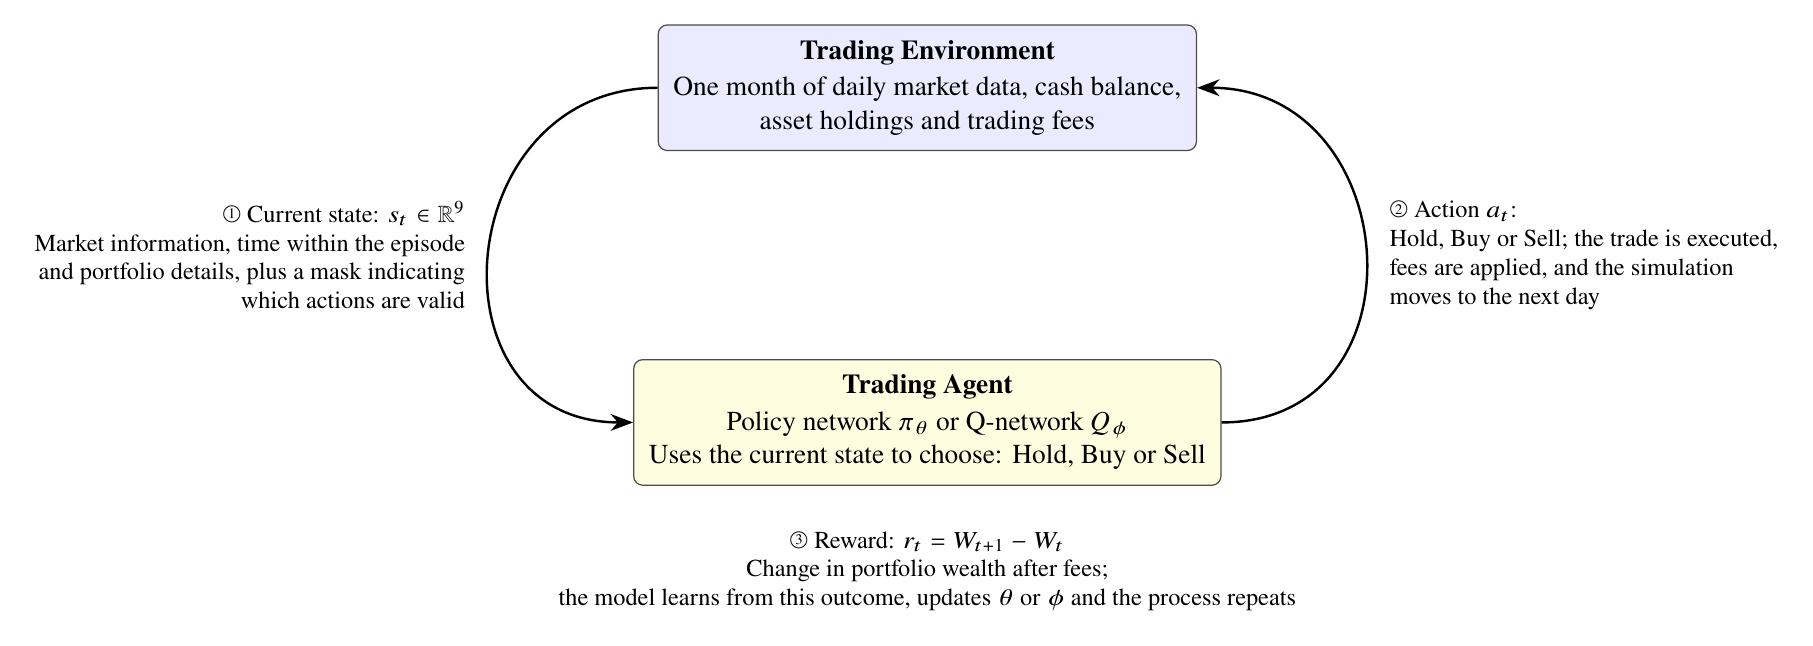
\includegraphics[width=0.9\textwidth]{media/media/image1_ch3.png}
  \caption[The agent--environment interaction loop for the trading MDP.]{The agent--environment interaction loop for the trading MDP. One cycle corresponds to one trading day.}
\end{figure}


To make the MDP formulation easier to understand, Table 3.2 compares the
main components of the trading task with those of a familiar
game-playing task, Flappy Bird, which was used initially to understand
Reinforcement Learning.

\addcontentsline{lot}{table}{\protect\numberline{3.2}{Mapping a popular game MDP to the portfolio trading MDP.}}
\textbf{Table 3.2: Mapping a popular game MDP to the portfolio trading
MDP.}

{\def\LTcaptype{none} % do not increment counter
\begin{longtable}[]{@{}
  >{\raggedright\arraybackslash}p{(\linewidth - 4\tabcolsep) * \real{0.2129}}
  >{\raggedright\arraybackslash}p{(\linewidth - 4\tabcolsep) * \real{0.3872}}
  >{\raggedright\arraybackslash}p{(\linewidth - 4\tabcolsep) * \real{0.3998}}@{}}
\toprule\noalign{}
\begin{minipage}[b]{\linewidth}\raggedright
\textbf{MDP component}
\end{minipage} & \begin{minipage}[b]{\linewidth}\raggedright
\textbf{Flappy Bird}
\end{minipage} & \begin{minipage}[b]{\linewidth}\raggedright
\textbf{Trading (this work)}
\end{minipage} \\
\midrule\noalign{}
\endhead
\bottomrule\noalign{}
\endlastfoot
State \emph{s\textsubscript{t}} & Bird\textquotesingle s position and
speed, together with the position of the next pipe & Market information
and the agent\textquotesingle s current portfolio position \\
\rowsep
Action \emph{a\textsubscript{t}} & Flap or do not flap & Hold, Buy, or
Sell \\
\rowsep
Reward \emph{r\textsubscript{t}} & Survival score based on how long the
bird remains in play & Change in portfolio wealth after trading fees \\
\rowsep
Episode \emph{τ} & One complete game session & One calendar month of
daily trading \\
\rowsep
Terminal rule & The game ends when the bird crashes or hits the ground &
The episode ends at the final trading day, with any remaining position
sold \\
\end{longtable}
}

This analogy also highlights a design principle used throughout the
project: as the Flappy Bird state contains the information relevant to
the next decision, the trading state includes the relevant information
available to the agent at each trading step, without being given future
information. Section 3.3 discusses the design of the trading state in
more detail.

\section{Episode Definition and Data Structure}

\subsection{Episode definition \texorpdfstring{\((\tau)\)}{()}}

Each episode \((\tau)\) represents one calendar month of daily closing
prices, from \(P_{0}\ to\ P_{T}\) \((P_{0},\ \ P_{1},\ldots,P_{T})\)
where \(T\) is typically between 18 and 23 trading days per month,
excluding public holidays when markets aren't open and weekends of
market inactivity \((T \approx 18 - 23)\). At the beginning of each
episode, the agent starts with cash and no asset holdings. It can then
trade throughout the month based on the available information. At the
end of the final trading day \(t\), any remaining position is
automatically sold. This ensures that no position is carried over from
one episode to the next.

\subsection{Independence of Trading Episodes}

For the purposes of the experiment, each monthly episode is treated as a
separate and independent trading period. This is similar to treating
each game session in Flappy Bird as a separate episode.

However, this is a simplification because market conditions in
consecutive months are not truly independent. For instance, events and
trends in one month do influence the market in the following month. The
resulting data are therefore not independent over time.

Modelling these temporal relationships in greater detail would require
time-series or partially observable approaches, which are outside the
scope of this project. The implications of this assumption are discussed
further in the conclusion\textbf{.}

\subsection{Choice of Episode Length}

Monthly episodes were selected to provide a balance between the length
of each trading period and the total number of training examples
available.

A single year of daily data provides approximately 12 monthly episodes
and around 250 daily trading decisions. Using eight years of data from
2018 to 2025 gives 96 monthly episodes and approximately 2,000 daily
transitions. These episodes are divided chronologically into 60 months
for training, 12 months for validation, and 24 months for the held-out
test period, as detailed in Chapter 4. The data are not shuffled, which
prevents information from later periods from being used during training
and helps avoid look-ahead leakage.

The same environment could also be adapted to shorter intervals, such
as minute-level data, without a fundamental change to its design, but
intraday trading is outside the scope of this study.

\subsection{Selection of the Historical Period}

The experiments use daily market data from 2018 to 2025 as a fixed
period. Earlier data, including data from 2016 and before, were not
included in the main experimental period because the study aims to
evaluate the learning algorithms under relatively recent and varied
market conditions. These selected periods contain a range of market
conditions, including relatively stable periods in 2018, the market
decline associated with the COVID-19 pandemic and its subsequent
recovery, the later period of increased inflation and interest rates,
and the war in Ukraine in 2022, which caused weaker market conditions.
As a result, the dataset is not limited to a single type of market
condition, providing a useful range for evaluating the behaviour of the
portfolios trading agents without extending the dataset into
substantially older market years.

Including older data, such as 2016 or earlier, would increase the
number of observations but could also introduce market conditions that
differ considerably from those in the selected period, such as older
microstructure and fee regimes. Earlier historical data are therefore
left to future work as an additional robustness test of how well the
trained agents generalise across market regimes.

It should also be noted that real financial markets are more complex
than any MDP and cannot be assumed to be fully observable. The MDP used
here is a simplified representation of the portfolio trading problem;
the information the agent cannot observe, and the consequences of this,
are discussed with the state representation in Section 3.3.

\section{State Representation Design}

In reinforcement learning, how information is presented to the agent
plays an important role in the quality of decisions it can learn. The
state representation must provide enough information for the agent to
understand the current situation and choose an appropriate action.

In this portfolio trading problem, this requires capturing information
about both the market and the agent\textquotesingle s own portfolio. The
agent needs to know how the asset has been moving, but it also needs to
know how much cash is available, whether it currently holds the asset,
whether that position is profitable, and how much time remains before
the trading period ends.

A state that leaves out important information can make it difficult for
the agent to learn effective strategies, even if the learning algorithm
is suitable for the task. This is because the agent can make decisions
only using the information provided. Therefore, the state representation
in this study was developed gradually by first examining simpler
representations and then adding information as needed to address
specific limitations of the previous representation.

The objective was not to create an unnecessarily complex state
representation with many variables, but to design a compact
representation containing all relevant information needed for
decision-making within the defined portfolio trading environment, while
avoiding features that simply duplicate information already available
from other variables

\subsection{Information Available to the Agent}

As discussed in Section 3.1, the state should see the whole by providing
the agent with information relevant to its decision, as the Flappy Bird
state does. In a trading environment, this information can be divided
into two halves: \textbf{the agent\textquotesingle s own portfolio} and
\textbf{the wider market}. These two areas behave very differently and
should therefore be considered separately when designing the state.

The first area is the agent\textquotesingle s own portfolio. This
includes information such as the amount of cash available, how much of
the asset it owns, what it paid to enter a trade position, and the time
remaining in the trading period. The agent controls this half; it is not
hidden or estimated, and it can be completely represented. Given the
sequence of the asset prices and the agent\textquotesingle s actions,
the portfolio can be updated directly using the trading environment's
rules.

The second area is the market. Here, complete information about the
market is impossible in principle and cannot be provided to the agent
because many factors affecting an asset's price are not directly
observable from the available price data. For example, the agent cannot
observe other market participants\textquotesingle{} decisions,
expectations, or intentions. Similarly, information such as news, market
sentiment, and macroeconomic events may influence prices without
appearing directly in the closing price at the end of the episode.

Adding more features calculated from past prices can give the agent
additional information about recent market behaviour, but it cannot
reveal everything happening in the market. The attainable goal is
therefore a state that is complete on the portfolio side and rich
enough on the market side: \textbf{the portfolio information can be
represented completely because the environment directly controls and
records it, whereas market information can only approximate the wider
market.} Whether the additional market features provide useful
information is ultimately an empirical question, which is considered
when evaluating the state representation later in the dissertation.

\subsection{Criteria for a Suitable Trading State}

It is tempting to design a state by asking which features look useful,
but this is a weak approach as it says nothing about whether the object
being trained is an MDP at all.

Before deciding on the final state representation, three conditions were
considered. These provide a basis for deciding whether the proposed
state contains the information required for the portfolio trading
problem.

\textbf{1. Reward measurability}

The reward should be calculable from information available to the agent
and the resulting transition. If the reward depends on information not
contained in the state or the transition, the agent is effectively being
evaluated using information it cannot observe.

The primary reward used in this study is the change in portfolio wealth,
\(r_{t} = W_{t + 1} - W_{t}\). The final state includes cash and asset
exposure as fractions of the initial capital, and these two features
combine to give the current wealth, so the reward can be calculated
from the observed transition \((s_{t},a_{t},s_{t + 1})\) with no hidden
portfolio variable. Section 3.5 defines the reward and shows this
derivation in full.

\textbf{2. Transition consistency}

The state should also contain enough information for the next state to
be determined from the current state, the selected action, the next
observed market price, and the trading environment rules.

This matters because the agent should not need to access hidden
historical variables to describe how its portfolio changes after an
action.

For example, the current portfolio exposure can be used to determine the
position's value, while the current unrealised profit/loss contains
information about the position\textquotesingle s entry price. Together
with the current price and the environment\textquotesingle s trading
rules, these quantities provide the information required to update the
portfolio after an action.

This keeps the state representation consistent with the defined trading
environment rather than requiring the environment to retrieve additional
portfolio history that is not represented in the state.

\textbf{3. Decision sufficiency}

The state should contain enough information for the agent to make a
decision based on the current trading situation without ambiguity. If
two different situations look identical to the agent but require
different actions, then the state is missing important information,
making the representation incomplete.

For example, consider the following two situations:

\begin{itemize}
\item
  the asset price has increased by 2\% today, and the agent does not
  hold the asset;
\item
  the asset price has increased by 2\% today, but the agent holds a
  position that is currently making a loss.
\end{itemize}

In both cases, the observed price movement is the same. However, the
most appropriate action may be different. In the first situation, the
agent may consider opening a position, whereas in the second, it may
consider reducing or closing its existing position to minimize its
losses.

The state representation must therefore include information about both
the market and the agent\textquotesingle s own portfolio.

\subsection{Development of the State Representation}

The state was developed in stages, starting from the smallest
representation that could describe a trading decision and adding
information only where the previous stage left the agent unable to
distinguish situations that require different actions. Table 3.4 at the
end of this section summarises the full progression.

The starting point was a price-only state,
\(s_{t}^{(0)} = \left\lbrack \Delta P_{t} \right\rbrack\), where
\(\Delta P_{t} = (P_{t} - P_{t - 1})/P_{t - 1}\) is the one-day return.
This is insufficient because the same market movement can occur in very
different trading situations. A positive daily return means one thing
when the agent holds nothing and may consider entering a position, and
another when it already holds a large position and may consider reducing
it. The agent cannot see its own portfolio.

Portfolio, position, and time information were therefore added in turn,
producing the following features:

\textbf{1. Normalised cash} \(\mathbf{(c}_{\mathbf{t}}\mathbf{)}\),
defined as \(c_{t} = C_{t}/C_{0}\), is the proportion of the initial
capital that remains available for future decisions. Using a normalised
value keeps the information consistent regardless of the starting
account size.

\textbf{2. Normalised exposure} \(\mathbf{(v}_{\mathbf{t}}\mathbf{)}\),
defined as \(v_{t} = h_{t}P_{t}/C_{0}\), is the current market value of
the open position relative to the initial capital. This replaces the raw
unit count \(h_{t}\) because the same number of units can represent a
small or large investment depending on the asset price. Together, the
two portfolio features recover the agent\textquotesingle s current
wealth as \(c_{t} + v_{t} = W_{t}/C_{0}\).

\textbf{3. Unrealised profit/loss}
\(\mathbf{(Pn}\mathbf{L}_{\mathbf{t}}\mathbf{)}\):

\[PnL_{t} = \frac{P_{t} - {\overline{P}}_{t}^{entry}}{{\overline{P}}_{t}^{entry}}\]

where \({\overline{P}}_{t}^{entry}\) is the average price at which the
current position was opened. This tells the agent whether its position
is in profit or loss --- two situations that look identical from the
market side but may call for different actions. Holding an asset after
a price increase may be profitable if it was bought at a lower price,
or losing money if the position was entered at a higher price before
the price declined.

\textbf{4. Episode clock} \(\mathbf{(\tau}_{\mathbf{t}}\mathbf{)}\),
defined as \(\tau_{t} = t/T\), where \(T\) is the total length of the
episode. A value close to 0 means the episode has just started, while a
value close to 1 means the forced close at the final trading day is
approaching. This matters because the same action can have different
consequences depending on when it is taken: buying early leaves the
position time to grow, whereas buying shortly before the episode ends
does not.

\subsection{Final State Representation}

Although the previous stages successfully introduced information about
the agent's portfolio and position, they provide limited understanding
of the broader market conditions. A trading decision should not depend
only on the most recent price change, as different market situations
exist, producing similar short-term movements.

For this reason, the agent also needs information that helps it
distinguish between market conditions: whether the asset is in a
short-term upward or downward trend, whether the market is stable or
highly volatile, and whether the current price is above or below its
recent average level. Additional market-related features are therefore
included to give the agent a more complete view of the trading
environment.

The final state representation is defined as:

\[\boxed{s_{t}^{(4)} = \left\lbrack \Delta P_{t},mom_{t},vol_{t},gap_{t},{rng_{t},\tau}_{t},c_{t},v_{t},PnL_{t} \right\rbrack \in \mathbb{R}^{9}}\]

The following variables were added:

\textbf{1. Momentum}

\[mom_{t} = \frac{P_{t} - P_{t - k}}{P_{t - k}}\]

where \(k = 5\) previous days (about one trading week). Momentum gives
the agent a longer view of the recent price direction, helping it
differentiate a temporary movement from a more consistent trend
developing over several timesteps.

\textbf{2. Volatility}

\[vol_{t} = \sigma\left( \Delta P_{t - k + 1},...,\Delta P_{t} \right)\]

where \(\sigma\) is the standard deviation of the last \(k = 5\) daily
returns. This helps the agent recognise differences in market
uncertainty: a 2\% price increase during a relatively stable period is
different from a 2\% increase during a period of large and frequent
price movements, which indicates a riskier situation.

\textbf{3. Price trend position}

\[gap_{t} = \frac{P_{t}}{MA_{m,t}(P)_{t}} - 1\]

where \({MA}_{m,t}(P) = \frac{1}{m}\sum_{i = 0}^{m - 1}P_{t - i}\) is
the simple moving average of the closing price over the previous
\((m = 20)\) days (about one trading month). A positive value means the
current price is above its recent average level and a negative value
means it is below, helping the agent identify potential trends or
deviations from normal price behaviour.

\textbf{4. Normalised Trading Range}

The normalised trading range is based on the Average True Range (ATR):

\[rng_{t} = \frac{ATR_{n,t}}{P_{t}}\]

The True Range at timestep \(t\) is
\(TR_{t} = \max\left( H_{t} - L_{t},\,\left| H_{t} - C_{t - 1} \right|,\,\left| L_{t} - C_{t - 1} \right| \right)\),
where \(H_{t}\) and \(L_{t}\) are the current high and low prices and
\(C_{t - 1}\) is the previous closing price. The ATR is the rolling
arithmetic mean of the last \((n = 14)\) True Range values (about two
trading weeks):

\[ATR_{n,t} = \frac{1}{n}\sum_{i = 0}^{n - 1}TR_{t - i}\]

The ATR therefore measures the size of recent price movement using the
asset's high, low, and closing prices, and dividing it by the current
price creates a normalised measure that can be compared across different
price levels.

The nine features and what each tells the agent are
summarised in Table 3.3.

\addcontentsline{lot}{table}{\protect\numberline{3.3}{Full State Definition}}
\textbf{Table 3.3: Full State Definition}

\emph{Table 3.3: The} \emph{nine-feature state representation
(s\textsubscript{t} ∈ ℝ\textsuperscript{9}) used in the main
experiments. C\textsubscript{0} denotes the initial cash,
h\textsubscript{t} the number of asset units held, and
W\textsubscript{t} = C\textsubscript{t} + h\textsubscript{t}
P\textsubscript{t} the portfolio wealth at time t. the mark-to-market
wealth. The feature timestep lengths are set to (k=5) for momentum and
volatility, (m=20) for the moving-average reference, and (n=14) for the
Average True Range.}

{\def\LTcaptype{none} % do not increment counter
\begin{longtable}[]{@{}
  >{\raggedright\arraybackslash}p{(\linewidth - 6\tabcolsep) * \real{0.0521}}
  >{\raggedright\arraybackslash}p{(\linewidth - 6\tabcolsep) * \real{0.1159}}
  >{\raggedright\arraybackslash}p{(\linewidth - 6\tabcolsep) * \real{0.2666}}
  >{\raggedright\arraybackslash}p{(\linewidth - 6\tabcolsep) * \real{0.5653}}@{}}
\toprule\noalign{}
\begin{minipage}[b]{\linewidth}\raggedright
\textbf{\#}
\end{minipage} & \begin{minipage}[b]{\linewidth}\raggedright
\textbf{Feature}
\end{minipage} & \begin{minipage}[b]{\linewidth}\raggedright
\textbf{Definition}
\end{minipage} & \begin{minipage}[b]{\linewidth}\raggedright
\textbf{What it tells the agent}
\end{minipage} \\
\midrule\noalign{}
\endhead
\bottomrule\noalign{}
\endlastfoot
\multicolumn{4}{@{}>{\raggedright\arraybackslash}p{(\linewidth - 6\tabcolsep) * \real{1.0000} + 6\tabcolsep}@{}}{%
\emph{\textbf{Market}}} \\
\rowsep
1 & \emph{ΔP\textsubscript{t}} & \emph{P\textsubscript{t}} -
\emph{P\textsubscript{t−1}}/ \emph{P\textsubscript{t−1}} & The most
recent price movement \\
\rowsep
2 & \emph{mom\textsubscript{t}} & \emph{P\textsubscript{t}} -
\emph{P\textsubscript{t−k}}/ \emph{P\textsubscript{t−k}} & whether that
recent price movement is part of a short-term trend \\
\rowsep
3 & \emph{vol\textsubscript{t}} &
\(\sigma\left( \Delta P_{t - k + 1},...,\Delta P_{t} \right)\) & how
much the asset price has been varying recently \\
\rowsep
4 & \emph{gap\textsubscript{t}} & \emph{P\textsubscript{t}} /
MA\emph{\textsubscript{m}}(P) − 1 & how far the current price is from
its recent average \\
\rowsep
5 & \emph{rng\textsubscript{t}} & ATR\emph{\textsubscript{n}}(P) /
\emph{P\textsubscript{t}} & The size of the recent price ranges, which
closing prices alone cannot show \\
\rowsep
\multicolumn{4}{@{}>{\raggedright\arraybackslash}p{(\linewidth - 6\tabcolsep) * \real{1.0000} + 6\tabcolsep}@{}}{%
\emph{\textbf{Portfolio}}} \\
\rowsep
6 & \emph{c\textsubscript{t}} & \emph{C\textsubscript{t}} /
\emph{C\textsubscript{0}} & how much of the initial cash remains
available as cash \\
\rowsep
7 & \emph{v\textsubscript{t}} & \emph{h\textsubscript{t}}
\emph{P\textsubscript{t}} / \emph{C\textsubscript{0}} & The current
value of the open position relative to the initial capital \\
\rowsep
\multicolumn{4}{@{}>{\raggedright\arraybackslash}p{(\linewidth - 6\tabcolsep) * \real{1.0000} + 6\tabcolsep}@{}}{%
\emph{\textbf{Position}}} \\
\rowsep
8 & \emph{PnL\textsubscript{t}} & (\emph{P\textsubscript{t}} −
\emph{P̄\textsubscript{tentry}}) / \emph{P̄\textsubscript{tentry}} &
whether the open positions are in profit or loss \\
\rowsep
\multicolumn{4}{@{}>{\raggedright\arraybackslash}p{(\linewidth - 6\tabcolsep) * \real{1.0000} + 6\tabcolsep}@{}}{%
\emph{\textbf{Time}}} \\
\rowsep
9 & \emph{τ\textsubscript{t}} & \emph{t} / \emph{T} ∈ {[}0, 1{]} & how
much time remains before the trading episode ends \\
\end{longtable}
}

\subsection{Feature Redundancy and Excluded Information}

The state was not designed by adding every potentially useful market
indicator. Features were included only where they provide information
that cannot already be recovered from the other variables in the state.

This is important because adding a feature that simply repeats existing
information increases the size of the input without providing the agent
with anything new.

The following features were excluded:

\textbf{1. Running portfolio return}

For example, the portfolio\textquotesingle s current return relative to
its starting capital\\
does not need to be included as a separate feature because it can
already be calculated from the normalised cash and asset exposure as
\(c_{t} + v_{t}\). Adding it would duplicate information already
available in the state.

\textbf{2. Raw position size}

The raw number of units held, \(h_{t}\), is also not included in the
final state. The financial value of the position is more directly
represented by:

\[v_{t} = \frac{h_{t}P_{t}}{C_{0}}\]

This provides information about the actual exposure rather than only the
number of units.

\textbf{3. Raw asset price}

The raw asset price is also not required as a separate feature. The
state instead uses returns and normalised values, which describe price
movements without depending on the standard price level.

The general principle is therefore to include features that provide
useful information while avoiding variables that can already be
reconstructed from information available elsewhere in the state.

\subsection{The Risk-Aware Extension: Drawdown State}

The main state representation contains the information needed for the
change in wealth reward. However, it does not describe the history of
the portfolio's losses: current wealth alone does not show how the
portfolio reached its current value. For example, two portfolios can
have exactly the same wealth at the current timestep but may have
followed very different paths:

\begin{itemize}
\item
  one portfolio may have increased steadily over time;
\item
  another may have suffered a large loss before recovering to the same
  level.
\end{itemize}

To address this, an additional feature representing portfolio drawdown
is introduced as a separate risk-aware extension:

\[dd_{t} = \frac{\max_{u \leq t}W_{u} - W_{t}}{\max_{u \leq t}W_{u}}\]

where \(dd_{t}\) represents the current decline in portfolio wealth from
the highest wealth level reached so far during the episode.

A value of zero means that the portfolio is currently at its highest
wealth level reached so far in the episode. A larger value indicates
that the portfolio has fallen further below its previous peak.

For this reason, drawdown is treated separately from the main state
representation. This makes it possible to evaluate whether explicitly
providing information about portfolio loss history affects the
agent\textquotesingle s behaviour and performance.

The resulting risk-aware state is therefore:

\[s_{t}^{risk} \in R^{10}\]

where:

\[s_{t}^{risk} = \left\lbrack s_{t},dd_{t} \right\rbrack\]

Since the original state \(s_{t}\) contains nine features, adding
drawdown produces a \textbf{ten-dimensional} risk-aware state.

\subsection{Feature Calculation and Information Timing}

The timing of feature calculation matters because the agent should
receive only the information available when making its trading decision.
Using future information would give the agent an unfair advantage and
could lead to overly optimistic results.

For this reason, the market features are calculated using information
available at or before timestep \((t)\). The current price and past
prices can be used to create the state, but the agent must not use
future prices when it decides its action \((a_{t})\).

The same principle applies to the features that use historical windows:
momentum uses the previous \((k = 5)\) timesteps, the moving average the
previous \((m = 20)\) prices, and the normalised trading range the
\((n = 14)\)-day ATR, as reported in Table 3.3.

Therefore, each state is based only on information that is available at
the time the decision is made. This prevents future market information
from entering the agent\textquotesingle s observation and helps avoid
\textbf{look-ahead bias}, where a model appears to perform well because
it has indirectly been given information that would not have been
available during actual trading.

\subsection{State Representation Limitations}

Although the final state representation gives the agent a wider range of
information, the trading environment is still a simplified
representation of a real financial market.

The agent does not have access to several types of information that can
influence real-world trading decisions, including:

\begin{itemize}
\item
  order flows;
\item
  market sentiment;
\item
  financial news;
\item
  macroeconomic conditions;
\item
  relationships between the asset and other financial assets.
\item
  The actions and intentions of large financial institutions.
\end{itemize}

These limitations mean that the state should not be interpreted as a
complete description of the real financial market. Because this relevant
information cannot be represented in the environment, it is better to
describe this as a \emph{\textbf{partially observable Markov decision
process (POMDP)}} rather than a fully observable one.

However, this dissertation does not aim to replicate every aspect of
real-world financial markets. The purpose is to compare and evaluate
reinforcement learning algorithms within a controlled trading
environment for an asset.

The proposed state representation therefore provides sufficient
information for the defined task and can be \textbf{considered complete
with respect to} \textbf{the information used by the defined trading
environment}, which includes recent market behaviour, the current
portfolio position, the performance of its current position, and the
amount of time remaining in the trading period, while acknowledging that
the model does not capture all factors present in real-world trading.

\subsection{Summary}

The final state was not selected because it contained a particular
number of variables, but because its components collectively describe
the market conditions, portfolio exposure, position performance, and
remaining trading episode available within the defined environment.
Table 3.4 summarises the design progression and the limitation each
stage resolved.

\addcontentsline{lot}{table}{\protect\numberline{3.4}{The staged development of the state representation. Each stage resolves the limitation named in the row above it.}}
\emph{Table 3.4: The staged development of the state representation.
Each stage resolves the limitation named in the row above it.
ΔP\textsubscript{t} is the one-step return, c\textsubscript{t} cash and
v\textsubscript{t} exposure as fractions of initial capital,
h\textsubscript{t} the units held, τ\textsubscript{t} the episode clock
and dd\textsubscript{t} the fall from peak wealth.}

{\def\LTcaptype{none} % do not increment counter
\begin{longtable}[]{@{}
  >{\raggedright\arraybackslash}p{(\linewidth - 4\tabcolsep) * \real{0.1007}}
  >{\raggedright\arraybackslash}p{(\linewidth - 4\tabcolsep) * \real{0.3148}}
  >{\raggedright\arraybackslash}p{(\linewidth - 4\tabcolsep) * \real{0.5665}}@{}}
\toprule\noalign{}
\begin{minipage}[b]{\linewidth}\raggedright
\textbf{Stage}
\end{minipage} & \begin{minipage}[b]{\linewidth}\raggedright
\textbf{State}
\end{minipage} & \begin{minipage}[b]{\linewidth}\raggedright
\textbf{Limitation addressed by the next stage}
\end{minipage} \\
\midrule\noalign{}
\endhead
\bottomrule\noalign{}
\endlastfoot
\emph{S\textsubscript{0}} & {[}\emph{ΔP\textsubscript{t}}{]} & The agent
can observe recent price movement but has no information about its own
portfolio. It cannot tell whether it already holds the asset, or whether
it has enough cash to open a position. \\
\rowsep
\emph{S\textsubscript{1}} & {[}\emph{ΔP\textsubscript{t}},
\emph{c\textsubscript{t}}, \emph{h\textsubscript{t}}{]} & The agent now
knows its available cash and the number of units it holds but not what
they are worth. For example, ten units could represent a small or large
investment depending on the asset price. \\
\rowsep
\emph{S\textsubscript{2}} & {[}\emph{ΔP\textsubscript{t}},
\emph{c\textsubscript{t}}, \emph{v\textsubscript{t}},
\emph{PnL\textsubscript{t}}{]} & The agent can now determine the value
of its position and tell whether its in profit or loss, but it does not
know where it stands in the month. A position opened at the beginning of
the month can therefore appear identical to one made immediately before
the required closing of the position at the end of the month. \\
\rowsep
\emph{S\textsubscript{3}} & {[}\emph{ΔP\textsubscript{t}},
\emph{c\textsubscript{t}}, \emph{v\textsubscript{t}},
\emph{PnL\textsubscript{t}}, \emph{τ\textsubscript{t}}{]} & The
agent\textquotesingle s own circumstances are now fully represented, but
its view of the market is still limited to the most recent price return.
It cannot tell a stable trend from a reversal, or between relatively
stable and highly volatile conditions. \\
\rowsep
\emph{S\textsubscript{4}} & adds momentum, volatility, distance from
trend, and daily range (Table 3.3) & The state provides a broader
representation of the market while retaining the portfolios information.
It is treated as the main state used in the experiments. \\
\rowsep
\emph{S\textsubscript{risk}} & adds \emph{dd\textsubscript{t}} & Adds
information about the portfolio\textquotesingle s previous losses from
its highest wealth level. Required when the experiment considers risk
history \\
\end{longtable}
}

The separate tenth feature, drawdown, is used only for the risk-aware
experiments described in Section 3.3.6.

The main state representation provides the basis for defining the
available actions and applying the reinforcement learning algorithms
described in the following sections.

\section{Action Space Design}

\subsection{Overview}

The action space defines the choices available to the trading agent at
each timestep. Its design matters because it determines how the agent
interacts with the market and what its learned policy means.

A poorly designed action space can introduce unnecessary complexity or
create unrealistic trading behaviour. For example, allowing the agent to
choose any number of shares to buy or sell adds learning challenges: the
agent must simultaneously learn when to trade\textbf{,} which direction
to take\textbf{,} and how much to trade. This can make it difficult to
determine whether poor performance results from an ineffective trading
strategy or from difficulty learning appropriate position sizes.

To keep the focus on the trading decisions made by the reinforcement
learning algorithms, this study uses \textbf{a simplified discrete
action space}. The agent decides on the action (trading direction),
while the environment determines the amount traded.

This separates the trading problem into two decisions:

\begin{enumerate}
\def\labelenumi{\arabic{enumi}.}
\item
  \textbf{When and in which direction to trade} --- this is the trading
  policy being learned by the reinforcement learning algorithm.
\item
  \textbf{How much capital to trade} --- this is fixed by the
  environment and treated as an experimental setting.
\end{enumerate}

This approach keeps the action space simple and makes it easier to
compare the learning algorithms on the same portfolio trading task. It
also means that differences in performance can be interpreted mainly in
terms of the agents\textquotesingle{} ability to learn trading
decisions, rather than their ability to learn position sizing.

\subsection{Trading Actions and Trade Size}

The action space is defined as \(A = \left\{ 0,1,2 \right\}\), where
action 0 \textbf{holds} the current position, action 1 \textbf{buys} a
fixed amount, and action 2 \textbf{sells} a fixed amount. At each
timestep, the agent selects one of these three actions using the
information available in the current state.

The \textbf{hold} action leaves the portfolio unchanged. No transaction
takes place: the available cash and the number of units held remain the
same, and no transaction fee is charged. This allows the agent to remain
in its current position when it does not consider buying or selling to
be appropriate.

The \textbf{buy} and \textbf{sell} actions change the
agent\textquotesingle s exposure to the asset by a fixed monetary
amount:

\[\Delta = f\,C_{0}\]

where \(C_{0}\) is the initial capital and \(f\) is the fraction of that
capital allocated to one transaction. A fixed monetary amount is used
rather than a fixed number of shares because the cost of one share
depends heavily on the price level: buying one share of an asset priced
at \pounds 10 is a small investment, while buying one share priced at
\pounds 1,000 is a large one, even though both would be described as
buying one share. Fixing the monetary size keeps every trade at the same
proportion of the initial capital throughout the dataset, regardless of
the asset price.

The fraction \(f\) is treated as an experimental setting rather than a
fixed design constant. It is selected using the validation data before
the final experiments, as reported in Section 5.3.

The number of units bought or sold at price \(P_{t}\) is:

\[\Delta h_{t} = \pm\frac{\Delta}{P_{t}}\]

with the positive sign for a buy and the negative sign for a sell, and
with fractional ownership allowed, similar to a real-world portfolio. A
sell is valid only when the agent holds enough units for the transaction.
Because the trade size is fixed, the agent can build or reduce its
position gradually over several decisions while still operating within a
simple three-action framework.

\subsection{Action Constraints}

Although the agent has three possible actions, some actions may not be
possible at a particular timestep because of the current portfolio
position.

For example:

\begin{itemize}
\item
  the agent cannot buy if it does not have enough available cash;
\item
  the agent cannot sell if it does not hold enough of the asset to
  withdraw.
\end{itemize}

To handle these situations, the environment uses a \textbf{legal action
mask}. The mask does not provide any additional market information to
the agent. It simply indicates which actions can be carried out given
the current portfolio status.

The mask is represented as
\(M_{t} = \left\lbrack m_{\text{hold}},m_{\text{buy}},m_{\text{sell}} \right\rbrack \in \left\{ 0,1 \right\}^{3}\),
where \(M_{t}(a) = 1\) indicates that action \(a\) is available and
\(M_{t}(a) = 0\) indicates that it is not.

The availability of each action is determined from the portfolio state:

\begin{itemize}
\item
  available cash determines whether a \textbf{buy} action can be carried
  out;
\item
  the current asset holding determines whether a \textbf{sell} action
  can be carried out;
\item
  \textbf{hold} remains available throughout the episode.
\end{itemize}

Because the mask is derived directly from information already in the
portfolio state, it is not treated as an additional feature of the state
representation. Instead, it acts as a constraint on the agent,
preventing it from selecting actions the environment cannot execute.

\subsection{Transaction Costs}

A transaction fee of \(c = 0.05\%\) is charged whenever the agent
carries out a buy or sell action, so a transaction of value \(\Delta\)
incurs a fee of \(\Delta c\). The same fee calculation is applied to
both purchases and sales.

Including transaction costs matters because it prevents the agent from
overly buying and selling repeatedly. Without these fees, the agent
could benefit from making many trades even when price movements are very
small, making frequent trading appear more profitable than it would be
in practice.

The inclusion of fees therefore introduces a basic cost of trading into
the environment and provides a more realistic basis for evaluating
learned trading strategies.

\subsection{Relationship Between the State and Actions}

The action space was designed to match the state representation of
Section 3.3. Deciding whether to buy or sell depends on the
agent\textquotesingle s current exposure, its available cash, whether an
existing position is in profit or loss, the time remaining in the
episode, and the current market conditions --- exactly the information
the state provides. The agent decides whether to hold, buy, or sell,
while the environment determines the amount traded and prevents invalid
actions from being carried out.

\section{Reward Function Design}

\subsection{Purpose of the Reward Function}

The reward function tells the reinforcement learning algorithm how well
it performed after taking an action and guides the agent toward more
desirable actions. Unlike supervised learning, where the model is given
the correct answer, the agent learns by taking actions and receiving
feedback on the results of those actions.

In a trading environment, the reward function needs to accurately
reflect the actual objective of the investment strategy. If it is poorly
designed, the agent may learn behaviours that are not desirable, such as
trading too frequently, taking unnecessary risks, or performing well
during training but poorly under realistic conditions.

The main goal of this dissertation is to investigate whether
reinforcement learning algorithms can learn profitable trading
strategies for the selected asset while accounting for transaction
costs. For this reason, the primary reward is based on the
\textbf{change in portfolio wealth} from one timestep (trading day) to
the next.

\subsection{Wealth-Based Reward}

The main reward used in this study is based on the change in the
portfolio\textquotesingle s total value:

\[r_{t} = W_{t + 1} - W_{t}\]

where portfolio wealth at timestep \(t\) is given by:

\[W_{t} = C_{t} + h_{t}P_{t}\]

Here:

\begin{itemize}
\item
  \(C_{t}\) represents the cash available in the portfolio;
\item
  \(h_{t}\) represents the number of asset units held;
\item
  \(P_{t}\) represents the current asset price.
\end{itemize}

The reward therefore measures how much the portfolio\textquotesingle s
total value changes from one timestep (trading day) to the next after
the agent\textquotesingle s action.

A \textbf{positive reward} means the portfolio increased in value, while
a \textbf{negative reward} means it decreased. This gives the agent a
direct measure of the financial outcome of its decisions.

\subsection{Including Transaction Costs in the Reward}

Transaction fees are included when calculating the reward so that the
result reflects the actual cost of carrying out a trade.

When a buy or sell action is taken at timestep \(t\), the portfolio
value is updated after the transaction fee is deducted:

\[W_{t + 1} = C_{t + 1} + h_{t + 1}P_{t + 1} - Fees\]

The reward is then calculated from the resulting change in portfolio
wealth. This means that the agent is rewarded or penalised based on the
value of the portfolio \textbf{after trading costs have been taken into
account}.

\subsection{Wealth Change As the Primary Reward}

The change in portfolio wealth was chosen as the main reward for several
reasons.

First, it directly reflects the main objective of the trading strategy:
\textbf{increasing the value of the portfolio}. This also makes the
reward closely related to the metric used to evaluate investment
performance in the real world.

Second, it satisfies the requirements of the MDP defined in Section 3.2
because the reward can be obtained from portfolio information in the
state representation.

The current portfolio wealth can be recovered from the cash and exposure
features in the state representation:

\[c_{t} + v_{t} = \frac{W_{t}}{C_{0}}\]

Therefore, the change in wealth can be written as:

\[W_{t} = C_{0}\left\lbrack \left( c_{t} + v_{t} \right) \right\rbrack\]

\[r_{t} = C_{0}\left\lbrack \left( c_{t + 1} + v_{t + 1} \right) - \left( c_{t} + v_{t} \right) \right\rbrack\]

This shows that the reward depends only on the observed transition
\(\left( s_{t},a_{t},s_{t + 1} \right)\), without requiring additional
information unavailable to the agent.

\subsection{Risk-Aware Reward Extension}

Although the main objective is to increase portfolio wealth, focusing
only on returns may encourage the agent to take more risk than desired.
For example, a strategy may achieve a high final return but experience
large losses along the way, which is not a desirable trading behaviour.

Therefore, a risk-adjusted reward that accounts for changes in portfolio
drawdown is considered as an additional experimental condition:

\[r_{t}^{\mathrm{risk}} = \Delta W_{t} - \lambda\, C_{0}\, \Delta dd_{t}\]

where:

\begin{itemize}
\item
  \(\Delta W_{t}\) is the change in portfolio wealth;
\item
  \(\Delta dd_{t}\) is the increase in portfolio drawdown at step \(t\)
  (and is zero when drawdown does not rise);
\item
  \(C_{0}\) is the initial capital;
\item
  \(\lambda\) controls the penalty applied to increases in drawdown.
\end{itemize}

Drawdown measures how far the current portfolio wealth has fallen from
the highest level reached so far:

\[dd_{t} = \frac{\max_{u \leq t}W_{u} - W_{t}}{\max_{u \leq t}W_{u}}\]

where \(W_{t}\) is the portfolio wealth at time \(t\), and \(W_{u}\) is the
wealth at any earlier time \(u\) up to \(t\).
\(\max_{u \leq t}W_{u}\) is therefore the highest wealth reached so far
in the episode.

\(\Delta dd_{t}\) is therefore the increase in drawdown from one trading
day to the next. Multiplying it by the initial capital \(C_{0}\) keeps
the reward in dollars, so a penalty of \(\lambda = 0\) lets the
wealth-change reward remain the same, while a larger \(\lambda\)
discourages actions that worsen the drawdown.

However, this reward requires access to the
portfolio\textquotesingle s previous performance because the previous
highest wealth reached up to time \(t\) must be known in order to
calculate drawdown.

For this reason, the risk-aware reward is used only with the
\textbf{risk-aware state extension} described in Section 3.3.6. This
ensures that the information needed to calculate the reward is available
to the agent.

The wealth-change reward remains the main reward used in the baseline
experiments. The risk-aware version is treated separately so that the
effect of explicitly including information about portfolio loss history
can be examined.

\subsection{Limitations of the Reward Function}

Although the wealth-change reward provides a clear and direct measure of
trading performance, it does not capture every aspect of a desirable
trading strategy.

For Example, it does not directly penalise:

\begin{itemize}
\item
  large falls in portfolio value;
\item
  unstable performance in returns;
\item
  high levels of volatility.
\end{itemize}

A strategy could therefore achieve a strong overall return while
experiencing substantial losses during the trading period. The
limitations are addressed by the risk-aware reward in Section 3.5.5 by
adding a penalty when drawdown increases.

However, adding more objectives changes the learning problem and what
the agent is being trained to optimise. This can make comparisons
between algorithms less straightforward because improvements may result
from the different reward definition rather than from the learning
algorithm itself.

Therefore, the \textbf{wealth-change reward is used as the common
baseline}, while the risk-aware reward is considered separately as an
additional experiment.

\section{Objective Function}

The objective function describes what the reinforcement learning
algorithms are trying to achieve during training. In this study, the aim
is to learn a trading policy that produces the highest possible expected
return over each trading episode.

The reward function introduced in Section 3.5 measures the result of an
individual decision, while the objective function extends this idea by
combining the rewards received throughout the episode.

\subsection{Episode Return}

An episode/trajectory can be represented by the sequence:

\[\tau = \left( s_{0},a_{0},r_{0},s_{1},a_{1},r_{1},\ldots,s_{T} \right)\]

where \(s_{t}\) is the state observed at timestep \(t\),

\(a_{t}\)is the action selected by the agent, and

\(r_{t}\) is the reward resulting from that action.

The episode contains \(T\) trading decisions and ends when it reaches
the final market observation. Any position that remains open at this
point is then closed according to the rules of the trading environment.

The total discounted return from the beginning of the episode is:

\[G_{0} = \sum_{t = 0}^{T - 1}\gamma^{t}r_{t},\]

Where \(\gamma \in (0,1\rbrack\) is the discount factor.

The same calculation can be made from any point within the episode. The
return from timestep \(t\), commonly referred to as the
\textbf{reward-to-go}, is:

\[G_{t} = \sum_{t' = t}^{T - 1}\gamma^{t' - t}r_{t'}.\]

This represents the rewards expected from the current timestep onwards.
It is particularly relevant to the REINFORCE implementation because it
associates an action with the rewards that follow it, rather than
assigning the episode\textquotesingle s total return to every action
taken in that episode.

A discount factor of \(\gamma = 0.99\) is used throughout the
experiments. The trading episodes contain approximately 18--23 daily
observations, so this value results in relatively mild discounting over
the length of an episode: \({0.99}^{20} \approx 0.82\), so a reward
received near the end of the monthly episode still contributes around
82\% of its original value to the discounted return.

Using \(\gamma = 0.99\), therefore, maintains the standard
reinforcement-learning formulation for discounted returns while still
ensuring the objective is maximising end-of-month wealth.

\subsection{Expected Return}

The outcome of a single trading episode is not enough to judge the
quality of a policy because each episode can reflect different market
conditions experienced during that month. For instance, a policy that
performs well in one month may not perform equally well in another.
Therefore, the objective is defined using the expected returns the
policy earns across different trading episodes.

The policy is represented by

\[\pi_{\theta}\left( a|s \right),\]

where \(\theta\) represents the trainable parameters of the policy
network. For a given state, the policy assigns probabilities to the
available actions, allowing the agent to choose between Buy, Hold, and
Sell.

\[\pi_{\theta}\left( a_{t} \mid s_{t} \right) = \begin{bmatrix}
P\left( a_{t} = \text{Hold} \mid s_{t} \right) \\
P\left( a_{t} = \text{Buy} \mid s_{t} \right) \\
P\left( a_{t} = \text{Sell} \mid s_{t} \right)
\end{bmatrix}\]

The expected return is defined as:

\[J(\theta) = \mathbb{E}_{\tau \sim p_{\theta}(\tau)}\left\lbrack G_{0}(\tau) \right\rbrack\]

The learning objective is therefore:

\[\theta^{*} = \arg{\max_{\theta}{J(\theta)}}.\]

In simple terms, the aim is not for the agent to find a policy that
performs well in only one trading period. Instead, the agent should
learn policy parameters that produce good, expected performance across
the different monthly market episodes used during training.

The policy parameters affect the objective only through the actions the
agent selects: changing \(\theta\) changes the probabilities of choosing
Buy, Hold, or Sell in each state, and these decisions affect the
portfolio and, in turn, the rewards collected over the episode.

\subsection{Objective and the Trading Environment}

The formulation above also separates the trading
environment\textquotesingle s role from the learning
algorithm\textquotesingle s. The environment determines the market data,
the current portfolio state, the transaction costs, which actions are
currently valid, the resulting portfolio wealth, the reward, and whether
the episode has ended. The learning algorithm determines only how the
agent updates its policy or value function using that experience.

This separation is important for comparing the different learning
approaches in this dissertation. \textbf{REINFORCE, DQN, and PPO} use
the same state representation, action space and masking, market data,
and reward function, so differences in their results stem from how they
learn rather than from the conditions they operate under.

\section{REINFORCE: Monte-Carlo Policy Gradient}

REINFORCE is the first policy-gradient method used in this study. Unlike
value-based methods, which estimate how useful different actions are in
a given state, \textbf{REINFORCE directly learns a policy} that gives
probabilities to the available actions.

It provides a useful baseline because its main idea is straightforward.
The agent selects actions according to its current policy, observes the
resulting rewards, and then adjusts the policy so actions can lead to
better returns in the future.

\subsection{Policy Representation}

The policy is represented by a neural network with trainable parameters
\(\theta\). Given the current state \(s_{t}\), the network produces one
output, or logit, for each of the three possible actions
\(\left\{ \text{Buy},\ \text{Hold},\ \text{Sell} \right\}\).
Actions that are not permitted at the current timestep using the action
mask described in Section 3.4 are removed. The remaining logits are then
passed through a SoftMax function to produce the policy probabilities
\(\pi_{\theta}\left( a_{t}|s_{t} \right)\).

During training, the agent samples an action from this probability
distribution. This lets it try different actions and explore alternative
trading decisions rather than always choosing the action with the
highest probability.

During evaluation, the agent selects the valid action with the highest
probability without exploring.

The policy network used in this study has \textbf{two hidden layers,
each with 128 units}, and uses the hyperbolic tangent \(\tanh\) as the
activation function. The final layer produces one output for each of the
three available actions.

\subsection{Deriving the Policy-Gradient Objective}

The objective introduced in Section 3.6 is an expected return over
trading episodes:

\[J(\theta) = \mathbb{E}_{\tau \sim p_{\theta}(\tau)}\left\lbrack G_{0}(\tau) \right\rbrack.\]

To improve the policy, the learning algorithm needs to determine how a
small change to the policy parameters \((\theta)\) affects this expected
return. This requires calculating the gradient:

\[\nabla_{\theta}J(\theta).\]

The difficulty is that the probability of a complete trading episode
\(p_{\theta}(\tau)\) depends on the initial state, the actions selected
by the policy, and the resulting environment transitions
\(\left( s_{0},a_{0},r_{1},s_{1},a_{1},r_{2},...,s_{T} \right)\). It can
be written as:

\[p_{\theta}(\tau) = \rho\left( s_{0} \right)\prod_{t = 0}^{T - 1}\pi_{\theta}\left( a_{t}|s_{t} \right)P\left( s_{t + 1}|s_{t},a_{t} \right),\]

where \(\rho\left( s_{0} \right)\) represents the probability
distribution of initial states and

\(P\left( s_{t + 1}|s_{t},a_{t} \right),\) represents the environment's
transition to the next state \(s_{t + 1}\) given the current state and
action \({(s}_{t},a_{t})\).

The important point is that the policy parameters \((\theta)\) affect
the action probabilities\(\ \pi_{\theta}\left( a_{t}|s_{t} \right)\) but
not the market transition process. REINFORCE therefore does not need to
model this market transition explicitly, just the action probabilities.

So, we use the likelihood-ratio identity, which provides a way of
expressing the gradient \(\nabla_{\theta}J(\theta)\) using the
probability of the sampled episodes \(p_{\theta}(\tau)\):

\[\nabla_{\theta}p_{\theta}(\tau) = p_{\theta}(\tau)\nabla_{\theta}{\log p}_{\theta}(\tau).\]

The policy gradient can then be expressed as:

\[\nabla_{\theta}J(\theta) = \mathbb{E}_{\tau\sim p_{\theta}}\left\lbrack \nabla_{\theta}{\log p}_{\theta}(\tau){\ G}_{0}(\tau) \right\rbrack.\]

Since only the policy terms depend on \((\theta)\), this simplifies to

\[\nabla_{\theta}J(\theta) = \mathbb{E}_{\tau{\sim p}_{\theta}}\left\lbrack \sum_{t = 0}^{T - 1}\nabla_{\theta}{\log\pi}_{\theta}\left( a_{t}|s_{t} \right)G(\tau) \right\rbrack.\]

This is the basic policy-gradient expression REINFORCE uses in this
study.

In simple terms, the equation adjusts the probability of an action based
on the outcome that follows it. Actions resulting in higher returns are
encouraged by increasing their probability, while actions associated
with lower returns are made less likely.

\subsection{Reward-to-Go}

Using the complete episode return \(G(\tau)\) for every action is
inefficient because an action taken at time \(t\) cannot influence
rewards already received before that time. REINFORCE therefore weights
each action by the reward-to-go \(G_{t}\) defined in Section 3.6, so
only rewards from time \(t\) onwards are used when evaluating the
outcome associated with that decision.

The policy gradient can therefore be written as:

\[\nabla_{\theta}J(\theta) = \mathbb{E}\left\lbrack \sum_{t = 0}^{T - 1}\nabla_{\theta}{\log\pi}_{\theta}\left( a_{t}|s_{t} \right)G_{t} \right\rbrack.\]

where \(\nabla_{\theta}{\log\pi}_{\theta}\left( a_{t}|s_{t} \right)\)
is the direction in which the policy\textquotesingle s action
probability changes, and \(G_{t}\) is the return obtained after taking
action \(a_{t}\). This links each decision directly to the rewards that
followed it.

\subsection{Monte-Carlo Estimation}

The expectation \(\mathbb{E}\) in the policy-gradient equation cannot
normally be calculated because the full distribution of possible market
trajectories is unknown. REINFORCE therefore uses a Monte Carlo
approach: the agent interacts with the trading environment and uses the
resulting episodes to estimate the gradient.

For \(N\) sampled episodes, the gradient can be approximated as:

\[\nabla_{\theta}J(\theta) \approx \frac{1}{N}\sum_{n = 1}^{N}{\sum_{t = 0}^{T_{n} - 1}\nabla_{\theta}}{\log\pi}_{\theta}\left( a_{t}^{(n)}|s_{t}^{(n)} \right)G_{t}^{(n)}.\]

The superscript \(n\) represents the number of the sampled episode.

The gradient is therefore estimated from the average experience
collected from the sampled episodes.

This is why REINFORCE is described as a \textbf{Monte-Carlo
policy-gradient method}: The method does not require the agent to know
in advance how the market will move or to build a separate model of
future price changes. Instead, it learns how to estimate the expected
policy gradient from complete sampled episodes produced by its
interaction with the environment.

\subsection{Loss Function Used for Training}

Most neural-network frameworks are designed to minimise a loss function,
while reinforcement learning is to maximise expected rewards
\(J(\theta)\). The policy-gradient objective can therefore be written as
a loss by introducing a negative sign:

\[L(\theta) = - \frac{1}{N}\sum_{n = 1}^{N}{\sum_{t = 0}^{T_{n} - 1}{\log\pi}_{\theta}}\left( a_{t}^{(n)}|s_{t}^{(n)} \right)G_{t}^{(n)}.\]

The negative sign changes the original maximisation problem into a
minimisation problem that can be handled by the PyTorch optimiser.

The logarithm appears as a direct result of the likelihood-ratio
derivation above; it is not an additional trading assumption.

The implementation uses the \textbf{Adam optimiser}~\cite{kingma2015adam}
with a learning rate of \(10^{- 3}\).

During implementation, the sampled returns may also be normalised before
being used in the update. This helps control the gradient magnitude
across different training batches and can improve numerical stability.

\subsection{Strengths and Limitations}

REINFORCE is a suitable baseline for this project because its
formulation is relatively straightforward: it directly learns the
policy and does not require a separate model of the market, so
performance differences against more advanced algorithms are easier to
interpret.

Its main limitation is that \textbf{its gradient estimates can have high
variance} because they depend completely on episode returns, and
different episodes can produce very different outcomes even in similar
trading situations. This can make learning less stable, particularly
when training data is limited. Reward-to-go and standardised returns
reduce some of this variation, but they do not remove the
algorithm\textquotesingle s underlying high-variance nature.

For this reason, this provides motivation for comparing REINFORCE with
the other methods, \textbf{DQN and PPO,} to see whether they can achieve
a more stable or effective learning in the same trading environment.

\section{Deep Q-Learning}

Deep Q-learning provides a \textbf{value-based alternative} to
REINFORCE. Rather than directly learning the probability of selecting
each action, it estimates the value of each possible action in the
current state. This comparison is useful because both methods address
the same portfolio trading problem but learn in different ways.

\subsection{Action-Value Function}

The action-value function, commonly referred to as the
\textbf{Q-function}, is defined as \(Q^{\pi}(s,a)\):

\[Q^{\pi}(s,a) = \mathbb{E}_{\pi}\left\lbrack \sum_{k = 0}^{\infty}\gamma^{k}r_{t + k} \right\rbrack.\]

This represents the expected future return from taking action \(a\) in
state \(s\) and then continuing to follow policy \(\pi\).

The optimal action-value function is written as
\(Q^{*}\left( s_{t},a_{t} \right)\). It represents the highest expected
return that can be achieved from a given state when the best available
actions are selected

For the optimal action-value function, the Bellman optimality equation~\cite{bellman1957}
is:

\[Q^{*}\left( s_{t},a_{t} \right) = \mathbb{E}\left\lbrack r_{t} + \gamma\max_{a'}{Q^{*}\left( s_{t + 1},a' \right)} \right\rbrack.\]

In simple terms, the value of an action depends on two things:

\begin{enumerate}
\def\labelenumi{\arabic{enumi}.}
\item
  the reward received immediately after taking the action; and
\item
  the value of the opportunities available afterwards.
\end{enumerate}

This makes the Q-function a useful representation for the portfolio
trading problem because the agent has a small action space.

In practice, the optimal Q-function is approximated by a neural network.
Once the values of the available actions have been estimated, the agent
selects the action with the highest Q-value:

\[a_{t}^{*} = \arg{\max_{a \in \mathcal{A}_{\text{legal}}\left( s_{t} \right)}{Q^{*}\left( s_{t},a \right)}}.\]

Only legal actions are considered when making this choice. This is
important in the trading environment because, for example, the agent
cannot buy when it does not have enough cash or sell when it does not
hold enough of the asset.

\subsection{From Q-Learning to Deep Q-Learning}

Traditional tabular Q-learning stores a separate value for every
state-action pair in a table. This approach is not suitable for the
present portfolio trading problem here because the state contains
continuous variables and several different market and portfolio
features.

For example, volatility and portfolio exposure can take many different
values. Converting all nine state features into discrete categories
would first require discretising the continuous variables and then
creating a very large state space that would also lose information by
grouping different values together.

Deep Q-learning avoids this problem by replacing the table with a neural
network \(Q_{\phi}(s,a)\), where \(\phi\) represents the trainable
parameters of the network.

The network takes the nine-dimensional state
\(s_{t} \in \mathbb{R}^{9}\) as input and estimates the Q-value for
each available action. These values are then used to select the most
valuable valid action, as in Section 3.8.1.

The DQN used in the experiments has \textbf{two hidden layers with 128
units each} and uses ReLU activation functions.

\subsection{Experience Replay}

Successive decisions within a trading episode are naturally related
because they come from consecutive trading days. If the network were
trained directly on these transitions in their original order, it could
produce highly correlated consecutive updates.

DQN addresses this issue using an \textbf{experience replay buffer}~\cite{lin1992, mnih2015}.
Each interaction with the environment is stored as a transition in a
memory buffer:

\[\left( s_{t},a_{t},r_{t},s_{t + 1},M_{t + 1},d_{t} \right),\]

where:

\begin{itemize}
\item
  \(s_{t}\) is the current state;
\item
  \(a_{t}\) is the action selected by the agent;
\item
  \(r_{t}\)is the reward received;
\item
  \(s_{t + 1}\)is the next state;
\item
  \(M_{t + 1}\)is the action mask for the next state;
\item
  \(d_{t}\)indicates whether the episode has ended.
\end{itemize}

During training, the agent samples random minibatches of previously
stored transitions from the replay buffer so the network does not rely
only on the most recent transition.

The replay buffer has a capacity of \textbf{50,000 transitions}, with
\textbf{64 transitions sampled per minibatch}.

This lets the network learn from reusable experiences collected at
different points during training and reduces the dependence between
consecutive training samples.

\subsection{Target Network}

Using the same network to calculate both the current Q-values and the
target values can make training unstable. This is because the network
parameters change during training, which also causes the target used for
learning to change.

To reduce this problem, DQN uses a second network known as the
\textbf{target network}~\cite{mnih2015}, \(Q_{\phi^{-}}(s,a)\).

The target network is kept separate from the main, or online, Q-network.
Rather than updating it after every gradient optimisation step, its
parameters are periodically copied from the main Q-network.

Keeping a fixed number of updates for the target provides a more stable
reference for calculating the temporal-difference target and reduces how
rapidly the learning target changes while the main network is being
updated.

In this implementation, the target network is synchronised with the
online network every \textbf{500 training steps}.

\subsection{Temporal-Difference Learning}

Unlike REINFORCE, which waits until the end of an episode to calculate
the return, DQN updates its estimates using a one-step
temporal-difference target.

For a transition, \(\left( s_{t},a_{t},r_{t},s_{t + 1} \right),\) the
target Q-value \(y_{t}\) is calculated from the immediate reward and the
highest estimated value of the best valid action in the next state:

\[y_{t} = r_{t} + \gamma\max_{a' \in \mathcal{A}_{\text{legal}}\left( s_{t + 1} \right)}{Q_{\phi^{-}}\left( s_{t + 1},a' \right)}.\]

Action masking is applied here because the agent should not assign value
to actions it cannot take in the next state.

When the episode ends, there are no future trading decisions or rewards
to consider. The target must therefore account for this condition:

\[y_{t} = r_{t} + \gamma\left( 1 - d_{t} \right)\max_{a' \in \mathcal{A}_{\text{legal}}\left( s_{t + 1} \right)}{Q_{\phi^{-}}\left( s_{t + 1},a' \right)}.\]

Where \(d_{t}\) indicates whether the episode has ended.

When \(d_{t} = 1\), the second term \(\left( 1 - d_{t} \right)\) becomes
zero, leaving \(y_{t} = r_{t}\).

This is particularly important in the trading environment because any
remaining position is closed at the end of each monthly episode. The
agent cannot take another trading action after this point. Including a
future Q-value beyond this state would incorrectly treat the episode as
if further decisions were possible.

\subsection{DQN Loss}

The online Q-network is trained by reducing the difference between its
predicted Q-value and the temporal-difference target.

For a minibatch of \(B\) transitions, the loss is defined as:

\[L(\phi) = \frac{1}{B}\sum_{b = 1}^{B}\left\lbrack Q_{\phi}\left( s_{b},a_{b} \right) - y_{b} \right\rbrack^{2}\]

This is the \textbf{mean squared error (MSE)} between the
network\textquotesingle s predicted value and the target value.

The main difference from REINFORCE is how it obtains the learning
signal. REINFORCE updates the policy using returns calculated from
sampled episodes, whereas DQN updates its Q-values using one-step
targets that include an estimate of the future value.

\subsection{Exploration}

If the agent always selected the action with the highest current
Q-value, it would follow a purely greedy strategy. This can be
problematic early in training because the Q-values are initially poor
estimates, and the agent may settle on actions before exploring other
available alternatives.

To encourage exploration, the DQN uses an \(\epsilon - greedy\) strategy

With probability \(1 - \epsilon\), the agent selects the valid action
with the highest estimated value, and with probability \(\epsilon\) it
instead selects an action randomly from the set of valid actions.

The exploration rate starts at \(\epsilon = 1.0\) and is gradually
reduced to \(\epsilon = 0.05\) over the first half of training.

This means that early in training, the agent explores the available
actions frequently, while later, as training progresses, it increasingly
relies on the most valuable Q-values it has learned.

Also, the agent considers only valid actions when exploring. It cannot
select an invalid action simply because it is in its exploratory phase.

\subsection{Strengths and Limitations}

DQN has several advantages for this problem. Experience replay lets the
agent reuse transitions collected at different stages of training, the
target network stabilises learning, and the separate value estimates
make it possible to directly compare the expected value of Buy, Hold,
and Sell.

Its limitations are the mirror of these strengths. Training can be
affected by the scale of the reward and target values, unlike the
REINFORCE implementation, where returns are standardised within each
episode. DQN also uses bootstrapping: the target partly relies on
Q-value estimates given by the network rather than observed rewards, so
inaccurate estimates can carry errors into later updates.

These differences make DQN a useful comparison to the policy-gradient
algorithms used in this study rather than using another implementation
of the same learning architecture.

\section{PPO: Proximal Policy Optimisation}

Proximal Policy Optimisation (PPO)~\cite{schulman2017ppo} is used as the third learning method
in this study to provide a more stable policy-gradient algorithm that
can be compared with REINFORCE.

REINFORCE updates the policy using the returns obtained from sampled
episodes. Although this approach is straightforward, the policy can
change considerably between updates, specifically when the sampled
returns are large, making training unstable.

PPO reduces this problem by limiting how much the policy changes during
each update. It does this by comparing the new policy with the policy
from the training data.

\subsection{Actor-Critic Structure \& Advantage Function}

PPO uses two neural networks: an \textbf{actor} and a \textbf{critic}.
The actor represents the portfolio trading policy
\(\pi_{\theta}\left( a|s \right)\), where \(\theta\) represents the
parameters of the policy network, and the critic estimates the value of
the current state, \(V_{\phi}(s)\), where \(\phi\) represents the
parameters of the value network.

The actor selects actions, while the critic estimates the expected
future return from a given state. The critic therefore provides a
reference to compare the outcome of a policy's action against.

This lets PPO use an \textbf{advantage} value rather than relying
directly on the return of a full episode, like in REINFORCE.

The advantage at time \(t\) can be represented as

\[A_{t} = G_{t} - V_{\phi}\left( s_{t} \right),\]

The advantage shows whether the selected action performed better or
worse than expected for the current state. A positive advantage means
the outcome was better than expected for the current state, while a
negative advantage means it was worse than expected.

For instance, if the expected return from a state
\(V_{\phi}\left( s_{t} \right)\) is relatively low but the selected
action \(a_{t}\) produces a much higher return \(G_{t}\), the advantage
will be positive. The policy \(\pi_{\theta}\left( a|s \right)\) should
therefore increase the likelihood of taking that action in similar
situations.

The implementation uses \textbf{Generalised Advantage Estimation (GAE)}
to calculate the advantages. Using an advantage estimate helps reduce
the variance of policy-gradient updates.

\subsection{Policy Ratio}

PPO measures how much the policy has changed by comparing the new policy
with the policy that generated the sampled data.

The probability ratio \(\rho_{t}\) is defined as:

\[\rho_{t}(\theta) = \frac{\pi_{\theta}\left( a_{t}|s_{t} \right)}{\pi_{\theta_{old}}\left( a_{t}|s_{t} \right)}.\]

\(\rho_{t}\) is used here to differentiate the policy ratio from the
trading reward function \(r_{t}\).

If \(\rho_{t}(\theta) = 1\), the probability of the selected action has
not changed from the previous policy.

A ratio greater than 1 means the new policy gives the selected action a
higher probability than the previous policy, while a ratio below 1 means
its probability has decreased.

Without restrictions, a single update could change the policy
substantially. PPO uses the ratio to decide whether a policy update has
moved too far from the policy that generated the sampled experience, and
it limits that ratio from being used in the policy objective.

\subsection{Clipped Objective}

PPO controls policy updates using a clipped objective:

\[L^{CLIP}(\theta) = \mathbb{E}_{t}\left\lbrack \min\left( \rho_{t}(\theta)A_{t},\,{clip}\left( \rho_{t}(\theta),1 - \epsilon,1 + \epsilon \right)A_{t} \right) \right\rbrack.\]

This project uses the standard implementation, \(\epsilon = 0.2\),
which gives a clipping range that limits the policy ratio to
approximately \(\lbrack 0.8,\ 1.2\rbrack\).

Clipping does not prevent the policy from moving outside this range or
changing by more than 20\%. Instead, once the probability ratio moves
beyond the specified range, the objective limits improvement in that
direction to prevent the update from becoming even larger.

For example, if an action has a positive advantage, increasing its
probability can improve the objective. However, once the change becomes
sufficiently large, the clipped objective prevents the update from
gaining additional benefit that increases that probability further.

In this way, PPO improves the policy while avoiding large changes
between continual updates. This provides a smaller, more controlled
learning process than directly updating the policy from sampled returns,
like in REINFORCE.

\subsection{Action Masking in PPO}

The action masking described in Section 3.4 also applies to PPO~\cite{huang2022masking}. The
agent should not be able to select an action that the trading
environment cannot execute.

For this reason, the implementation uses \textbf{MaskablePPO} instead of
the standard PPO implementation. The action mask is applied after the
policy determines the probability of each action, so it excludes actions
that are not currently possible.

For example, when the available cash is less than the amount required to
open an asset position, the Buy action is unavailable. Likewise, the
Sell action is unavailable when the agent does not hold enough of the
asset. All three algorithms therefore face the same mask described in
Section 3.4.

\subsection{PPO in the Experiment}

PPO is included to provide a third comparison with REINFORCE and DQN.
It is implemented using \textbf{MaskablePPO} from
sb3-contrib~\cite{raffin2021sb3}. The policy uses the same
two-hidden-layer architecture with 128 units per layer as the other
neural-network agents, and the remaining PPO settings use the library
defaults. PPO also uses the same trading environment, state
representation, transaction costs, initial capital, data split, and
evaluation procedure as the other methods (Section 3.6.3), such that
differences in performance mainly reflect how each algorithm learns.

\section{Algorithms}

The three learning procedures, as implemented, are listed in full as
Algorithms 1--3 in Appendix B. REINFORCE and Deep Q-learning are built
from scratch following the formulations in Sections 3.7 and 3.8;
MaskablePPO is the library comparator of Section 3.9 and applies the
same action mask. The next section states why all three methods are
retained in the experimental comparison.

\section{Comparison of the Three Learning Approaches}

REINFORCE and DQN are the primary learning methods because they directly
represent the two main reinforcement learning algorithms being
investigated: policy-gradient learning and value-based learning.

PPO is included as an additional policy-gradient comparison to compare
the performance of the basic Monte Carlo policy-gradient algorithm with
a more stable policy-gradient algorithm.

Using all three algorithms provides a stronger comparison than relying
on a single reinforcement learning algorithm. If similar trading
behaviour is noticed across the three algorithms, it gives greater
confidence that the behaviour is related to the trading environment or
state representation rather than a specific algorithm. On the other
hand, if the algorithms produce different results, these differences can
help show how the choice of learning method affects the resulting
trading strategy on the portfolio.


\chapter{System Design and Experiment Framework}
This chapter explains how the mathematical formulations and design
choices from Chapter 3 were implemented in the portfolio trading system
using reinforcement learning. The state representation, action space,
reward function, and learning algorithms described previously were
converted into a working experimental system for evaluation.

\section{Introduction}

The system is a Python-based system, divided into separate components
for market data preparation, the trading environment, the learning
algorithms, experimental configurations, and the evaluation process.
This structure allows easy modification of each component without
affecting the rest of the system. More importantly, it allows the same
trading environment to be used by different algorithms, REINFORCE, DQN,
and PPO, with little difference in their experimental conditions.

REINFORCE and Deep Q-Learning (DQN) were implemented from scratch using
PyTorch~\cite{paszke2019}. PPO was implemented using the MaskablePPO implementation from
sb3-contrib~\cite{raffin2021sb3}. The Gymnasium interface~\cite{towers2024gymnasium} simulates the trading environment
and is used across all the learning algorithms.

The implementation also addressed several practical issues stated in the
methodology that the mathematical formulation could not capture. These
include limiting the agent to only valid actions, ensuring proper
separation between training and testing data, closing any remaining
position at the end of each monthly episode, and ensuring the risk-aware
states and rewards are used separately. This helps ensure that the
experiment setup follows the constraints assumed in Chapter 3 to the
letter. These details matter heavily because even correct mathematical
formulations can produce unreliable results if implemented improperly.

\section{Data Pipeline}

\subsection{Market Data Preparation}

The first stage of the implementation converts historical market data
into the observations the simulation trading environment needs. The
experiment uses daily \textbf{OHLCV market data (open, high, low, close,
and volume) of the SPDR S\&P 500 ETF Trust (SPY)} to construct features.

SPY was selected because it is a highly traded ETF that represents the
broader US equity market. Using an index ETF rather than an individual
company reduces the effect of company-specific events and provides a
universal asset for the experiments.

Although most formulations use closing prices, the implementation keeps
the open, high, low, close, and volume data. The high and low prices are
necessary to calculate the range for the ATR feature used in the state
representation.

The main dataset period covers \textbf{January 2018 to December 2025}.
This period was stated in Chapter 3 to capture a mix of market
conditions while keeping the main experiment within a significant
historical period.

The data are obtained using the \textbf{yfinance interface} and are
cached locally after processing. This ensures that later experiments use
the same prepared dataset rather than retrieving and processing the data
again.

\subsection{Feature Construction \& Continuous Calculation}

The state features are calculated before separating the data into
monthly episodes. This is necessary because some of the features depend
on previous data.

For example, momentum uses a five-day window, while the moving average
and ATR features use longer windows. Their calculations at the beginning
of a month should still use data from previous months and should not
restart simply because the environment starts a new monthly episode.

Calculating these features only in each monthly episode would mean that
the first few days of every month can't access or use data from the
previous month. This would artificially shorten that feature's
historical window at the beginning of the experiment.

To avoid this, the pipeline first creates a continuous time series
dataset and calculates all features that roll from the past months
across the full dataset. It then creates the monthly episodes from the
resulting feature data.

More observations are used before the start of the main experiment
period to provide the historical data needed to calculate rolling
features. For instance, the longest feature window, ATR, uses 20-day
periods, so the pipeline includes 21 additional previous day bars before
the first actual observation. These past data are used only for
calculating the initial features and are not included in the main
experiments.

For this reason, the implementation does not begin feature calculation
exactly at the first observation of January 2018. Instead, additional
market data is loaded before the experimental period begins. This
warm-up data provides the previous observations necessary to calculate
the first valid features with rolling window calculations.

The final pipeline uses a warm-up period beginning in September 2017.
The data from this period are used to initialise the rolling
calculations and are then removed before the experimental episodes are
created.

This approach avoids using the dataset\textquotesingle s first
observations with incomplete rolling statistics and treats the first
experiment's observation the same as later observations, with the
required historical context already available.

The pipeline also checks the processed data for missing values before
creating monthly episodes. If the data is not available, the data
preparation process raises an error rather than silently producing
incomplete features.

Overall, the process ensures that each feature at time \(t\) is
calculated using information available at or before that time, while
still allowing rolling features to use historical observations.

\subsection{Dataset Split \& Monthly Episodes}

After feature construction, the continuous dataset is divided into
monthly episodes by calendar month. Months containing fewer than 15
trading days are excluded from the dataset. After this filtering, the
dataset is left with 96 monthly episodes.

The experimental data are separated into training, validation, and
testing periods. The split is chronological rather than random because
the observations form a time series and the aim is to apply the learned
policies to current markets.

Figure 4.1 shows the split.

\begin{figure}[!htb]
  \centering
  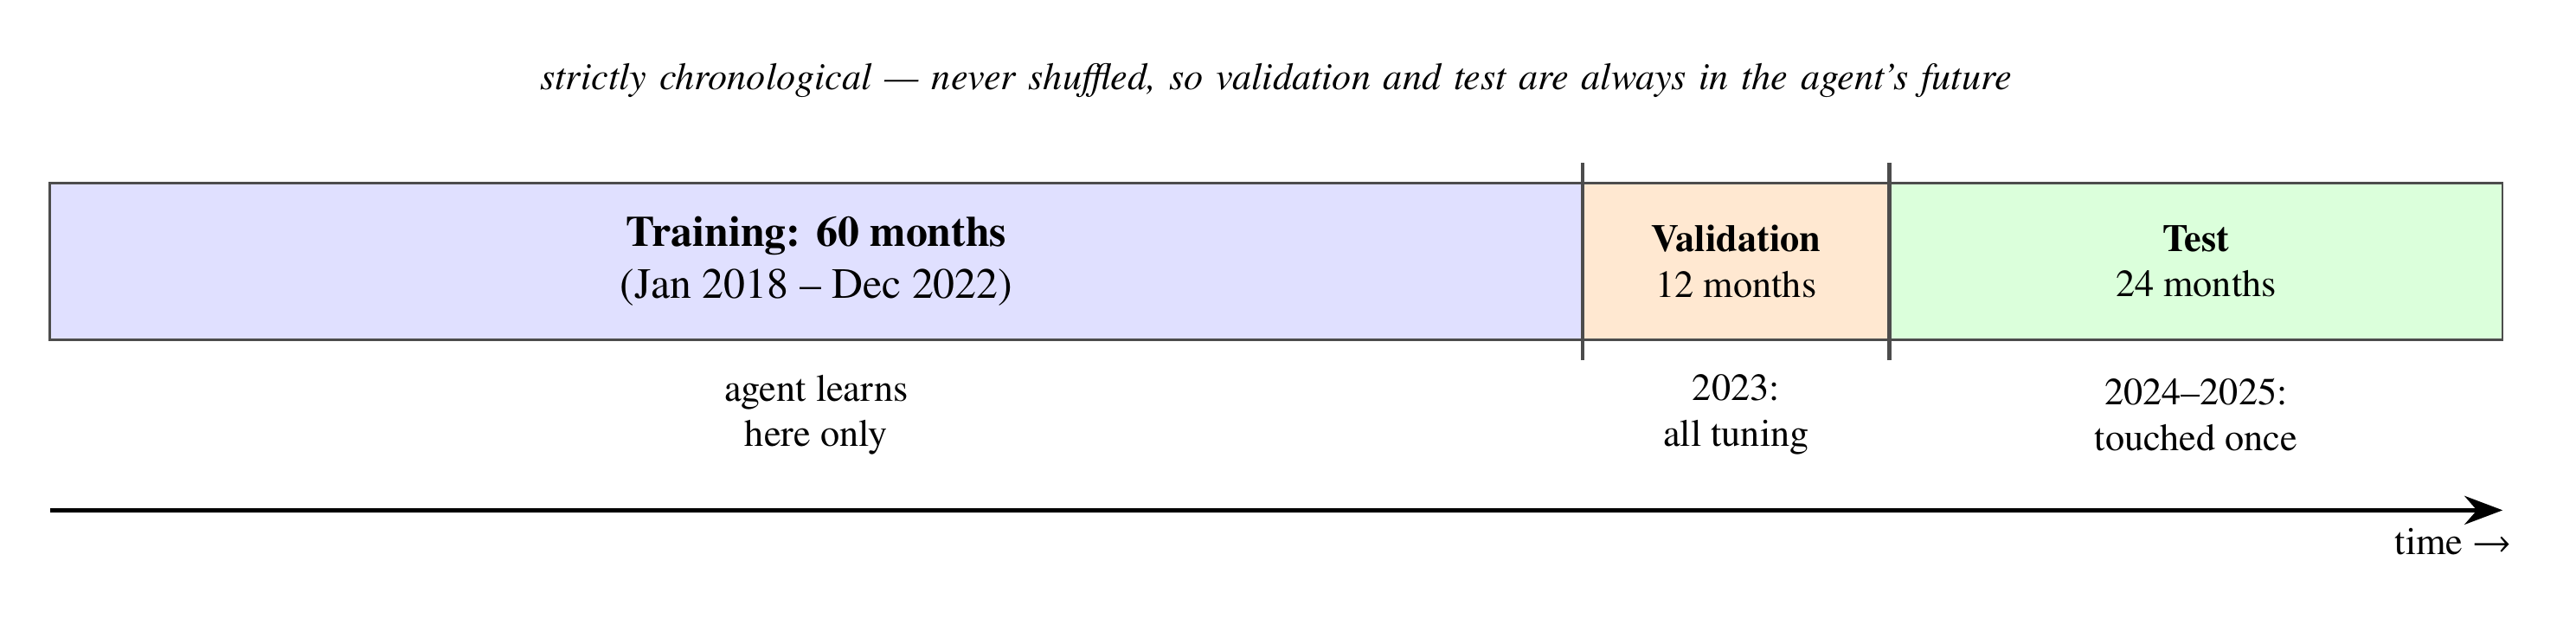
\includegraphics[width=0.9\textwidth]{media4/media/image1.png}
  \caption[Chronological split of the 96 monthly episodes]{Chronological split of the 96 monthly episodes: 60 training months, 12 validation months, and 24 held-out test months.}
\end{figure}


The episodes are kept in chronological order within the splits and are
not randomly shuffled between the three periods. The training set covers
January 2018 to December 2022 (60 monthly episodes) and is used to learn
the algorithms' parameters. The validation set covers 2023 (12 months)
and is used for decisions made during development, such as the fixed
trading amount. The test set contains the final 24 months, January 2024
to December 2025, and is kept separate from these decisions for only the
final evaluation.

Maintaining a chronological split is important for financial data~\cite{lopezdeprado2018}. This
prevents observations from later periods from entering the training set
and influencing the model's development. This would not reflect how a
trading strategy would be developed in practice.

The training period includes most market conditions, including the
volatility experienced in 2018, the COVID-19 market crash and recovery
in 2020, and the 2022 downtrend. The 2023 period is used for validation,
while 2024 and 2025 form the final test period.

The separation between validation and test data is especially important
for the experiments in Chapter 5. A configuration that performs well on
the validation period may therefore be selected to examine its
performance on the held-out test period. The test results are then used
to compare the learned strategies.

The processed episodes and their metadata are cached locally so that the
same dataset can be used consistently across all experiments.

\section{Training, Validation and Testing Procedure}

The experiments use a fixed sequence that separates training,
validation, and test periods. This separation ensures that the test data
are not used when making decisions about the model or experimental
setup.

\subsection{Training}

During training, each learning algorithm interacts with the monthly
episodes in the training period. Each algorithm is given the same market
data, state representation, portfolio conditions, and trading
constraints. The main difference between the algorithms is how they use
the collected experience to update their parameters.

REINFORCE updates the policy using the reward-to-go calculated from
completed monthly episodes. DQN updates its Q-network using transitions
sampled from the replay buffer. PPO collects fixed-length rollouts and
uses the resulting batches for several optimisation epochs.

Each configuration is trained using six random seeds. Using multiple
seeds reduces the dependence on using one particular network
initialisation or a sequence of sampled experiences and allows the variation between runs to be reported~\cite{henderson2018}.

The trained model from each seed is saved with its configuration so that
it can be evaluated later using the same settings.

\subsection{Validation}

The validation set contains the 12 monthly episodes from 2023.

This period is used for decisions that need to be made before the final
test. For example, it determines the fixed transaction amount traded for
each Buy or Sell action.

The candidate transaction sizes are 0.05, 0.10, 0.25, and 0.50 of the
initial capital.

The selection is based on the maximum portfolio exposure that can be
achieved from each action rather than on trading performance during the
test period. This prevents the action from being chosen simply because
it happens to perform well on the final evaluation data.

Once the required configuration decisions have been made, the selected
settings are fixed for testing.

\subsection{Testing}

The final evaluation uses the held-out data from January 2024 to
December 2025.

The test data are not used to make configuration decisions. This ensures
that results provide an independent assessment of the methods.

Each trained model is evaluated in the same trading environment and
using the same evaluation procedure, which includes the initial capital,
transaction costs, action constraints, and monthly episode structure.

For the learned agents, actions are selected intentionally by choosing
the highest-probability action for the policy-based methods or the
highest-valued action for DQN.

The portfolio outcomes are then recorded for each monthly test episode
and each random seed. This produces a consistent set of results that can
be used to compare the different learning algorithms.

The stored results therefore contain sufficient information to compare
algorithms, state representations, reward functions, and benchmark
strategies, which are presented in Chapter 5.

\section{Experiment Configuration}

The implementation was designed so that different experiments could be
run by changing their settings without changing the overall trading
environment or learning algorithm settings.

For this reason, experiments are defined through configuration files or
parameters rather than by manually changing the source code for each
run. Each experiment is therefore linked to a specific configuration
that records the conditions used to produce it.

This separates experiment settings from the environment's implementation
and learning algorithms, allowing the same code to run different state,
reward, and action configurations.

\subsection{Configuration Parameters}

The configuration records the main settings that can affect an
experiment\textquotesingle s outcome. These include:

\begin{itemize}
\item
  learning algorithm;
\item
  state representation and state dimensionality;
\item
  reward formulation;
\item
  transaction fee;
\item
  fixed transaction amounts;
\item
  risk-penalty coefficient, where applicable;
\item
  action model;
\item
  random seed;
\item
  training settings;
\item
  evaluation settings.
\end{itemize}

Using this approach reduces the need to manually change the source code
between experiments. It also makes the experimental process easier to
track, since each result can be linked directly to the configuration
that produced it.

This is particularly important for the experiments reported in Chapter
5, where several state, reward, and action configurations are compared.

\subsection{Algorithm Configuration}

The experiment uses the same starting capital and transaction cost
across all three learning algorithms. The initial capital is set to
\(C_{0} = \$ 10,000\), and a transaction fee of 0.05\% is applied to
each trade opened.

The main settings used for REINFORCE, DQN, and PPO are shown below.

{\def\LTcaptype{none} % do not increment counter
\begin{longtable}[]{@{}
  >{\centering\arraybackslash}p{(\linewidth - 6\tabcolsep) * \real{0.1885}}
  >{\centering\arraybackslash}p{(\linewidth - 6\tabcolsep) * \real{0.2837}}
  >{\centering\arraybackslash}p{(\linewidth - 6\tabcolsep) * \real{0.2699}}
  >{\centering\arraybackslash}p{(\linewidth - 6\tabcolsep) * \real{0.2501}}@{}}
\toprule\noalign{}
\begin{minipage}[b]{\linewidth}\centering
\textbf{Parameter}
\end{minipage} & \begin{minipage}[b]{\linewidth}\centering
\textbf{REINFORCE}
\end{minipage} & \begin{minipage}[b]{\linewidth}\centering
\textbf{DQN}
\end{minipage} & \begin{minipage}[b]{\linewidth}\centering
\textbf{PPO}
\end{minipage} \\
\midrule\noalign{}
\endhead
\bottomrule\noalign{}
\endlastfoot
Network & MLP with 2 hidden layers of 128

\(d \rightarrow 128 \rightarrow 128 \rightarrow 3\) & MLP with 2 hidden
layers of 128

\(d \rightarrow 128 \rightarrow 128 \rightarrow 3\) & \(MlpPolicy\)

\(d \rightarrow 128 \rightarrow 128\) \\
\rowsep
Activation & tanh & ReLU & \\
\rowsep
Optimiser & Adam & Adam & Adam \\
\rowsep
Learning rate & \(10^{- 3}\) & \(10^{- 3}\) & \({3*10}^{- 4}\) \\
\rowsep
Discount factor \(\gamma\) & 0.99 & 0.99 & 0.99 \\
\rowsep
Replay buffer & --- & 50,000 & --- \\
\rowsep
Batch size & Episode & 64 & 64 \\
\rowsep
Target network update & --- & Every 500 steps & --- \\
\rowsep
Exploration & Policy sampling & \(\epsilon - greedy\) & Policy
sampling \\
\rowsep
\(\epsilon\ schedule\) & --- & 1.0 → 0.05 & --- \\
\rowsep
PPO clipping & --- & --- & 0.2 \\
\rowsep
GAE & --- & --- & 0.95 \\
\rowsep
PPO epochs & --- & --- & 10 \\
\rowsep
Entropy coefficient & --- & --- & 0 \\
\rowsep
Training budget & 80,000 steps & 80,000 steps & 80,000 steps \\
\rowsep
Random seeds & 42--47 & 42--47 & 42--47 \\
\end{longtable}
}

All three methods use the same training budget of 80,000 steps and the
same six random seeds to keep the computational budget similar
throughout when comparing performance.

The experiments consider the different state and reward configurations
described in Chapter 5. These include the standard nine-feature state,
the ten-feature state with drawdown, the primary wealth-change reward,
the risk-aware reward, and the alternate action configurations.

The implementation also treats each trading position size as a
configurable parameter. Its final value is selected using the predefined
validation procedure. Chapter 5 reports the different values and their
effect on trading results as part of the experimental findings.

\subsection{Benchmark Implementation}

The learned agents are compared with benchmark strategies to provide
clear grounds for assessing their performance. These benchmarks are
simple trading behaviours that do not require reinforcement learning.

The main benchmark is a buy-and-hold strategy where the initial capital
is used to purchase the asset at the start of the episode. The position
is then held until the final trading step, when it is closed. The same
transaction fee and position closure used for the learned agents apply
to this benchmark.

This approach is different from gradually purchasing the asset using the
same fixed trade amount available to the learning agents. A gradual
purchasing strategy may take several trading days to build a position
and, if the fixed trade size is small, it may not become fully invested
before the monthly episode ends.

For this reason, the gradual purchase strategy is treated as a separate
reference strategy rather than as buy-and-hold. The conventional
buy-and-hold strategy gives the learned agents a straight performance
target.

The benchmark strategies use the same portfolio conditions, transaction
costs, and evaluation procedures as the learned agents. This keeps the
comparison consistent and reduces the chance that differences in results
stem from inaccuracies in calculating portfolio performance rather than
from the strategies themselves.

\section{Implementation Verifications}

Before using the experimental results for analysis, the implementation
was tested to ensure that it followed the definitions and constraints
established in Chapter 3.

These tests check that the environment, data pipeline, reward
calculation, and action constraints behave as intended.

The final implementation includes 21 automated tests covering all major
components, all of which pass. Appendix A lists every test and the
condition it verifies; this section summarises what each group of tests
protects.

\subsection{Environment and Portfolio Tests}

The environment tests focus on the correctness of the portfolio
calculations during trading.

The tests verify that portfolio wealth matches the cash balance and the
market value of current holdings. They also check that Buy and Sell
actions update the portfolio correctly and that transaction fees are
included in all transactions.

The tests further verify that invalid actions are handled correctly and
that each monthly episode ends without an open position.

These checks are important because an error in portfolio accounting
would affect the reported rewards and performance measures for all three
learning algorithms. Such an error could therefore lead to incorrect
conclusions even if the learning algorithms were implemented correctly.

\subsection{Feature and Data Tests}

The feature tests check that the state representation follows the
intended information structure defined in Chapter 3.

The tests verify that features do not use future information and that
rolling features access the necessary historical information when moving
from one monthly episode to the next. They also check that the state
dimensions and feature ordering match the reported configurations.

The chronological split is tested to ensure that the training,
validation, and test periods remain separate.

This testing process identified an important implementation issue. In an
earlier version of the pipeline, rolling features were recalculated
separately for each monthly episode, so the rolling windows restarted at
the beginning of every month instead of continuing from the previous
observations. This caused incomplete feature windows in approximately
\textbf{43.1\% of episode steps}. The correction --- calculating rolling
market features on the continuous dataset before dividing it into
monthly episodes --- is described with the other corrections in Section
4.6, and the corrected pipeline was tested again to confirm that
historical information is retained across episode boundaries.

\subsection{Reward and Risk Tests}

The reward tests verify that the primary wealth-change reward
corresponds to the change in portfolio wealth with no risk penalty
applied.

The risk-aware reward is tested separately to see whether increasing
drawdown does not lead to an increase in the reward due to the risk
penalty applied.

An additional test checks the relationship between the risk-aware reward
and the state representation. A risk-aware reward cannot be paired with
a state that does not have the drawdown feature.

The implementation uses this restriction so an inconsistent combination
of state and reward settings cannot run accidentally.

These tests therefore ensure that the relationship between state
representation and reward design described in Chapter 3 is also
maintained in the implemented system.

\subsection{Action-Masking Tests}

The action-masking tests verify that the environment correctly
identifies invalid actions that cannot be executed under the current
portfolio conditions.

The tests check that the Buy action is unavailable when the portfolio
has insufficient cash and that the Sell action is unavailable when the
agent does not hold enough of the asset. They also verify the different
configurable fixed trading amounts.

A defensive check is also included in the environment so that an invalid
action supplied externally is converted to Hold rather than being
executed.

Logs monitor these checks during the experiments. After the final
experiment, the recorded rate of invalid actions was zero during
evaluation, confirming that the action masks accurately prevented the
learning algorithms from executing any invalid trades during the testing
period.

\section{Implementation Corrections}

\subsection{Problems Identified During Development}

The verification process identified several implementation issues before
the final experiments were run.

The main issues involved the feature calculation, benchmark
implementation, and the risk-aware reward configuration.

First, the rolling market features using past observations did not
initially contain the needed historical context when a new monthly
episode began. These meant that some features were calculated using
shorter windows than intended.

Second, an earlier version of the buy-and-hold benchmark used the same
transaction size as the learning algorithms. This did not represent a
fully invested buy-and-hold strategy, where an asset is bought at the
beginning of an episode and held untouched till the end of the
experiment, and it caused understated exposure and benchmark
performance.

Third, the risk-aware reward could initially be used without requiring
the drawdown feature in the state. This created a mismatch between the
information needed by the reward and the information supplied to the
agent because drawdown information was unavailable.

These issues were treated as implementation errors that needed
correcting because leaving any of them in place would affect the
validity of comparisons between the learning algorithms and benchmark
strategies.

\subsection{Correction and Re-verification}

Each identified issue was addressed through a general correction
process:

\begin{enumerate}
\def\labelenumi{\arabic{enumi}.}
\item
  the problem was identified through testing or auditing the
  implementation;
\item
  its potential effect on the experiment results;
\item
  the relevant part of the implementation that needed correcting;
\item
  adding or updating verification tests where necessary after the
  correction;
\item
  completely running the verification tests again.
\end{enumerate}

The buy-and-hold issue, for example, shows why this process was
necessary. The affected implementation understated the benchmark by
approximately \textbf{\$38.95 per month}, or \textbf{21.6\%} before
correction.

These values describe only the incorrect implementation, which has been
discarded, and are reported here only to show the potential impact of
the error. They are not presented as findings about the
asset\textquotesingle s or the market\textquotesingle s performance.

After the corrections, the complete automated batch tests were run
again, and all 21 tests passed.

The final experiment results in Chapter 5 come only from the corrected
implementation, not the earlier incorrect versions.

\section{Complete Implementation Pipeline}

The complete implementation pipeline is a sequence of stages, from
collecting historical market data to storing the final evaluation test
results.

The first stage loads the SPY OHLCV data, including an initial warm-up
period needed to calculate the rolling features. The market features are
then calculated on the continuous dataset using only information
available up to said observation. Once feature construction is complete,
the data are divided chronologically into the training, validation, and
test datasets.

The observations are then grouped into monthly episodes. At the start of
each episode, the portfolio resets to the initial capital with no asset
holdings. At each timestep, the learning algorithm receives the current
state and selects one of the valid available actions. The trading
environment then executes the action with the transaction fee, updates
the portfolio, returns the reward, and moves to the next state.

REINFORCE, DQN, and PPO all interact with the same trading environment.
Their main difference is how each algorithm processes the experience to
update their model parameters.

After training and validation, the final experiment settings are fixed,
and the trained models are evaluated on the held-out 2024-2025 test
datasets. The resulting metrics, monthly results, training information,
configuration settings, and performance measures are stored together
with information about the software environment used to produce them.

This pipeline clearly links the methodological decisions defined in
Chapter 3, their implementation in the system, and the experiment
results presented in Chapter 5.

Figure 4.2 summarises the flow.

\begin{figure}[!htb]
  \centering
  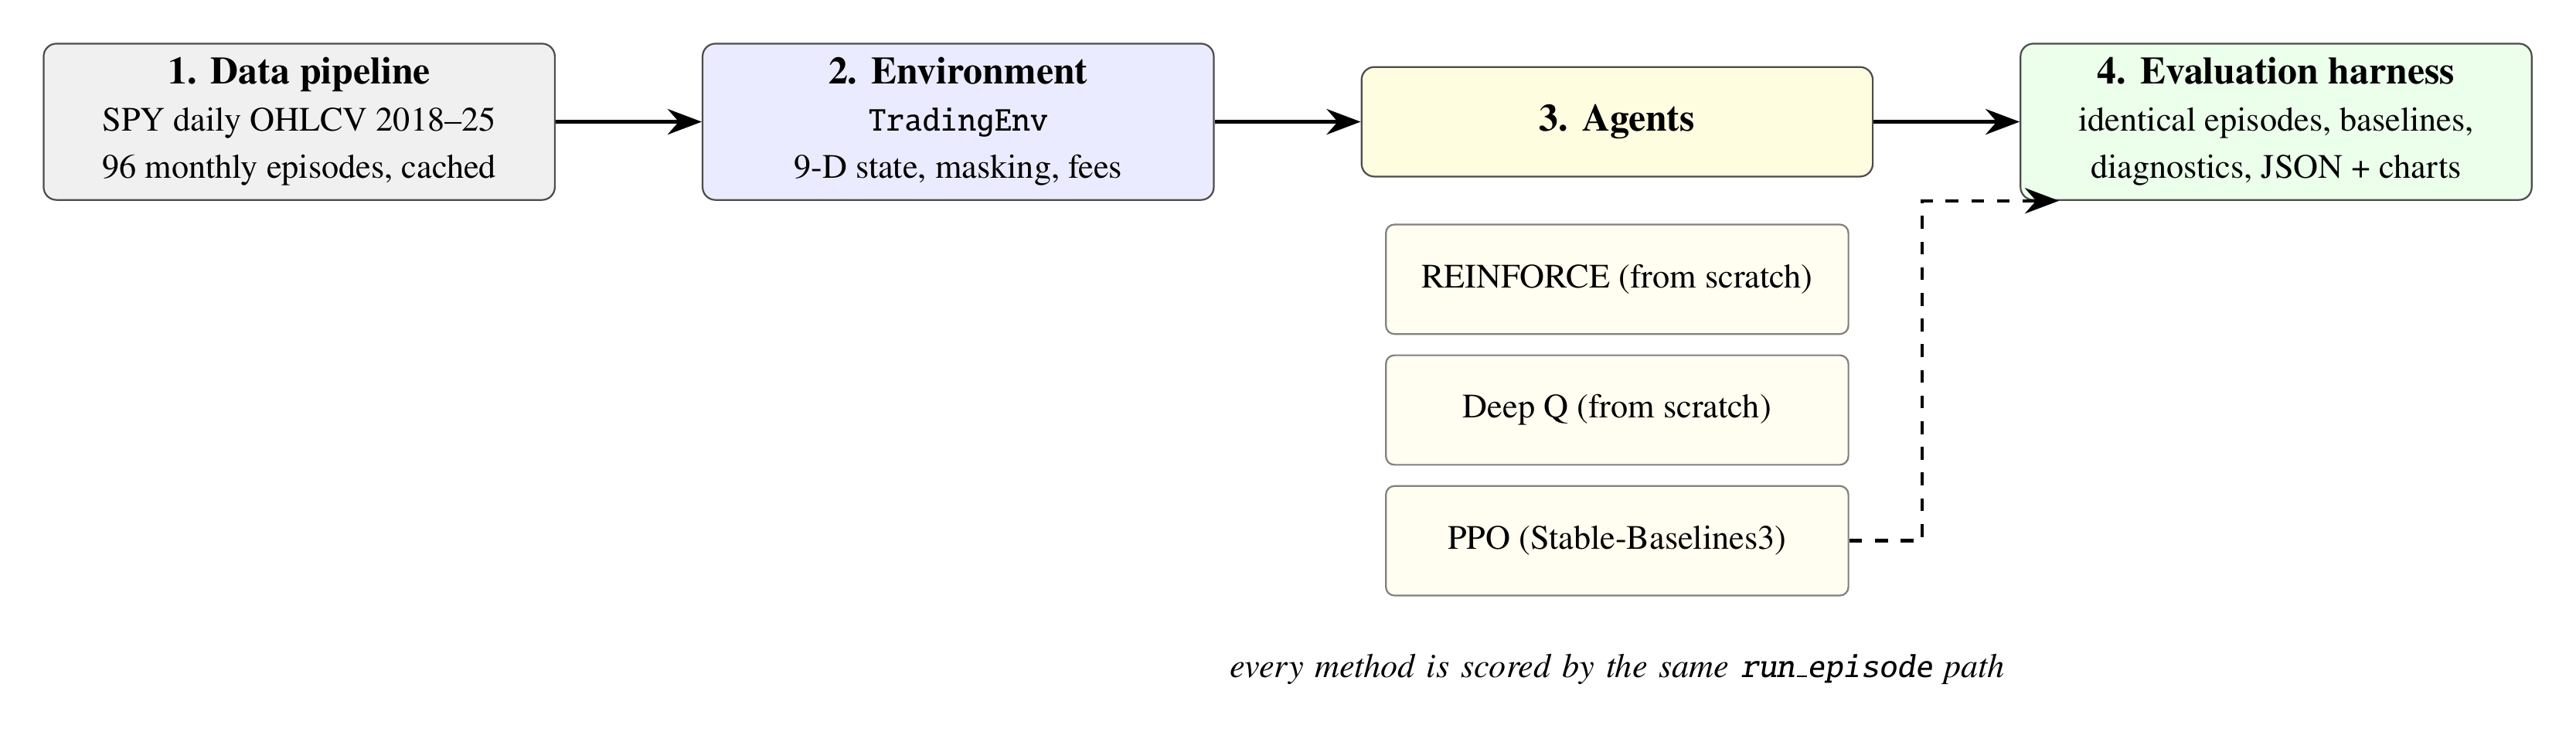
\includegraphics[width=0.9\textwidth]{media4/media/image2.png}
  \caption[System architecture showing the data flow described in Section 4.7.]{System architecture showing the data flow described in Section 4.7. All learned algorithms and benchmark strategies are evaluated using the same episode runner, ensuring that the comparison uses the same evaluation procedure\textbf{.}}
\end{figure}



\chapter{Experimental Results and Analysis}
\section{Introduction}

This chapter reports and analyses the experiment results from the
trading environment and learning algorithms described in Chapter 4. The
experiments examine the financial performance of the learned agents, the
effects of two state representations, and their respective reward
functions.

The experiments are structured around four questions that directly
relate to the objectives of the dissertation to increase portfolio
wealth:

\begin{enumerate}
\def\labelenumi{\arabic{enumi}.}
\item
  \textbf{Performance:} Do the learned agents outperform appropriate
  simple benchmarks on unseen data after accounting for transaction
  costs?
\item
  \textbf{Behaviour:} Do the learned agents make use of the market and
  portfolio information provided in the state representations?
\item
  \textbf{State representation:} Does adding the drawdown feature to the
  main nine-feature state affect the learned behaviour or financial
  performance?
\item
  \textbf{Reward:} Does the risk-aware reward improve the balance
  between return and drawdown, rather than simply encouraging the agent
  to trade less?
\end{enumerate}

A key part of the analysis is determining whether the learned strategies
outperform simple strategies. Buy-and-hold, for example, is an important
benchmark here. A learned agent producing a positive return does not
necessarily indicate that it has learned a useful trading strategy if a
simple investment strategy achieves a similar or better result.

For this reason, the analysis considers both \textbf{financial
performance} and \textbf{agent behaviour}. Financial performance is
evaluated using measures including wealth change, exposure, trading
activity, drawdown, and Sharpe ratio. Behavioural analysis examines
whether an agent\textquotesingle s actions change as the state changes.
This helps to identify a policy that responds to state information
rather than one that follows a fixed trading pattern.

\section{Experiment Protocols and Evaluation Criteria}

This section describes how the experiments in this chapter were
conducted and how the reported results should be interpreted.

\subsection{Experimental Configurations}

Each configuration trained REINFORCE, Deep Q-learning (DQN), and
Proximal Policy Optimisation (PPO) separately for 80,000 steps per seed
in the portfolio environment,

To account for randomness in reinforcement learning~\cite{henderson2018}, six random seeds
were used, with an initial capital of \(C_{0} = \$ 10,000\) at the start
of every monthly episode. This means six independent training runs all
with the same configuration, allowing us to analyse the consistency of
each algorithm's results rather than relying on a single training run.

During evaluation, all policies acted deterministically: policy-gradient
algorithms select the action with the highest probability, while
value-based algorithms select the action with the highest estimated
value.

The 2023 validation period was used to make every experimental decision
reported in this chapter. This included selecting the trade size in
Section 5.3, the risk-penalty weight in Section 5.7, and the transaction
fee in Section 5.8. These choices were fixed before using them for the
main experiments in the 24 held-out test months from 2024--2025.

There are three main learned experiments in this chapter:

\begin{itemize}
\item
  The primary experiment evaluating the nine-feature state with the
  wealth-change reward.
\item
  The ten-feature state that adds drawdown while keeping the same
  wealth-change reward.
\item
  The third experiment using the ten-feature state with the risk-aware
  reward, which actually requires drawdown.
\end{itemize}

\subsection{Evaluation Metrics}

There are five financial measures used in each experiment report. They
are averaged over the episodes and, for learned agents, across the six
training seeds:

\begin{itemize}
\item
  Mean wealth change \((\Delta W)\) reported in dollars per month;
\item
  Mean exposure \((\Delta v_{t})\), which represents the proportion of
  initial capital invested in the asset and is averaged across trading
  days;
\item
  Trades per month;
\item
  Mean episode drawdown \((\Delta{dd}_{t})\);
\item
  and the monthly Sharpe ratio~\cite{sharpe1994}, a financial metric that calculates the
  average return relative to the variation of those daily returns during
  the month.
\end{itemize}

The tables also report the \textbf{seed spread}, which is the difference
between the best and worst result across the six seeds. This is included
because there might be large differences between training runs which the
average alone may hide~\cite{henderson2018}. A large spread indicates that the algorithm did
not produce a consistent trading behaviour across the different runs.

Financial performance is then followed by a behavioural analysis, as
returns alone cannot show whether a policy actually used the information
in its state. For example, a policy that buys simply because buying is
allowed can perform well during a rising market without responding to
any market information.

This led to \textbf{state-dependence analysis,} which was used to test
whether a policy\textquotesingle s actions changed when its observed
state changed while the valid actions remained the same. For instance,
if a policy selected different actions at different steps with the same
actions available, the difference could be attributed to the observed
state. The tables report how many of the six seeds met this condition.

\subsection{Benchmark Strategies}

Two non-learning strategies are used as benchmarks. They use the same
trading environment, portfolio conditions, and transaction fees as the
learned agents.

\textbf{Buy-and-hold} invests the full initial capital on the first
trading day and holds the position until the end of the month, when the
position is closed. This is the main benchmark as it is a simple passive
investment strategy.

\textbf{Always-buy} \(\mathbf{(0.25}\mathbf{C}_{\mathbf{0}}\mathbf{)}\)
purchases a fixed trade amount equal to 25\% of the initial capital
whenever buying is available, continuing until it has fully invested in
that asset. This strategy is useful for comparing against policies that
achieve their returns through repeated buying rather than by using
information from its observed state, as it also does not use any market
or portfolio information when deciding whether to buy.

\section{Fixed Trade Size Tuning}

Before comparing the learned agents with the benchmarks, the fixed
transaction size used by the learning agents must be finalized.
Determining this trading-action size matters because the amount traded
at each decision point determines how quickly the agent can build or
reduce its position during a monthly episode.

In the trading environment, each Buy or Sell action changes the trade by
a fixed fraction of the initial capital. A smaller value gives the agent
finer control over its position but also means that more trading
decisions are needed to reach a high level of asset exposure. A larger
value lets the agent build its position more quickly but provides less
control over the size of each change.

This creates a problem between the learned agents and the buy-and-hold
benchmark. Buy-and-hold invests the available capital at the beginning
of the episode, while a trading agent must build its position through
repeated actions. If the trade size uses a small, fixed transaction
size, the agent will need several trading days to reach a similar
exposure as buy-and-hold and may not overall reach the same exposure
within a typical month. Poor results could therefore arise from the
fixed trade amounts rather than from the learned policy.

The trade size was therefore calibrated using the validation data to
select the most stable size before running the main comparison between
learning algorithms on the held-out data.

\subsection{Exposure available under different transaction sizes}

The validation experiment measures the maximum exposure reachable during
a month using a policy that always buys whenever the action is
available, for each fixed transaction size. The validation set contains
12 monthly episodes, with an average length of approximately 20.8
trading days. Table 5.1 and Figure 5.1 show the results.

\addcontentsline{lot}{table}{\protect\numberline{5.1}{Attainable exposure for each fixed trade amount on the validation months. The policy buys whenever a purchase is valid.}}
\emph{Table 5.1: Attainable exposure for each fixed trade amount on the
validation months. The policy buys whenever a purchase is valid.}

{\def\LTcaptype{none} % do not increment counter
\begin{longtable}[]{@{}
  >{\centering\arraybackslash}p{(\linewidth - 6\tabcolsep) * \real{0.1725}}
  >{\centering\arraybackslash}p{(\linewidth - 6\tabcolsep) * \real{0.3929}}
  >{\centering\arraybackslash}p{(\linewidth - 6\tabcolsep) * \real{0.2374}}
  >{\centering\arraybackslash}p{(\linewidth - 6\tabcolsep) * \real{0.1973}}@{}}
\toprule\noalign{}
\begin{minipage}[b]{\linewidth}\centering
\textbf{Trade amount}
\end{minipage} & \begin{minipage}[b]{\linewidth}\centering
\textbf{Buys Days required to purchase a full asset}
\end{minipage} & \begin{minipage}[b]{\linewidth}\centering
\textbf{Mean maximum exposure}
\end{minipage} & \begin{minipage}[b]{\linewidth}\centering
\textbf{Mean wealth change}
\end{minipage} \\
\midrule\noalign{}
\endhead
\bottomrule\noalign{}
\endlastfoot
0.05C₀ & 20 & 0.450 & +\$95.49 \\
\rowsep
0.10C₀ & 10 & 0.690 & +\$121.79 \\
\rowsep
0.25C₀ & 4 & 0.838 & +\$167.39 \\
\rowsep
0.50C₀ & 2 & 0.886 & +\$162.77 \\
\rowsep
Buy-and-hold & --- & 0.910 & +\$166.92 \\
\end{longtable}
}

\begin{figure}[!htb]
  \centering
  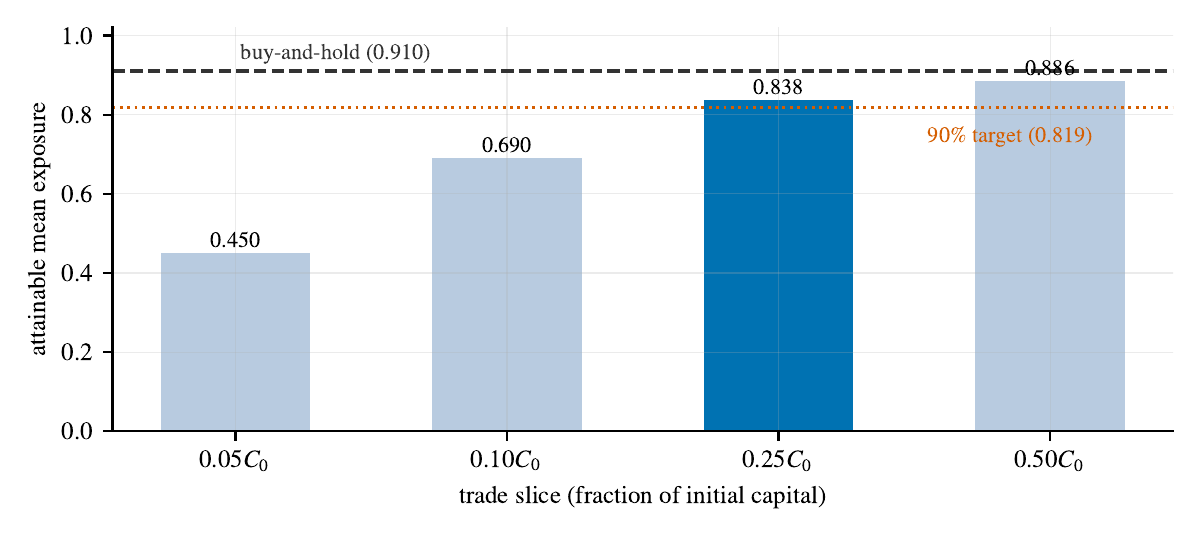
\includegraphics[width=0.9\textwidth]{media4/media/image3.png}
  \caption[Exposure ceilings from Table 5.1.]{Exposure ceilings from Table 5.1. The 0.25 C₀ trade amount (highlighted) is the smallest that clears the 90\% target of buy-and-hold's exposure; the 0.10 C₀ amount cannot reach it even in principle.}
\end{figure}


The results show that the original\(\ 0.10C₀\) trade size restricts the
agent\textquotesingle s asset exposure. This trade size requires ten buy
days to fully invest in that asset, but the average episode is only 20.8
trading days long, so half a typical month passes before full investment
is even possible.~ Its mean maximum exposure is 0.690, which is also
significantly below the 0.910 asset exposure for the simple buy-and-hold
strategy.

Hence, even a policy that buys whenever possible cannot reach the same
level of exposure as a simple benchmark during a typical monthly
episode. This matters when analysing the agent's performance. A low
return may result from poor decision-making, but it may also result from
the trading size preventing the agent from investing enough in the
asset. The two outcomes should be treated distinctly.

The \(\ 0.25C₀\) trade size was therefore selected as the primary
configuration, reaching 0.838 exposure, which corresponds to
approximately 92\% of the buy-and-hold exposure. This selection was
based on the criteria that exposure must reach at least 90\% of the
buy-and-hold, since no trade size can reach that level completely.

The buy-and-hold exposure of 0.910 gives an average exposure of
approximately 0.819 under this criterion. The \(0.25C₀\) trade size
therefore satisfies the requirement as the smallest tested trade size
whose exposure is close to the benchmark.

Increasing the trade size setting to \(0.50C₀\) raises exposure
slightly, from 0.838 to 0.886, but makes each individual action much
larger, giving the agent less control over gradual exposure changes.

Based on this calibration, the \(0.25C₀\) size balances maximum asset
exposure and control over position changes. It gives the learned agents
a reasonable opportunity to reach the benchmark level without using a
much coarser \(0.50C₀\) trade size.

\section{Do the Learned Policies Use Their Observations?}

The Financial performance of the portfolio trading agent on its own does
not show whether a learned agent is actually using the information
contained in its state representation. For example, an agent that buys
whenever buying is possible can perform well in a rising market without
using any of the market information its state provides.

This requires examining the behavioural patterns of the agents' learned
strategies to identify whether a policy selects a different action when
the state changes, provided the available valid actions remain the same.
This shows that the policy responds to its observed state rather than
simply following action constraints and can be classified as
\textbf{state-dependent.}

The experiment is performed on the validation data using the calibrated
\(0.25C₀\) trade size decided in Section 5.3, with the nine-feature
state and the primary wealth-change reward. This test aims only to
analyse behavioural differences between the algorithms by determining
whether changes in the information provided to the agent are reflected
in its decisions. It is not used to determine the final financial
performance of the agents.

Every cell was trained from scratch for this study: six seeds per
method, 80,000 steps each.

\subsection{Behaviour of the learned policies}

\addcontentsline{lot}{table}{\protect\numberline{5.2}{Behavioural Results on the validation months (0.25 C₀ trade size, nine-feature state, wealth-change reward, six freshly trained seeds). The always-buy strategy shows the maximum asset exposure this trade size can reach.}}
\emph{Table 5.2: Behavioural Results on the validation months (0.25 C₀
trade size, nine-feature state, wealth-change reward, six freshly
trained seeds). The always-buy strategy shows the maximum asset exposure
this trade size can reach.}

{\def\LTcaptype{none} % do not increment counter
\begin{longtable}[]{@{}
  >{\raggedright\arraybackslash}p{(\linewidth - 10\tabcolsep) * \real{0.1676}}
  >{\centering\arraybackslash}p{(\linewidth - 10\tabcolsep) * \real{0.1665}}
  >{\centering\arraybackslash}p{(\linewidth - 10\tabcolsep) * \real{0.1664}}
  >{\centering\arraybackslash}p{(\linewidth - 10\tabcolsep) * \real{0.1666}}
  >{\centering\arraybackslash}p{(\linewidth - 10\tabcolsep) * \real{0.1663}}
  >{\centering\arraybackslash}p{(\linewidth - 10\tabcolsep) * \real{0.1667}}@{}}
\toprule\noalign{}
\begin{minipage}[b]{\linewidth}\centering
\textbf{Policy}
\end{minipage} & \begin{minipage}[b]{\linewidth}\centering
\textbf{Mean ΔW}
\end{minipage} & \begin{minipage}[b]{\linewidth}\centering
\textbf{Seed spread}
\end{minipage} & \begin{minipage}[b]{\linewidth}\centering
\textbf{Exposure}
\end{minipage} & \begin{minipage}[b]{\linewidth}\centering
\textbf{Trades}
\end{minipage} & \begin{minipage}[b]{\linewidth}\centering
\textbf{State-dependent}
\end{minipage} \\
\midrule\noalign{}
\endhead
\bottomrule\noalign{}
\endlastfoot
\textbf{Always-buy} & +\$167.39 & --- & 0.838 & --- & --- \\
\rowsep
\textbf{REINFORCE} & +\$154.96 & \$37.29 & 0.807 & 10.3 & 0/6 \\
\rowsep
\textbf{Deep Q-learning} & +\$86.16 & \$64.20 & 0.325 & 8.5 & 6/6 \\
\rowsep
\textbf{PPO} & +\$118.55 & \$167.39 & 0.596 & 3.7 & 0/6 \\
\end{longtable}
}

\begin{figure}[!htb]
  \centering
  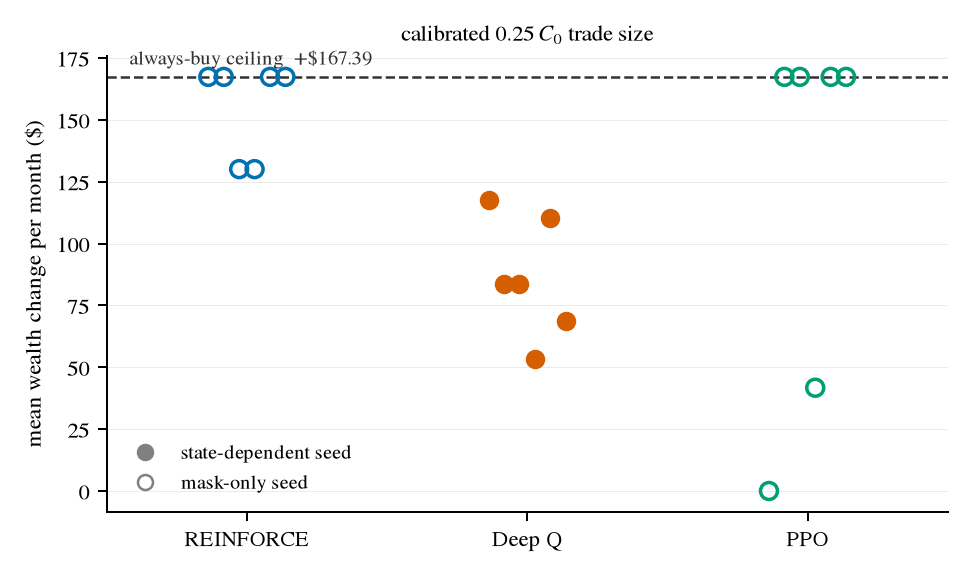
\includegraphics[width=0.9\textwidth]{media4/media/image4.png}
  \caption[Results for each seed from Table 5.2.]{Results for each seed from Table 5.2. Hollow-marker seeds show actions that don't depend on their state information; filled-marker seeds are state-dependent ones. Policy-gradient methods (REINFORCE, PPO) produce policies that cluster to either high exposure or collapse towards zero, while all six Deep Q-learning seeds fall between those corners.}
\end{figure}


Table 5.2 summarises the outcome and Figure 5.2 shows every seed
individually. The columns read as follows. Mean ΔW is the average wealth
change per month, calculated over the 12 validation months and then over
the six seeds. Seed spread is the difference between the best and worst
seeds; a spread larger than the mean produced noticeably different
results and did not agree on a strategy. State-dependent counts how many
of the six seeds act according to the experimental behaviour being
analysed.

The REINFORCE results are clearer when the individual seeds are read.
Four of its six seeds finished at exactly +\$167.39 with an exposure of
0.838. This matches the always-buy strategy, which was set as the upper
limit. These policies buy on the first four days when buying is valid,
hold the position, and close at the end of the month. The other two
seeds earned +\$130.10 while trading 20.8 times per month: Their actions
followed a fixed pattern of trading on each bar rather than changing in
response to the market state.

PPO produced three different behaviours across its six seeds. Four seeds
reached the always-buy result of +\$167.39. One seed never traded at
all, producing a wealth change of \$0.00 and an exposure of 0.000. The
remaining seed earned +\$41.73, relying on only two trading styles. This
produced a seed spread of \$167.39, showing the large difference between
the strongest and weakest PPO runs.

Deep Q-learning is the only method where none of its seeds reached
either extreme behaviours, unlike the policy-gradient methods. Its
results ranged from +\$53.23 to +\$117.43, with a mean wealth change of
+\$86.16 and an average exposure of 0.325, less than half the 0.838
standard exposure of the always-buy strategy.

\subsection{State-dependence analysis}

The final column in Table 5.2 summarises the state-dependence test, with
the count representing the difference in behaviour across the six seeds

For REINFORCE, the result of 0/6 means that none of the six
independently trained policies changed their action when the state
changed while the same actions remained valid. The four seeds that
reached the maximum exposure followed the same basic rule of buying
whenever possible, while the other two followed a fixed trading pattern.
The diagnostic therefore found no evidence that these policies used
market and portfolio features to change their decisions.

Deep Q-learning produced the opposite result. All six seeds were
classified as state-dependent. Each seed selected different actions in
states where the same valid actions were available. This indicates that
the observed current state influences the decisions made by the DQN
policies.

PPO produced the same result as REINFORCE, with 0/6 state-dependent
seeds. Taken together, the splits are categorical by algorithm family
across the three methods: all six DQN seeds were state-dependent,
compared with none of the 12 policy-gradient seeds from REINFORCE and
PPO.

\subsection{Interpretation of the learned trading behaviour}

The different results across the three methods suggest that the learning
approach had a strong influence on the type of trading behaviour that
developed. REINFORCE and PPO frequently moved towards simple policies
that did not change their actions in response to the observed state,
whereas Deep Q-learning showed state-dependent behaviour across all six
seeds.

One possible explanation is the difference between policy-gradient and
value-based learning. REINFORCE updates the probability of an action
according to the return that follows it. When the market generally
favours holding an asset, repeatedly buying can produce a strong return
without needing to sample other policies. The learning signal may
therefore settle on a simple high-exposure strategy for higher rewards
rather than exploring.

PPO uses a different update rule from REINFORCE, but it still learns a
policy directly. Its clipped objective prevents large policy changes,
which can make learning more stable, but it does not need the policy to
become state-dependent. If a simple trading rule produces consistently
positive returns, the policy may face little pressure to learn a more
complex relationship between state and action. The extreme seed outcomes
are what hint at this. Seeds from both policy-gradient methods finish at
the always-buy upper limit, since that is the most rewarding.

Deep Q-learning learns differently. Rather than adjusting action
probabilities directly, it estimates the value of each available action
in the current state and picks the action with the highest estimate at
each step. When future estimated values differ, the chosen action
changes accordingly, and the agent has to distinguish between these
actions. The state-dependent behaviour therefore becomes a structural
property of this algorithm rather than an achievement, as it necessarily
depends on the changes in the market and portfolio state.

These explanations should be treated as interpretations of observed
behaviours rather than as direct evidence of the internal learning
process. This experiment was not designed to find out the precise reason
the algorithms moved to these different strategies. They are, however,
consistent, as different seeds show that learning algorithms affect how
available state information is used to develop a trading strategy.

\section{Effect of the State Representation}

Chapter 3 defines the nine-feature state as the main state
representation used in this study. It includes market, portfolio,
position, and time information. Drawdown is intentionally treated
separately as an additional risk-related feature rather than as the last
stage of the state design.

This experiment therefore focuses on a specific question: does adding
drawdown to the nine-feature state produce a meaningful change in
performance or behaviour when the reward function remains unchanged?

The comparison keeps the following conditions fixed:

\begin{itemize}
\item
  The same wealth-change reward;
\item
  the same \(0.25C₀\) trade size;
\item
  the same held-out test period;
\item
  the same six random seeds.
\end{itemize}

The intended difference between the two configurations is therefore only
the inclusion of drawdown in the state.

\subsection{Nine-Feature vs Ten-Feature State}

{\def\LTcaptype{none} % do not increment counter
\begin{longtable}[]{@{}
  >{\raggedright\arraybackslash}p{(\linewidth - 16\tabcolsep) * \real{0.1541}}
  >{\centering\arraybackslash}p{(\linewidth - 16\tabcolsep) * \real{0.1241}}
  >{\centering\arraybackslash}p{(\linewidth - 16\tabcolsep) * \real{0.1018}}
  >{\centering\arraybackslash}p{(\linewidth - 16\tabcolsep) * \real{0.0952}}
  >{\centering\arraybackslash}p{(\linewidth - 16\tabcolsep) * \real{0.1213}}
  >{\centering\arraybackslash}p{(\linewidth - 16\tabcolsep) * \real{0.0890}}
  >{\centering\arraybackslash}p{(\linewidth - 16\tabcolsep) * \real{0.0876}}
  >{\centering\arraybackslash}p{(\linewidth - 16\tabcolsep) * \real{0.0952}}
  >{\centering\arraybackslash}p{(\linewidth - 16\tabcolsep) * \real{0.1318}}@{}}
\toprule\noalign{}
\begin{minipage}[b]{\linewidth}\centering
\textbf{Method}
\end{minipage} & \begin{minipage}[b]{\linewidth}\centering
\textbf{State}
\end{minipage} & \begin{minipage}[b]{\linewidth}\centering
\textbf{ΔW (\$)}
\end{minipage} & \begin{minipage}[b]{\linewidth}\centering
\textbf{Spread}
\end{minipage} & \begin{minipage}[b]{\linewidth}\centering
\textbf{Exposure}
\end{minipage} & \begin{minipage}[b]{\linewidth}\centering
\textbf{Trades}
\end{minipage} & \begin{minipage}[b]{\linewidth}\centering
\textbf{DD}
\end{minipage} & \begin{minipage}[b]{\linewidth}\centering
\textbf{Sharpe}
\end{minipage} & \begin{minipage}[b]{\linewidth}\centering
\textbf{State-dep.}
\end{minipage} \\
\midrule\noalign{}
\endhead
\bottomrule\noalign{}
\endlastfoot
\textbf{REINFORCE} & 9-feature & +171.51 & 24.7 & 0.810 & 10.3 & 0.0266
& 0.675 & 0/6 \\
\rowsep
\textbf{REINFORCE} & 10-feature & +167.39 & 24.7 & 0.794 & 13.0 & 0.0263
& 0.670 & 0/6 \\
\rowsep
\textbf{Deep Q} & 9-feature & +74.68 & 71.4 & 0.312 & 8.2 & 0.0124 &
0.507 & 6/6 \\
\rowsep
\textbf{Deep Q} & 10-feature & +77.81 & 89.5 & 0.354 & 7.4 & 0.0140 &
0.505 & 6/6 \\
\rowsep
\textbf{PPO} & 9-feature & +127.35 & 179.8 & 0.598 & 3.7 & 0.0195 &
0.562 & 0/6 \\
\rowsep
\textbf{PPO} & 10-feature & +159.97 & 94.0 & 0.759 & 7.3 & 0.0250 &
0.671 & 1/6 \\
\end{longtable}
}

\addcontentsline{lot}{table}{\protect\numberline{5.3}{Results of the nine- and ten-feature states on the test data (wealth-change reward, 0.25 C₀ trade size, six seeds). DD shows the mean drawdown within each episode, while State-dep. shows the number of seeds where actions changed with the observed state.}}
\emph{Table 5.3: Results of the nine- and ten-feature states on the test
data (wealth-change reward, 0.25 C₀ trade size, six seeds). DD shows the
mean drawdown within each episode, while State-dep. shows the number of
seeds where actions changed with the observed state.}

The effect of adding drawdown and the changes in mean wealth performance
for REINFORCE and DQN are small.

For REINFORCE, wealth change falls from \$171.5 with the nine-feature
state to +\$167.39 with the ten-feature state. The difference is only
−\$4.12 per month against a seed spread of \$24.70 for both
configurations, which is considerably larger than the mean wealth
change.

The behavioural result also remains unchanged. None of the six seeds are
classified as state-dependent in either configuration. Adding drawdown
therefore did not produce a noticeable change in the behaviour of the
REINFORCE policies.

DQN shows a small change in the opposite direction. Wealth increases
from +\$74.68 to +\$77.81, a change of +\$3.13 per month. The seed
spreads are \$71.40 and \$89.50, respectively, so the change between the
two state configurations is again much smaller than the variation across
seeds.

The behavioural result is unchanged for DQN. All six seeds remain
state-dependent with both state representations.

PPO appears to improve, from +\$127.35 to +\$159.97, gaining \$32.62.
However, the result needs to be considered alongside the variation
between seeds. The nine-feature configuration has a spread of
\$179.80---larger than the mean itself --- but it narrows to \$94.00 in
the ten-feature configuration, with only one seed becoming
state-dependent.

The change in the mean is therefore not enough, on its own, to show that
adding drawdown caused the improvement.

\subsection{Analysis When Drawdown Was Added}

The other performance measures columns tell the same story in different
parts. For DQN, average exposure rose from 0.312 to 0.354, and mean
drawdown from 0.0124 to 0.0140 after adding that feature to the state
--- return, exposure, and risk all moved up together by similar
proportions. Its Sharpe ratio, however, changes very little, from 0.507
to 0.505.

The patterns noticed here suggest the additional drawdown feature did
not lead to more effective risk-aware decisions, but to slightly larger
asset exposure

The changes for REINFORCE barely move. Exposure falls from 0.810 to
0.794, while drawdown decreases slightly from 0.0266 to 0.0263, as
expected of a policy algorithm that does not read the state it is given.

The small changes in the financial measures therefore do not indicate a
change in the basic policy behaviour.

Overall, the results do not show a consistent improvement in either
performance or behaviour from adding drawdown to the state while using
the default wealth-change reward.

\subsection{Interpretation}

These results do not mean that drawdown information is unimportant. They
show that, in this environment, without changing the reward objective,
the additional information did not provide a clear advantage--- an agent
maximising wealth change in general rising markets has little use for
its own loss history.

This matters because Chapter 3 introduced drawdown to provide
information that could support risk-sensitive decisions. However, this
feature becomes relevant only when the agent's learning objective makes
larger drawdowns costly while increasing portfolio wealth, which is
precisely what the risk-aware reward experiment in Section 5.7 tests.

\section{Held-Out Test Results}

The main performance question of how each learned strategy, in its final
configuration, compares with the simple benchmarks on unseen data is
evaluated on the 24 held-out months from January 2024 to December 2025.

At this point, the main configuration has been fixed:

\begin{itemize}
\item
  nine-feature state;
\item
  wealth-change reward;
\item
  \(0.25C₀\) trade size;
\item
  0.05\% transaction fee;
\item
  six random seeds.
\end{itemize}

\subsection{Overall Comparison with the Benchmark Strategies}

{\def\LTcaptype{none} % do not increment counter
\begin{longtable}[]{@{}
  >{\raggedright\arraybackslash}p{(\linewidth - 14\tabcolsep) * \real{0.1676}}
  >{\centering\arraybackslash}p{(\linewidth - 14\tabcolsep) * \real{0.1210}}
  >{\centering\arraybackslash}p{(\linewidth - 14\tabcolsep) * \real{0.1177}}
  >{\centering\arraybackslash}p{(\linewidth - 14\tabcolsep) * \real{0.1364}}
  >{\centering\arraybackslash}p{(\linewidth - 14\tabcolsep) * \real{0.1146}}
  >{\centering\arraybackslash}p{(\linewidth - 14\tabcolsep) * \real{0.1139}}
  >{\centering\arraybackslash}p{(\linewidth - 14\tabcolsep) * \real{0.1177}}
  >{\centering\arraybackslash}p{(\linewidth - 14\tabcolsep) * \real{0.1111}}@{}}
\toprule\noalign{}
\begin{minipage}[b]{\linewidth}\centering
\textbf{Policy}
\end{minipage} & \begin{minipage}[b]{\linewidth}\centering
\textbf{ΔW (\$)}
\end{minipage} & \begin{minipage}[b]{\linewidth}\centering
\textbf{Spread}
\end{minipage} & \begin{minipage}[b]{\linewidth}\centering
\textbf{Exposure}
\end{minipage} & \begin{minipage}[b]{\linewidth}\centering
\textbf{Trades}
\end{minipage} & \begin{minipage}[b]{\linewidth}\centering
\textbf{DD}
\end{minipage} & \begin{minipage}[b]{\linewidth}\centering
\textbf{Sharpe}
\end{minipage} & \begin{minipage}[b]{\linewidth}\centering
\textbf{State-dep.}
\end{minipage} \\
\midrule\noalign{}
\endhead
\bottomrule\noalign{}
\endlastfoot
\textbf{Buy-and-hold} & +180.25 & --- & 0.913 & 2.0 & 0.0310 & 0.638 &
--- \\
\rowsep
\textbf{Always-buy (}\(\mathbf{0.25}\mathbf{C₀}\)\textbf{)} & +179.75 &
--- & 0.841 & 5.0 & 0.0274 & 0.684 & --- \\
\rowsep
\textbf{REINFORCE} & +171.51 & 24.7 & 0.810 & 10.3 & 0.0266 & 0.675 &
0/6 \\
\rowsep
\textbf{Deep Q-learning} & +74.68 & 71.4 & 0.312 & 8.2 & 0.0124 & 0.507
& 6/6 \\
\rowsep
\textbf{PPO} & +127.35 & 179.8 & 0.598 & 3.7 & 0.0195 & 0.562 & 0/6 \\
\end{longtable}
}

\addcontentsline{lot}{table}{\protect\numberline{5.4}{test results over the 24 held-out months (2024--2025): benchmarks and the three learned agents in their final configuration, six seeds each.}}
\emph{Table 5.4: test results over the 24 held-out months (2024--2025):
benchmarks and the three learned agents in their final configuration,
six seeds each.}

Table 5.4 is the central result of this dissertation.

Two simple strategies are used as benchmarks. Buy-and-hold invests the
full capital on the first day and is the benchmark an investor would
actually compare against. Always-buy at \(0.25C₀\) buys an asset at a
quarter fraction of the initial capital. This takes trades with every
valid action until it has fully invested in the asset. It represents a
strategy that buys unconditionally at the fixed trade size, without
requiring observations.

The central result is straightforward: none of the three learned agents
outperformed buy-and-hold during the held-out test period.

Buy-and-hold earned +\$180.25 per month, equivalent to a 1.8025\%
increase of the initial capital per monthly episode, and no learned
agent reached this. The closest was REINFORCE at +\$171.51, which was
\$8.74 short of buy-and-hold per month; PPO earned +\$127.35 and Deep
Q-learning +\$74.68.

Always buying at \(0.25C₀\) earned +\$179.75, within \$0.50 of
buy-and-hold, and it sets the standard a learned agent must reach/beat
before it can claim any skill, as matching it needs no market
information at all --- only buying whenever buying is available.

\begin{figure}[!htb]
  \centering
  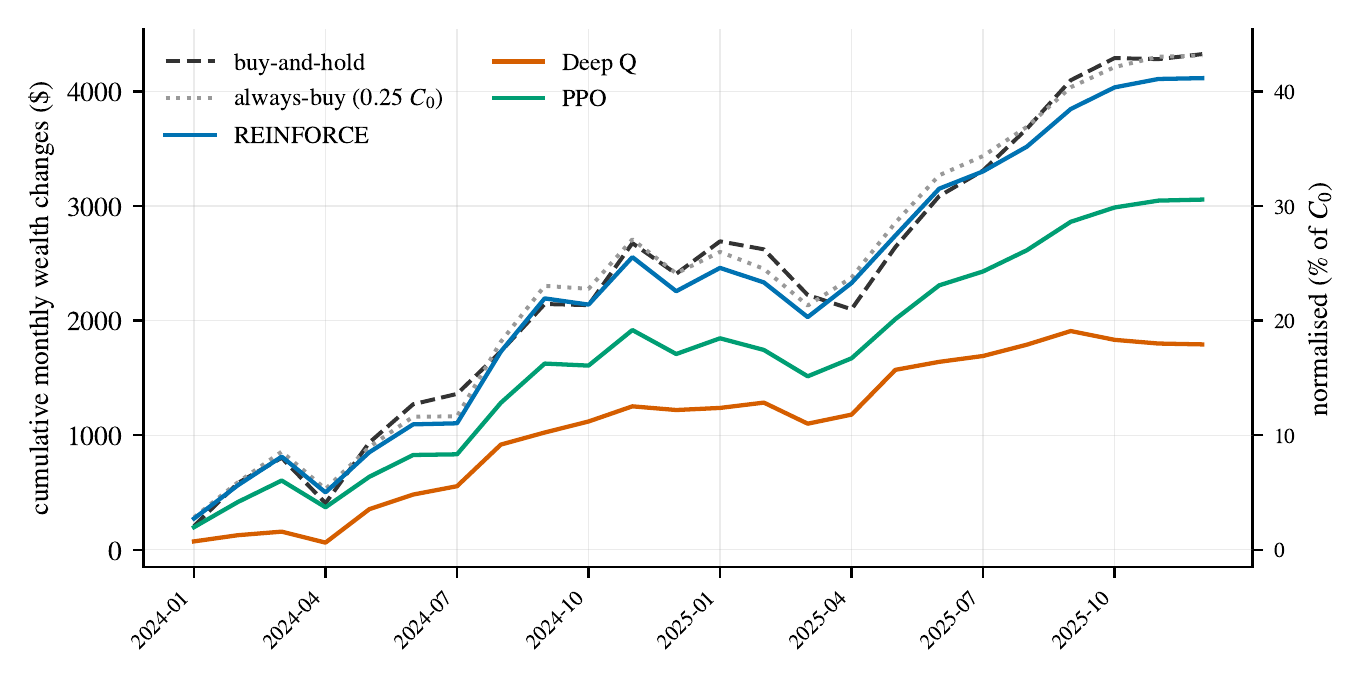
\includegraphics[width=0.9\textwidth]{media4/media/image5.png}
  \caption[Cumulative sum of average monthly wealth changes across the test months.]{Cumulative sum of average monthly wealth changes across the test months. Each monthly episode resets to C₀, so the lines show the sum of monthly gains and losses rather than compound; the right axis expresses percentages of initial capital C₀. REINFORCE follows Always-buy (0.25 C₀) and buy-and-hold almost exactly, while Deep Q-learning shows a flatter line due to low exposure, including through the March--April 2025 decline.}
\end{figure}


Over the full two years, the gap compounds visibly in Figure 5.3:
buy-and-hold accumulates to +\$4,326 in monthly wealth change at the end
of 2025, REINFORCE to +\$4,116 closely following buy-and-hold, PPO to
+\$3,056, and Deep Q-learning at the lowest value of +\$1,792.

\subsection{Return and market exposure}

The exposure column explains most of the return column. The REINFORCE
result is particularly interesting; its return was close to buy-and-hold
at +\$171.51. Its average exposure was 0.810, compared with 0.913 for
buy-and-hold, and none of its six seeds were state-dependent, suggesting
the high return came mainly from staying invested rather than learning
when to enter or leave the market. Its behaviour was therefore closer to
the Always-buy at \(0.25C\) accumulation strategy. Hence why it sits
within a few percent of Always-buy results (+\$179.75, exposure 0.841).

DQN produced a different result. All six seeds were state-dependent,
showing that the agent changed its actions in response to state
information, and chose to participate the least, with the lowest
exposure of 0.312 and a wealth change of \$74.68. These results are
roughly a third of the buy-and-hold benchmarks, so the lower return may
therefore be correlated with reduced market participation.

PPO produced a return between REINFORCE and DQN, with an average wealth
change of \$127.35 and exposure of 0.598. However, its seed spread was
179.8, which is larger than its mean return. This shows that the six PPO
runs produced different outcomes and should not be treated as a single
stable trading strategy.

\subsection{Risk and risk-adjusted performance}

Lower returns can still be desirable if they follow a sufficient
reduction in risk. For this reason, drawdown and Sharpe ratio are also
used alongside return. Figure 5.4 puts every learned configuration in
this chapter on that scale.

\begin{figure}[!htb]
  \centering
  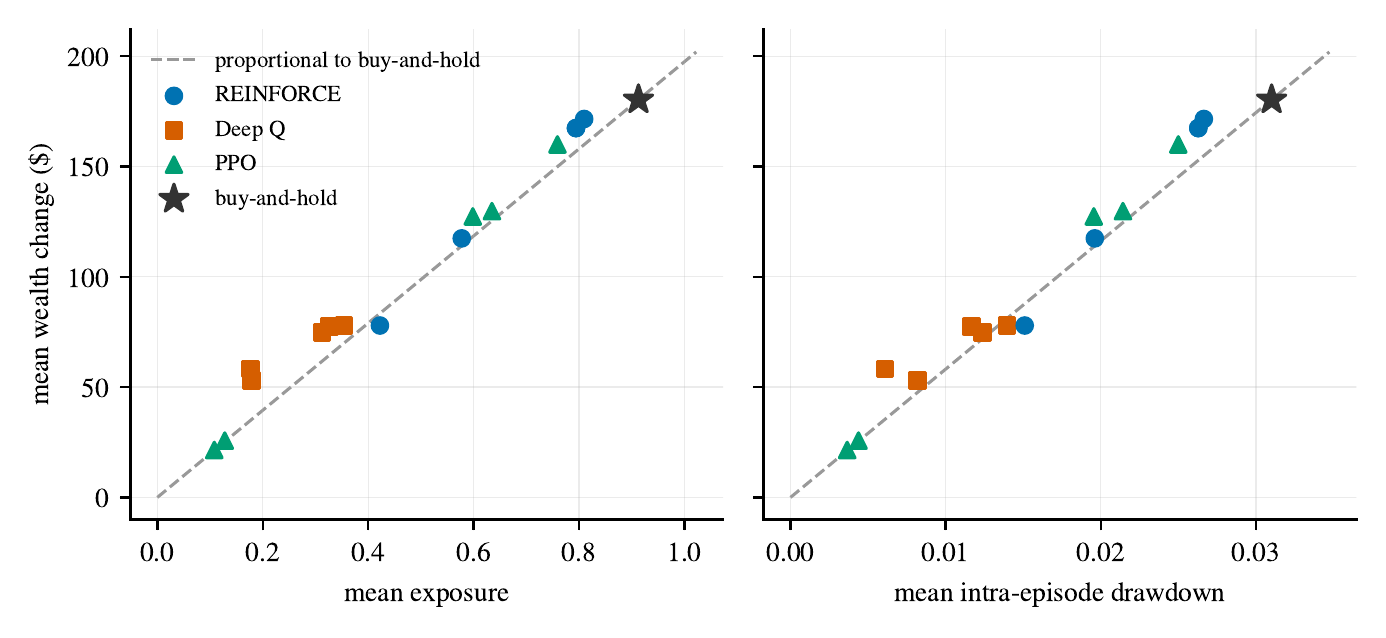
\includegraphics[width=0.9\textwidth]{media4/media/image6.png}
  \caption[Average wealth change compared with exposure (left) and daily drawdown (right) for every learned configuration in this chapter.]{Average wealth change compared with exposure (left) and daily drawdown (right) for every learned configuration in this chapter. The dashed lines show the proportional relationship with buy-and-hold. None of the learned configurations show a clear improvement over either line.}
\end{figure}


Buy-and-hold earned \$197 per unit of exposure. An agent that merely
holds less of the same asset lands on the dashed proportional line;
genuine downside management would appear above it.

Deep Q-learning is an informative case. It earned 41.4\% of the
buy-and-hold benchmark's return at 34.2\% of its exposure (0.312) and
40.0\% of its drawdown (0.0124) --- return and risk fell equally, which
is more like scaling down. Its Sharpe ratio of 0.507 versus
buy-and-hold's 0.638 confirms it earned less return per unit of risk
exposed to, not more.

The results therefore do not indicate that DQN achieved better
risk-adjusted performance than the benchmark. Its lower drawdown largely
came from lower exposure, not from a strategy that intentionally avoided
the market\textquotesingle s decline periods.

\subsection{Behaviour During the March 2025 Decline}

March 2025 provides a useful example because it was the worst test month
for the buy-and-hold benchmark. During this month, buy-and-hold lost
\$398.41, i.e. 3.9841\% of the initial capital, with a drawdown of
approximately 5.6\%. If the state-dependent agent, Deep Q-learning, had
recognised the conditions, this would have been the month to step aside.
Instead, DQN had a mean exposure of 0.490 in March--- higher than its
overall average exposure of 0.312 for the entire test period--- and lost
\$184.04, 46\% of the benchmark's loss.

These results are important when interpreting the state-dependence
finding. Even in a month when reducing exposure before the decline could
have helped, it did not significantly reduce exposure, and these March
2025 losses match its equivalent market participation. Hence, its lower
drawdown cannot be attributed to knowing when to avoid bad market
periods, but to holding less overall.

\begin{figure}[!htb]
  \centering
  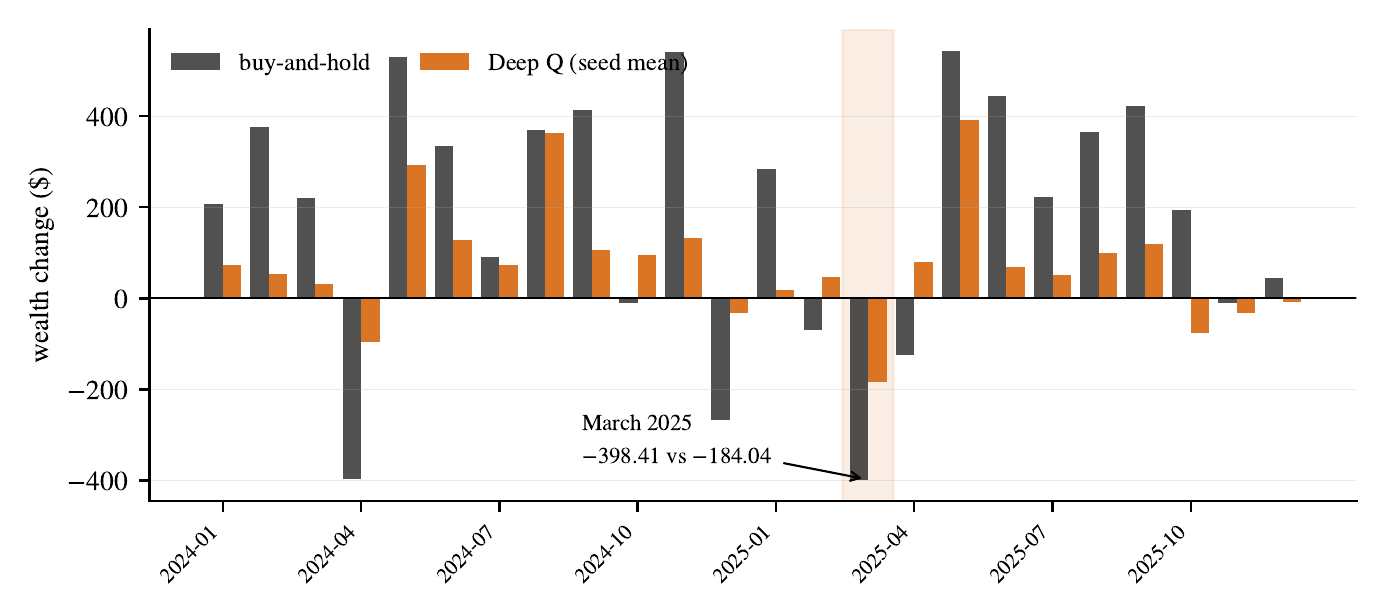
\includegraphics[width=0.9\textwidth]{media4/media/image7.png}
  \caption[Monthly wealth changes of buy-and-hold and Deep Q-learning over the 24 test months.]{Monthly wealth changes of buy-and-hold and Deep Q-learning over the 24 test months. The agent's bars match a 1/3 scaling of the benchmark's bars in almost every month: In March 2025, the worst month, it lost \$184.04 compared to the benchmark's \$398.41 loss.}
\end{figure}


Figure 5.5 extends to all 24 months. Each pair of bars is one test
month: the dark bar represents buy-and-hold's wealth change, and the
orange bar represents the Deep Q-learning for the same month. The two
series appear to rise and fall together --- the agent's best month is
the benchmark's best month (May 2025, +\$390.80 compared to +\$543.11)
and its worst is the benchmark's worst (the discussed March 2025).

Buy-and-hold lost money in seven of the 24 months, and the agent ended
positive in three of those seven. Those three months, however, produced
little profit compared to the benchmark losses

In the two heavy down months, April 2024 (−\$396.08) and March 2025
(−\$398.41), the agent was also at a loss---approximately 24\% and 46\%
of the benchmark's loss, respectively---correlating to its 34\% average
market participation and one-third scaling to the benchmark. Where
drawdown management mattered most, the agent still left the position
open to losses.

\subsection{Trading behaviour and Seed consistency}

The results also show considerable differences in consistency between
the algorithms. To examine this, we analyse seed spreads, which measure
differences between runs.

REINFORCE had the smallest seed spread (\$24.70), showing seeds agree
with each other. However, this consistency should be interpreted with
its behavioural results. All six seeds were classified as
state-independent and exhibited similar behaviour, precisely because
they agree on ignoring market information and generally being highly
exposed, as that is more rewarding. The small spread therefore does not
necessarily indicate that REINFORCE learned a more reliable trading
strategy.

DQN had a larger spread of \$71.40. This is consistent with the six
seeds learning different state-dependent policies, resulting in greater
variations in their returns.

PPO had the largest spread of \$179.80, which was greater than the mean
return, also showing that individual seeds ranged from near-inactivity
to near-full investment in Fig. 5.2, and none were state-dependent.

These results show why evaluating a single random seed would not provide
enough evidence for a reliable conclusion about the learning algorithms.
Behaviour and performance can vary considerably from one training run to
the next.

\section{Effect of the Risk-Aware Reward}

Earlier experiments showed that the main wealth-change reward did not
always encourage agents to respond differently to changes in the
observed state. It simply rewards changes in portfolio wealth.

Chapter 3.5 identifies the limitation of this objective: it does not
penalize large portfolio drawdowns, raising the question of whether
explicitly including portfolio drawdown in the reward would lead to more
risk-aware behaviour.

To examine this, the risk-aware reward was introduced in which it was
modified to include a penalty for increases in drawdown:

\[r_{t}^{risk} = \Delta W_{t} - \lambda C_{0}\Delta dd_{t}.\]

where

\(\Delta dd_{t}\) is the increase in portfolio drawdown at trading day
\(t\) (and is zero when drawdown does not rise), and coefficient
\(\lambda\) controls the penalty effects. The initial capital \(C_{0}\)
factor puts \(\Delta dd_{t}\) in dollars so that 𝜆 is dimensionless.

The risk-aware reward is paired with the ten-feature state using the
drawdown feature because it provides the agent with information about
its current position relative to its previous maximum wealth.

\subsection{Selection of the Penalty size}

The penalty size was selected using the validation set and Deep
Q-learning as the selector because it is the only algorithm whose
policies consistently respond to the state (Section 5.4). The held-out
test period was not used for this decision.

A selection rule was created. The penalised configuration must keep at
least half (50\%) of both the unpenalised return---to still earn a
decent amount --- and the unpenalised exposure---to still participate in
the market.

The unpenalised DQN configuration had a mean wealth change of \$78.35
and exposure of 0.445. The resulting minimum requirements were
therefore:

\[\Delta W \geq \$ 39.17\]

and

\[Exposure \geq 0.223.\]

The results of the penalty sweep are shown in Table 5.5.

{\def\LTcaptype{none} % do not increment counter
\begin{longtable}[]{@{}
  >{\raggedright\arraybackslash}p{(\linewidth - 10\tabcolsep) * \real{0.1900}}
  >{\centering\arraybackslash}p{(\linewidth - 10\tabcolsep) * \real{0.1610}}
  >{\centering\arraybackslash}p{(\linewidth - 10\tabcolsep) * \real{0.1633}}
  >{\centering\arraybackslash}p{(\linewidth - 10\tabcolsep) * \real{0.1652}}
  >{\centering\arraybackslash}p{(\linewidth - 10\tabcolsep) * \real{0.1605}}
  >{\centering\arraybackslash}p{(\linewidth - 10\tabcolsep) * \real{0.1600}}@{}}
\toprule\noalign{}
\begin{minipage}[b]{\linewidth}\centering
\textbf{λ}
\end{minipage} & \begin{minipage}[b]{\linewidth}\centering
\textbf{Mean ΔW}
\end{minipage} & \begin{minipage}[b]{\linewidth}\centering
\textbf{Exposure}
\end{minipage} & \begin{minipage}[b]{\linewidth}\centering
\textbf{Drawdown}
\end{minipage} & \begin{minipage}[b]{\linewidth}\centering
\textbf{DD change}
\end{minipage} & \begin{minipage}[b]{\linewidth}\centering
\textbf{Passes}
\end{minipage} \\
\midrule\noalign{}
\endhead
\bottomrule\noalign{}
\endlastfoot
\textbf{0 (unpenalised)} & +\$78.35 & 0.445 & 0.0163 & --- & --- \\
\rowsep
\textbf{0.05} & +\$88.78 & 0.401 & 0.0128 & −21.5\% & yes \\
\rowsep
\textbf{0.10} & +\$67.30 & 0.344 & 0.0124 & −24.0\% & yes \\
\rowsep
\textbf{0.25} & +\$19.90 & 0.074 & 0.0035 & −78.4\% & no \\
\rowsep
\textbf{0.50} & +\$1.73 & 0.002 & 0.0001 & −99.4\% & no \\
\rowsep
\textbf{1.00} & \$0.00 & 0.000 & 0.0000 & −100\% & no \\
\rowsep
\textbf{2.00} & \$0.00 & 0.000 & 0.0000 & −100\% & no \\
\end{longtable}
}

\addcontentsline{lot}{table}{\protect\numberline{5.5}{Risk-penalty size on the validation months (Deep Q-learning, six seeds). The rule requires ΔW ≥ +\$39.17 and exposure ≥ 0.223; the largest passing value that meets both requirements is λ = 0.10.}}
\emph{Table 5.5: Risk-penalty size on the validation months (Deep
Q-learning, six seeds). The rule requires ΔW ≥ +\$39.17 and exposure ≥
0.223; the largest passing value that meets both requirements is λ =
0.10.}

\begin{figure}[!htb]
  \centering
  
\includegraphics[width=0.9\textwidth]{media5/media/image1.png}
  \caption[Results from the penalty size of Table 5.5. Left: mean wealth change against λ with the requirement floor of +\$39.17. Right: exposure and drawdown relative to their values without penalties.]{Results from the penalty size of Table 5.5. Left: mean wealth change against λ with the requirement floor of +\$39.17. Right: exposure and drawdown relative to their values without penalties. Between λ = 0.10 and 0.25, exposure drops sharply rather than decreasing gradually.}
\end{figure}


The results show a clear change in behaviour of the penalty \(\lambda\)
as the size increases. At \(\lambda = 0.10\) , the agent still maintains
a meaningful level of exposure and a return of \$67.30.

Increasing the penalty to 0.25 causes exposure to fall sharply to 0.074.
The agent loses about 78\% of its exposure, indicating reluctance to
trade. At \(\lambda = 0.50\) and above, the agent stops trading
completely.

This result depicts an important limitation of the reward formulation.
The simplest way for an agent to reduce drawdown is to hold less of the
asset or simply not hold it at all. In theory, a portfolio that remains
in cash is not exposed to asset movements and therefore does not
experience market drawdowns. Once the drawdown penalty becomes too
large, market participation becomes unattractive.

Based on these criteria, the largest coefficient that satisfied both the
return and exposure requirements was therefore:

\[\boxed{\lambda = 0.10}.
\]This became the fixed penalty value for evaluating the main risk-aware
experiment.

\subsection{Effect on the Test Set}

The selected risk-aware reward was then evaluated on the held-out test
set.

{\def\LTcaptype{none} % do not increment counter
\begin{longtable}[]{@{}
  >{\raggedright\arraybackslash}p{(\linewidth - 14\tabcolsep) * \real{0.1675}}
  >{\centering\arraybackslash}p{(\linewidth - 14\tabcolsep) * \real{0.1192}}
  >{\centering\arraybackslash}p{(\linewidth - 14\tabcolsep) * \real{0.1202}}
  >{\centering\arraybackslash}p{(\linewidth - 14\tabcolsep) * \real{0.1162}}
  >{\centering\arraybackslash}p{(\linewidth - 14\tabcolsep) * \real{0.1364}}
  >{\centering\arraybackslash}p{(\linewidth - 14\tabcolsep) * \real{0.1125}}
  >{\centering\arraybackslash}p{(\linewidth - 14\tabcolsep) * \real{0.1117}}
  >{\centering\arraybackslash}p{(\linewidth - 14\tabcolsep) * \real{0.1162}}@{}}
\toprule\noalign{}
\begin{minipage}[b]{\linewidth}\centering
\textbf{Algorithm}
\end{minipage} & \begin{minipage}[b]{\linewidth}\centering
\textbf{Reward}
\end{minipage} & \begin{minipage}[b]{\linewidth}\centering
\textbf{ΔW (\$)}
\end{minipage} & \begin{minipage}[b]{\linewidth}\centering
\textbf{Spread}
\end{minipage} & \begin{minipage}[b]{\linewidth}\centering
\textbf{Exposure}
\end{minipage} & \begin{minipage}[b]{\linewidth}\centering
\textbf{Trades}
\end{minipage} & \begin{minipage}[b]{\linewidth}\centering
\textbf{DD}
\end{minipage} & \begin{minipage}[b]{\linewidth}\centering
\textbf{Sharpe}
\end{minipage} \\
\midrule\noalign{}
\endhead
\bottomrule\noalign{}
\endlastfoot
\textbf{REINFORCE} & wealth & +167.39 & 24.7 & 0.794 & 13.0 & 0.0263 &
0.670 \\
\rowsep
\textbf{REINFORCE} & risk & +167.39 & 24.7 & 0.794 & 13.0 & 0.0263 &
0.670 \\
\rowsep
\textbf{Deep Q} & wealth & +77.81 & 89.5 & 0.354 & 7.4 & 0.0140 &
0.505 \\
\rowsep
\textbf{Deep Q} & risk & +52.90 & 43.1 & 0.178 & 5.4 & 0.0082 & 0.416 \\
\rowsep
\textbf{PPO} & wealth & +159.97 & 94.0 & 0.759 & 7.3 & 0.0250 & 0.671 \\
\rowsep
\textbf{PPO} & risk & +21.48 & 128.9 & 0.108 & 0.7 & 0.0037 & 0.107 \\
\end{longtable}
}

\addcontentsline{lot}{table}{\protect\numberline{5.6}{Wealth-change versus risk-aware reward (λ = 0.10) on the held-out months, ten-feature state, six seeds.}}
\emph{Table 5.6: Wealth-change versus risk-aware reward (λ = 0.10) on
the held-out months, ten-feature state, six seeds.}

The DQN result gives the clearest evidence of the effect of the
risk-aware reward. For Deep Q-learning, the mean drawdown falls from
0.0140 under the standard reward to 0.0082 with the risk-aware reward, a
reduction of approximately 41\%. However, its return also falls from
+\$77.81 to +\$52.90, a reduction of about 32\%. Exposure falls from
0.354 to 0.178, meaning that the agent decides to hold only half as much
of the asset.

The results do not suggest improved risk-adjusted performance. Instead,
the reward mainly encouraged the agent to reduce its exposure to the
asset, and the Sharpe ratio also decreased from 0.505 to 0.416.

The PPO results show the same effect more strongly. With the risk-aware
reward, PPO\textquotesingle s exposure fell to 0.108, and its average
trading activity dropped below one trade per month, from 7.3 to 0.7. As
a result, its mean wealth change decreased from \$159.97 to +\$21.48.

REINFORCE shows no noticeable change. Its results are identical for both
rewards. This is consistent with the earlier behavioural findings:
REINFORCE policies do not change their trading behaviour simply by
changing the reward.

\subsection{Interpretation of the risk-aware return}

The risk-aware reward changed the behaviour of the state-dependent
agents, but there is no clear evidence that it led to better risk
management. Instead, the results suggest that the penalty mainly
encouraged the agents to reduce their exposure to the asset.

These results do not show that risk-aware reinforcement learning is
ineffective in general. However, they do show a limitation of the reward
formulation used in this study. An agent's policy could reduce drawdown
to zero by simply holding less of that asset or by never entering the
market, but this would not satisfy the main objective of generating
useful investment returns.

A more effective objective would therefore need to consider both return
and risk, rather than mainly penalising exposure to drawdown. The
relevant question becomes whether the agent can \textbf{reduce drawdown
while still leading to meaningful returns and exposure.} For example,
the objective could reward the agent for achieving higher returns for a
given level of risk. Chapter 6 discusses other possible alternatives in
future work.

\section{Transaction-Fee Sizing}

Transaction costs are an important part of the trading environment
because frequent trading can reduce the returns produced by a strategy,
even when individual decisions appear reasonable. A strategy may appear
profitable before fees are included but become less attractive once the
cost of each trade is taken into account.

The main experiments use a transaction fee of 0.05\%. To test whether
the observed behaviour changes as this fee varies, the fee was swept
from 0 basis points (0.00\%) to 50basis points (0.50\%) on the
validation months with the nine-feature state, and everything else held
fixed.

The sweep was run on all algorithms, each with six freshly trained seeds
per fee level. Table 5.7 and Figure 5.7 report the outcome.

{\def\LTcaptype{none} % do not increment counter
\begin{longtable}[]{@{}
  >{\raggedright\arraybackslash}p{(\linewidth - 14\tabcolsep) * \real{0.1320}}
  >{\centering\arraybackslash}p{(\linewidth - 14\tabcolsep) * \real{0.1243}}
  >{\centering\arraybackslash}p{(\linewidth - 14\tabcolsep) * \real{0.1242}}
  >{\centering\arraybackslash}p{(\linewidth - 14\tabcolsep) * \real{0.1237}}
  >{\centering\arraybackslash}p{(\linewidth - 14\tabcolsep) * \real{0.1242}}
  >{\centering\arraybackslash}p{(\linewidth - 14\tabcolsep) * \real{0.1237}}
  >{\centering\arraybackslash}p{(\linewidth - 14\tabcolsep) * \real{0.1242}}
  >{\centering\arraybackslash}p{(\linewidth - 14\tabcolsep) * \real{0.1237}}@{}}
\toprule\noalign{}
\begin{minipage}[b]{\linewidth}\centering
\textbf{Fee}
\end{minipage} & \begin{minipage}[b]{\linewidth}\centering
\textbf{B\&H ΔW}
\end{minipage} & \begin{minipage}[b]{\linewidth}\centering
\textbf{REINF. ΔW}
\end{minipage} & \begin{minipage}[b]{\linewidth}\centering
\textbf{REINF. trades}
\end{minipage} & \begin{minipage}[b]{\linewidth}\centering
\textbf{Deep Q ΔW}
\end{minipage} & \begin{minipage}[b]{\linewidth}\centering
\textbf{Deep Q trades}
\end{minipage} & \begin{minipage}[b]{\linewidth}\centering
\textbf{PPO ΔW}
\end{minipage} & \begin{minipage}[b]{\linewidth}\centering
\textbf{PPO trades}
\end{minipage} \\
\midrule\noalign{}
\endhead
\bottomrule\noalign{}
\endlastfoot
\textbf{0bps(0.00\%)} & +\$177.09 & +\$177.56 & 5.0 & +\$108.00 & 10.9 &
+\$155.35 & 4.5 \\
\rowsep
\textbf{5bps(0.05\%)} & +\$166.92 & +\$154.96 & 10.3 & +\$86.16 & 8.5 &
+\$118.55 & 3.7 \\
\rowsep
\textbf{10bps(0.10\%)} & +\$156.76 & +\$143.74 & 4.7 & +\$77.60 & 8.9 &
+\$78.50 & 2.7 \\
\rowsep
\textbf{25bps(0.25\%)} & +\$126.33 & +\$88.76 & 10.3 & +\$32.35 & 3.9 &
+\$26.40 & 1.2 \\
\rowsep
\textbf{50bps(0.50\%)} & +\$75.83 & +\$41.31 & 2.8 & +\$16.32 & 1.9 &
+\$12.60 & 1.0 \\
\end{longtable}
}

\addcontentsline{lot}{table}{\protect\numberline{5.7}{Transaction Fee sizing on the validation months; six seeds. Trades are per month. Fees are shown in basis points and as a percentage of trade value.}}
\emph{Table 5.7: Transaction Fee sizing on the validation months; six
seeds. Trades are per month. Fees are shown in basis points and as a
percentage of trade value.}

\begin{figure}[!htb]
  \centering
  
\includegraphics[width=0.9\textwidth]{media5/media/image2.png}
  \caption{Transaction Fee sizing from Table 5.7. Left: average wealth change falls for every strategy as fees rise. Right: average trades per month as fees rise.}
\end{figure}


\subsection{Effect of transaction costs on returns \& trading behaviour}

As expected, higher transaction fees reduce the returns of the different
algorithm strategies. The effect is important for strategies that trade
frequently because more of their portfolio gains go to transaction
costs.

Deep Q-learning shows the clearest reduction in trading activity as the
fee of taking a trade increases. Its average number of trades falls from
10.9 per month at 0bps (0.00\%) to 1.9 at 50bps (0.50\%), an 83\%
reduction. As each action gets more expensive, the agent acts less,
reducing exposure. This is consistent with the algorithm correctly
incorporating transaction costs into its environment.

REINFORCE does not show the same clear pattern. Its trade counts vary,
running from 5.0, 10.3, 4.7, 10.3, and 2.8, respectively, with no
consistent decrease in trades taken as the fee rises. This aligns with
the earlier state-independent results: an agent that does not rely on
information from its current state to make decisions is less likely to
adjust its behaviour when trading costs change.

PPO's average trade count also falls from 4.5 to 1.0, showing that many
seeds are pushed to stop trading due to higher fees. This is also why
the average return collapses by 77\%, from +\$177.56 to +\$41.31, a
difference of \$136.25 per month, even though the average trade count
moves only gently.

\subsection{Interpretation}

The transaction-fee experiment therefore reflects another difference
between the learning algorithms in terms of their change in behaviour.
Deep Q-learning changes its trading behaviour as trading costs increase,
even though its overall returns are below the buy-and-hold benchmark. This mirrors the fee response reported by Th\'eate and Ernst, whose agent also traded less as the assumed costs rose~\cite{theate2021}.
REINFORCE produces returns generally closer to the buy-and-hold
strategy, and it also shows higher exposure that does not respond
consistently to changes in transaction costs. PPO, on the other hand,
shows a major collapse in returns as fees increase, while its trade
counts decline more gently. Overall, the learned agents lose
proportionally more because they trade more often in this experiment.

This indicates that the learning system is capable of responding to
different changes when the learned policy is sufficiently
state-dependent.

\section{Discussion of the Main Findings}

The experiments produced several findings about both the performance of
the learning agents and the way they behaved within the trading
environment. They also answer the research questions of Section 5.1

\subsection{The Benchmark Remains Difficult to Beat}

The main finding is that none of the learned agents could outperform the
simple buy-and-hold benchmark on the held-out test period. Buy-and-hold
achieved a wealth change of \$180.25, compared with \$171.51 for
REINFORCE as the best learned agent, while every other agent fell
further behind with \$127.35 for PPO, and \$74.68 for DQN.

However, it is important to note that the test period consists of
generally favourable market conditions. Therefore, the experiments
cannot simply be viewed as evidence that reinforcement learning failed,
as staying invested in generally rising markets is already a strong
strategy

Buy-and-hold is therefore a difficult benchmark to improve upon, which is consistent with the market-efficiency expectation set out in Chapter 2~\cite{fama1970}. A
learned strategy that reduces exposure must therefore focus on periods
when leaving the market is advantageous enough to compensate for the
return not gained while being out of the market.

The experiments provide limited evidence that the tested agents could
make this decision and overall did not demonstrate such behaviour.

\subsection{Additional State Features Did Not Lead to Better Performance}

The state comparison did not show a consistent advantage from adding
drawdown to the nine-feature state. This is important because the state
representation was designed to include information about market
movements, portfolio position, wealth, and risk.

For REINFORCE and DQN, the changes in return were -\$4.12 and \$3.13,
respectively, in the nine-to-ten-feature comparison. This does not
necessarily mean the features were poorly selected, nor that the
nine-feature state is universally sufficient. It means that, in this
particular environment and with this wealth-change objective, additional
market information produced no measurable improvement. The later
risk-aware experiments show the behaviour changing only when the
objective itself included drawdown, and mainly through reduced market
participation.

\subsection{The Algorithms Differed in Their Use of the State}

One of the clearest differences between the algorithms is behavioural
rather than financial. REINFORCE and PPO often produced policies that
were classified as state-independent, so their relatively strong returns
need careful interpretation: a policy that buys whenever possible can
perform well in rising markets without using the information provided to
it. Deep Q-learning was state-dependent in all six seeds, but its use of
the state generally reduced exposure rather than raising returns.

This is why financial return alone is not enough to evaluate the learned
policies. Without the behavioural analysis, the strong performance of
REINFORCE could be mistaken for evidence that the model had learned a
useful relationship between market information and trading decisions.

\subsection{Lower Risk Was Mainly Associated with Lower Exposure}

The results show a consistent relationship between market participation
and risk; specifically, risk was reduced mainly by participating less in
the market.

Deep Q-learning achieved lower drawdown than buy-and-hold, but this was
due to lower exposure, and overall, it led to lower returns in the same
proportion.

This means lower drawdown should not be interpreted as evidence that DQN
avoided the worst market movements, as this differs from identifying and
avoiding specific periods of downside markets.

A proper risk-management strategy would ideally remain invested during
rising market periods while reducing exposure during market downsides
once detected. The current results do not provide enough evidence to
conclude that the agent learned this type of selective risk management.

\subsection{The Trade Size Affects Performance}

The trade size experiment shows that the transaction size is part of the
problem definition rather than merely an implementation design. A small
trading size limits how much exposure an agent can build during a
monthly episode, so poor performance may stem from the trade size rather
than the quality of the learned policy. The calibration in Section 5.3
addressed this by selecting the \(0.25C_{0}\) size, which brings the
attainable exposure close to the benchmark\textquotesingle s. Notably,
changing the trade size had a larger effect on performance than adding
features to the state, which supports calibrating it before working on
the main learned strategies.

\subsection{Transaction Costs Provided a Useful Behavioural Test}

The transaction-fee experiment showed that Deep Q-learning reduced its
trading activity by approximately 83\% as the fee rose from zero to
0.50\%, while REINFORCE did not show the same response. This provides
further evidence that Deep Q-learning was making greater use of the
information available through the environment, although this additional
responsiveness did not result in better financial performance.

\subsection{Variation Between Seeds Is Important}

This experiment showed considerable variation between random seeds,
especially for the policy-gradient methods.

In some configurations, different seeds produced noticeably different
behaviours. Some policies turned towards high exposure, while others
traded less or became more conservative.

A seed producing a strong return would not be enough to conclude that
the algorithm had learned a reliable trading strategy. Consistent
behaviour across multiple seeds proves that, and becomes stronger
evidence that, the observed result is derived from that algorithm rather
than a product of one training run.

\subsection{Implications for the Research Objectives}

Overall, the experiments provide a qualified answer to the main research
question of whether reinforcement learning algorithms can learn
profitable trading strategies for a portfolio (in this case, the SPY
asset).

The reinforcement learning agents learned trading policies, but the
experiments did not show they could outperform the simpler buy-and-hold
benchmark on unseen data.

The results also show that learning behaviour strongly depends on the
algorithm, with clear differences between the learning methods.
REINFORCE moved towards remaining invested and made little use of state
information. DQN, however, consistently changed its actions based on the
observed state, making it highly state-dependent, but it did not yield
higher returns.

PPO behaviour was closer to REINFORCE than to DQN. Although PPO uses an
actor-critic structure and a clipped policy objective to stabilise
updates, its performance was less consistent across seeds, with a larger
spread in returns. This suggests that PPO\textquotesingle s additional
stability mechanisms did not produce an effective trading policy in this
environment.

The risk-aware reward also changed the behaviour of the state-dependent
agents and reduced drawdown, but the reduction was mainly due to lower
market exposure rather than better timing for entering and exiting
markets during downward periods. When the penalty became too large, the
agents almost stopped trading altogether.

These findings suggest that the main challenge identified by the
experiments is not just related to providing the agent with more
information. Instead, the results strongly point to the interaction
between the \textbf{reward function, trade size, and the behaviour
learned by the agent} as key factors in determining whether the
resulting strategy is useful.

\section{Chapter Summary}

The chapter first determines the final trade size because this affects
how quickly an agent can build or reduce its position. It then examines
whether the learned strategies rely on the information from the state
representations, followed by a comparison between the main nine-feature
state and the additional risk-aware state. It then presents the main
held-out test results, followed by experiments on the risk-aware reward
and the effect of transaction costs. The chapter concludes by bringing
the findings together and relating them to the research objectives.

The results show that none of the learned agents consistently
outperforms the buy-and-hold benchmark over the held-out dataset. The
behavioral analysis offers more insight into this outcome. The
policy-gradient algorithms rely less on available state information,
whereas the value-based agent uses more available state information but
generally has a lower exposure. The experiments also indicate that the
fixed trading amount affects performance. Finally, the drawdown-based
reward reduces both return and exposure, suggesting that the risk-aware
reward mainly encourages lower market participation rather than
generating better risk-adjusted trading performance.


\chapter{Conclusion and Future Work}
\section{Summary of the Work}

This dissertation examined whether reinforcement learning algorithms can
learn profitable trading policies that utilize market and portfolio
information from the observed states when trading assets in a portfolio.

The study designed a complete experimental system for trading the SPY
exchange-traded fund. The system uses daily market data organised into
monthly episodes, includes transaction costs and action masking, and
uses a nine-feature state representation with an optional drawdown
feature. Two reward formulations were tested: the primary wealth-change
reward and an optional risk-aware reward that penalised drawdown, along
with three learning algorithms: REINFORCE, Deep Q-learning (DQN), and
Proximal Policy Optimisation (PPO).

Experimental decisions were made on the 12-month validation dataset
(2023), while keeping the 24-month test set (2024-2025) separate and
using it only for final evaluations.

The experiments followed a fixed sequence. First, the trade size was
adjusted to ensure the agents could reach a reasonable level of exposure
relative to the buy-and-hold benchmark. The behavioural experiment then
determined whether the learned policies actually respond to the
information in their states. Once these environment, calibration and
behavioural choices had been decided, the main performance of the
learned agents was evaluated and compared against the benchmark strategy
on the unseen test period.

Additional experiments then tested whether adding drawdown to the state
changed the results, whether a risk-aware reward improved loss
management in the portfolio trade, and how the different learning
methods responded to changes in transaction costs.

\section{Conclusions Against the Research Questions}

The experiments in Chapter 5 address the four questions asked in 5.1.

\subsection{Performance}

The first question considered whether the reinforcement learning agents
could outperform the buy-and-hold benchmark on unseen data.

The results do not provide any evidence that they could. No learned
agent outperformed the simple buy-and-hold strategy on the held-out test
period. Buy-and-hold produced a mean wealth change of +\$180.25 per
month, while the best learned agent, REINFORCE, achieved +\$171.51. PPO
achieved +\$127.35 and DQN +\$74.68.

The result should not be interpreted as reinforcement learning
algorithms being incapable of learning profitable trading strategies.
All agents produced positive average wealth changes. Instead, the more
specific conclusion is that none of the tested algorithms learned a
level of trading skill that could outperform the simple investment
strategy on unseen data.

Transaction costs and the trade size also cannot explain the difference,
since they were the same throughout the experiment, providing a basis
for fair comparison. The test period, however, favoured remaining
invested, with positive market performance in 17 of the 24 months. Under
these conditions, buy-and-hold was difficult to beat as it benefits from
the rising market direction.

\subsection{Behaviour}

The second question examined whether the learned policies genuinely use
the state information provided to them.

The algorithms showed a clear difference in how they used the state. All
six DQN seeds changed their actions in response to the observed state,
while none of the twelve policy-gradient seeds from REINFORCE and PPO
did so. This changes how the performance results should be interpreted.
REINFORCE came close to the benchmark in terms of return, at +\$171.51
per month, but its policies largely shifted to buying rather than using
the market information provided.

DQN however produced policies that consistently responded to changes in
the observed state but produced a lower average return than REINFORCE.
This suggests that state dependence and financial performance are not to
be treated as equal objectives in the experimental setting. An agent can
learn to use its observations without that behaviour necessarily
yielding higher returns.

This differentiation is important because an agent can perform well for
the wrong reason. During a generally rising market, a policy that
remains invested can achieve a strong return without needing to learn
when market conditions require entering, reducing, or exiting a
position.

Looking only at return would have completely hidden the distinction
between these behaviours. The behavioural analysis is therefore an
important part of evaluating learned trading policies, as it revealed a
clear difference between the value-based and policy-gradient methods.

\subsection{State Representation}

The third question examined whether adding a drawdown feature to the
state representation improved agent performance or behaviour.

Adding drawdown to the nine-feature state produced only limited changes
using the wealth-change reward. REINFORCE\textquotesingle s mean monthly
wealth change decreased by \$4.12, while DQN\textquotesingle s increased
by \$3.13. Both changes were small compared with the variation between
their random seeds and cannot be reasonably treated as reliable
improvements.

PPO\textquotesingle s mean return increased by \$32.62, but its seed
spread also changed heavily, from \$179.80 to \$94.00. This improvement
cannot confidently be attributed to the drawdown feature itself.

Overall, the results suggest that providing additional information does
not automatically produce a better policy or improve learning unless the
objective specifies it. This is consistent with an important principle
noticed from the experiments: \textbf{information in the state is only
useful when the learning objective and optimisation process give the
agent a reason to use it}. Hence, the agent must be able to learn a
relationship between the additional information and actions that improve
the objective being optimised.

\subsection{Reward Formulation}

The fourth question considered whether adding drawdown into the reward
could encourage the agents to reduce losses and generate a more
risk-aware behaviour.

The risk-aware reward reduced drawdown mainly by reducing market
participation, not by improving understanding of market conditions. With
the selected penalty of \(\symbf{\lambda = 0.10}\),
DQN\textquotesingle s mean drawdown fell by 41\%, from 0.0140 to 0.0082.
However, its mean return also fell by 32\%, from +\$77.81 to +\$52.90,
while its exposure was approximately halved. Its Sharpe ratio fell from
0.505 to 0.416, so the reduced drawdown did not result in better
risk-adjusted performance. The reward therefore encouraged the agent to
hold less of the asset rather than to identify and avoid declining
markets. This is also reflected in March 2025, when reducing exposure
would have been particularly useful: DQN\textquotesingle s exposure
during the month was higher than its overall average, and it still
experienced 46\% of the benchmark\textquotesingle s loss.

The result illustrates an important limitation of using drawdown as a
standalone penalty. The easiest way for an agent to reduce exposure to
drawdown is to reduce its participation in the market. This behaviour
can theoretically satisfy the risk conditions of the reward without
necessarily producing a better ability to identify when the market is
likely to decline.

The penalty-weight analysis proves this interpretation. A relatively
small increase in the penalty produced a major behavioural change, with
exposure falling from 0.344 at λ = 0.10 to 0.074 at λ = 0.25. This
indicates that the reward formulation created a strong correlation
between market participation and risk avoidance.

\section{Critical Appraisal of the Project}

The most important lessons from this project were from the experimental
methodology rather than the choice of reinforcement learning algorithm
alone. Several of the most useful findings came from implementation
problems identified during development and testing.

One of the strongest aspects of the project was the verification tests.
The automated tests identified several implementation problems during
development, \textbf{three of which could have affected the
experiments' validity}. These
included issues with rolling feature calculation at the end of monthly
episodes and an implementation error in the buy-and-hold benchmark that
reduced its performance by \$38.95 per month, about 21.6\%. If this
error had remained, the dissertation\textquotesingle s main conclusion
could have been misleading, as the learned agents would have appeared to
outperform the benchmark.

The verification tests also noticed the experimental design problem in
the trade size. Using the original \(0.10C_{0}\) trade size in Chapter 3
would make the maximum attainable exposure only 0.690, compared with
0.910 for buy-and-hold. This meant that the learning agents were at a
disadvantage before training even began. Selecting \(0.25C_{0}\) allowed
a fairer comparison while still letting the agents control their
positions in smaller steps than the\(0.50C_{0}\) alternative.

The complete set of 21 verification tests passed before the final
experiments were accepted, giving a higher confidence that the reported
results reflect an appropriate experimental design rather than
implementation errors.

The behavioural analysis was another important part of the study.
Without it, the REINFORCE result of +\$171.51 could have been
interpreted as evidence that the agent had learned an intelligent,
effective trading strategy. The analysis showed this interpretation was
not justified, as the policies acted like a consistent buyer because the
market was consistently rising, completely changing the interpretation
of the result.

The project also highlighted the importance of random seed variation.
The results, particularly for PPO, varied considerably between
independent training runs. PPO had a seed spread of \$179.80 in one
configuration, which was greater than its mean return. This made it
difficult to draw conclusions based on individual training runs, as that
would have been unreliable. Reporting multiple seeds widened the
evaluation, providing a more consistent view of how each algorithm
behaved, although it increased the computational and experimental
workload; however, six seeds are still lacking for more definite
statistical inference.

Overall, the project demonstrated that careful experimental design is as
important as the choice of reinforcement learning algorithm. The main
lessons came from testing the assumptions behind the experiments, rather
than from simply comparing model returns. State dependence, action
constraints, reward design, and seed variation all affect how the final
results could be interpreted. This made the experimental process more
demanding but also produced a more reliable basis for evaluating the
learned trading policies.

\section{Limitations}

The findings of this study should be considered within the scope of the
experimental design, but there are several limitations.

\subsection{One asset and a limited market period}

The experiments use SPY as the only asset, and the held-out period from
2024 to 2025 was generally favourable to holding the asset due to rising
markets. A market with a longer or more severe decline could produce
different results for the learned agents and the buy-and-hold benchmark.
The findings cannot therefore be automatically generalised to other
assets or market conditions without further testing.

\subsection{Monthly Episode Structure}

The trading environment treated each calendar month as a separate
episode. Every episode started with the same initial capital of
\$10,000, and any remaining position was closed at the end of the month.
As a result, the results do not represent a single portfolio that
continuously compounds over the full evaluation period as a real
portfolio would.

This design made the experiments easier to control by keeping the
episode length and starting conditions consistent. However, it also
means that gains or losses from one month did not affect the starting
capital or portfolio position in the following month, which does not
represent a real-world portfolio. A longer continuous portfolio
environment could therefore lead to a different behaviour, especially
for policies that require accumulated wealth or changes in portfolio
value over time.

\subsection{Fixed Trade Size}

The agents trade fixed fractions of the initial capital rather than
choosing their position size continuously. This was calibrated to create
a controlled, reasonable environment for comparison with the benchmark,
but it restricts how much the agents can express their decisions. A
continuous position-sizing model could potentially respond differently
based on its exposure in a particular market condition. Rather than
repeatedly applying fixed buy or sell actions, such an agent could
select its desired portfolio exposure, producing different results in
returns and trading behaviour.

\subsection{Limited Number of Seeds and Lack of Significance Testing}

Six seeds were used for each configuration, and the seed-level results
and variation between them are reported throughout the results. This is
stronger than relying on a single training run, but it does not provide
sufficient statistics for formal claims about small differences. For
example, the \$3.13 change observed for DQN and \textbf{−\$4.12} for
REINFORCE when the state representation was changed is not large enough
to be treated as a meaningful improvement.

\subsection{Risk Penalty Selection was based on DQN}

The reward\textquotesingle s penalty weight λ was selected using DQN
because it was the algorithm that consistently showed state-dependent
behaviour. This does not guarantee that the same penalty value is
appropriate for REINFORCE or PPO, as it was not independently optimised
for every algorithm. A separate calibration for each algorithm could
produce different results. This limitation is particularly relevant
because the algorithms responded differently to the state and reward
formulation.

\subsection{The risk penalty only targets drawdown}

The risk-aware reward penalises drawdown but does not directly measure
whether the return achieved is sufficient for the level of risk taken.
While drawdown is directly relevant to losses, it does not fully
represent the portfolio risk. A reward that relates return to risk,
rather than penalizing risk alone, was not tested.

Additionally, as shown in Section 5.7, the agents could reduce the
penalty simply by reducing their exposure to the asset or not trading at
all. The experiments showed that a lower drawdown value should not
automatically be associated with evidence of better risk management.

\section{Future Work}

The limitations above suggest several directions for furthering the
research. Each stems directly from a limitation or an unresolved result
in the experiments. The behavioural analysis should also be applied to
these future works to determine the agent's behaviour to changes
alongside performance improvements.

\subsection{Longer and More Challenging Market Periods}

The experiments could be repeated over longer market periods containing
more market declines. A useful change would be to use a walk-forward
training approach, allowing the agents to be retrained as market
conditions change. The current study provides useful evidence for a
generally rising test period, but testing market declines would provide
a balanced evaluation of the portfolio.

This would better reflect the changing nature of financial markets,
allowing the system to encounter different combinations of rising,
falling, and volatile conditions. Such an evaluation would also better
test the agents' risk-aware behaviour during downtrends.

\subsection{Predictive and Uncertainty-Aware State Information}

The drawdown feature describes the portfolio\textquotesingle s previous
losses but does not provide information about future market movements.
Future work could therefore include predictive information, such as
probabilistic forecasts containing estimates of forecast uncertainty.

This would give a state-dependent agent more useful information for
making decisions about future market conditions rather than relying only
on historical data. It would also directly test whether
DQN\textquotesingle s ability to use the state leads to more useful
market understanding and trading decisions.

\subsection{Risk-Efficiency Objectives}

The most direct correction to the drawdown penalty could be to replace
it with a reward that considers return relative to risk, such as a
Sharpe-based or drawdown-relative objective~\cite{moody2001}. This would make simply
reducing market exposure a less effective way of improving the reward,
as seen in the current experiments.

The results in Section 5.7 make this future rework highly relevant
because the tested penalty mainly caused agents to reduce exposure
rather than learn when downside risk is increasing.

\subsection{More Seeds for Better Statistical Analysis}

More random training seeds would improve the reliability of comparisons~\cite{henderson2018}
between algorithms and configurations\textbf{.} Future work should
combine this with appropriate statistical analysis to determine whether
observed differences between configurations are likely to represent
genuine results rather than random noise.

\subsection{More flexible trade sizes}

Future experiments could allow the agent to choose its position size
continuously rather than using fixed trade amounts. This would remove
the exposure limit created by the current environment and allow the
agent to express different levels of confidence by adjusting its
position size, potentially enabling smoother portfolio adjustments.

\section{Closing Remarks}

This dissertation examined whether standard reinforcement learning could
beat the simple buy-and-hold strategy on unseen data. The experiments
found no evidence that it could. The best-performing learned agent
finished \$8.74 per month below buy-and-hold, and it did so by ignoring its market
observations to follow a simple trading behaviour.

The main contribution of the study is therefore not a successful trading
strategy, but a careful examination of why the learned agents performed
as they did. The comparisons were conducted in a controlled environment
in which trade sizing was calibrated, transaction costs were applied,
and the final results were produced in a suitable experimental
framework. The policies were then evaluated on both behavioral and
financial performance, and the main findings were tested across the
different state representations and reward functions.

The implementation, experimental framework and behavioural analysis
developed in this study provide a useful basis for future work. More
advanced models can build on this framework while being evaluated and
compared against the same fair standards.


% ---------- References (IEEE numeric style) ----------------------------------
\clearpage
\renewcommand{\bibname}{References}
\addcontentsline{toc}{chapter}{References}
\bibliographystyle{IEEEtran}
\bibliography{references}

% ---------- Appendices -------------------------------------------------------
\appendix
\renewcommand{\chaptermark}[1]{\markboth{\appendixname\ \thechapter.\ #1}{}}

\chapter{Verification Tests}
% Appendix: the 21 automated verification tests referenced in Section 4.5.
% Names match the test functions in experiments/final_v2/test_v2.py.
% Rewritten 7 Sep in Fiyin's voice (plain sentences, no compressed phrasing).

This appendix lists the 21 automated verification tests referenced in
Section~4.5. Every test was run and passed before the final experiments
in Chapter~5 were accepted. The tests are grouped into the same four
groups as Section~4.5. Each entry gives the test and the property it
checks. The test names are shown in the dissertation's current
terminology; a few of the underlying functions in the code keep older
working names from development, such as ``ladder'' for the staged state
configurations and ``slice'' for the fixed trade amount.

\subsection*{Environment and portfolio tests}

\begin{longtable}{@{}p{0.44\textwidth}p{0.50\textwidth}@{}}
\toprule
\textbf{Test} & \textbf{Property checked} \\
\midrule
\endfirsthead
\toprule
\textbf{Test} & \textbf{Property checked} \\
\midrule
\endhead
\bottomrule
\endlastfoot
episode always ends flat & Any remaining position is sold on the final
  trading day, leaving no units held and no exposure. \\
\rowsep
wealth can be calculated from the current state & The portfolio wealth
  can be calculated from the cash and exposure features at every step.
  This is why wealth is not included in the state as a separate
  feature. \\
\rowsep
drawdown cannot be calculated from the current state alone & Two price
  paths can arrive at the same cash, exposure, and wealth but have
  different drawdown values, because drawdown depends on the highest
  wealth reached earlier. This is why drawdown must be added to the
  state as a separate feature. \\
\rowsep
share action model buys one unit & The implementation also supports an
  alternative action model in which a buy purchases exactly one whole
  unit of the asset. This test confirms that model behaves as defined;
  the main experiments use the fixed-amount model below. \\
\rowsep
trade action model spends a fixed sum & A buy spends exactly the
  configured fraction of the initial capital, excluding the fee. \\
\rowsep
true buy-and-hold beats gradual buying when prices rise & The corrected
  buy-and-hold benchmark invests once at the start of the month and earns
  more than gradual buying in a rising market. This is the error that led
  to the benchmark correction described in Chapter~4. \\
\rowsep
a month with no trades leaves cash unchanged & If no trades are made
  during a month, the wealth is unchanged and no fees are charged. This
  checks the environment's accounting when the agent stays out of the
  market. \\
\end{longtable}

\subsection*{Feature and data tests}

\begin{longtable}{@{}p{0.44\textwidth}p{0.50\textwidth}@{}}
\toprule
\textbf{Test} & \textbf{Property checked} \\
\midrule
\endfirsthead
\toprule
\textbf{Test} & \textbf{Property checked} \\
\midrule
\endhead
\bottomrule
\endlastfoot
features use no future data & Removing the later prices from the series
  does not change any earlier feature value. This confirms that no
  feature is calculated using future information. \\
\rowsep
rolling features survive the episode boundary & Momentum on the first
  day of a month is calculated from the actual previous trading days,
  reaching back into the previous month, rather than restarting from
  zero. \\
\rowsep
no NaNs or infinities in any episode & Every feature value in every
  episode is a finite number, and every price is positive. \\
\rowsep
canonical order is independent of input order & Requesting the same
  features in a different order still produces the same state layout. \\
\rowsep
state dimensions are as documented & Each state configuration contains
  exactly the number of features reported in Chapter~3: nine for the
  main state and ten when drawdown is added. \\
\rowsep
every state configuration is a subset of the next & Each larger state
  configuration contains all the features of the smaller ones. This means
  a comparison between two states isolates the effect of the added
  features. \\
\rowsep
split is chronological and disjoint & The training, validation, and test
  periods are ordered in time and do not share any months. \\
\end{longtable}

\subsection*{Reward and risk tests}

\begin{longtable}{@{}p{0.44\textwidth}p{0.50\textwidth}@{}}
\toprule
\textbf{Test} & \textbf{Property checked} \\
\midrule
\endfirsthead
\toprule
\textbf{Test} & \textbf{Property checked} \\
\midrule
\endhead
\bottomrule
\endlastfoot
accounting identity holds for every policy & The sum of all daily
  rewards in a month equals the month's true change in wealth. This
  holds for every policy and state configuration tested. \\
\rowsep
reward equals wealth change when \(\lambda = 0\) & When the risk penalty
  is switched off, the risk-aware reward gives exactly the same values as
  the wealth-change reward. \\
\rowsep
risk penalty requires drawdown in the state & Configuring the risk-aware
  reward without the drawdown feature in the state raises an error. This
  enforces that the reward can be calculated from the information the
  agent observes. \\
\rowsep
risk penalty never increases the reward & For any sequence of actions,
  the penalised reward is never larger than the unpenalised reward. \\
\end{longtable}

\subsection*{Action-masking tests}

\begin{longtable}{@{}p{0.44\textwidth}p{0.50\textwidth}@{}}
\toprule
\textbf{Test} & \textbf{Property checked} \\
\midrule
\endfirsthead
\toprule
\textbf{Test} & \textbf{Property checked} \\
\midrule
\endhead
\bottomrule
\endlastfoot
mask blocks infeasible trades & Selling is not allowed when no position
  is held, and buying is not allowed when there is not enough cash.
  Selling becomes available while a position is held. \\
\rowsep
illegal action is forced to hold and flagged & If an invalid action is
  supplied from outside the environment, it is executed as Hold, flagged
  in the step information, and no trade is recorded. \\
\rowsep
mask is a deterministic function of observed features & The legal-action
  mask can be predicted exactly from the cash and exposure features. This
  means masking constrains the agent without giving it extra
  information. \\
\end{longtable}


\chapter{Algorithm Listings}
% Appendix: full pseudocode of the three learning procedures (moved from
% Chapter 3 to keep the body within the page budget).

This appendix lists the three learning procedures used in this
dissertation as they were implemented. REINFORCE and Deep Q-learning
were built from scratch, while MaskablePPO is the library implementation
used for comparison. All three apply the same action mask and operate in
the same trading environment, as described in Chapter~3.

\begin{algobox}
\textbf{Algorithm 1: REINFORCE for the trading MDP (as implemented)}
\par\vspace{4pt}\hrule height 0.4pt\vspace{2pt}
\begin{quote}
1: \textbf{initialise} policy network \emph{π}θ

2: \textbf{for} iteration = 1, 2, \ldots{} until step budget exhausted
\textbf{do}

3: sample a training month; reset environment (\emph{C}₀ cash, no
position)

4: \textbf{for} \emph{t} = 0, \ldots, \emph{T} − 1 \textbf{do}

5: compute legal-action mask; set illegal logits to −∞

6: sample \emph{a}ₜ ∼ \emph{π}θ(· ∣ \emph{s}ₜ); execute; store (log
\emph{π}θ(\emph{a}ₜ∣\emph{s}ₜ), \emph{r}ₜ)

7: \textbf{end for}

8: compute rewards-to-go \emph{G}ₜ; standardise within the episode

9: \emph{L}(θ) ← −∑ₜ log \emph{π}θ(\emph{a}ₜ∣\emph{s}ₜ) \emph{G}ₜ

10: one Adam step on ∇θ\emph{L}

11: \textbf{end for}
\end{quote}
\end{algobox}

\begin{algobox}
\textbf{Algorithm 2: Deep Q-learning for the trading MDP (as
implemented)}
\par\vspace{4pt}\hrule height 0.4pt\vspace{2pt}
\begin{quote}
1: \textbf{initialise} \emph{Q}ϕ; target \emph{Q}ϕ⁻ ← \emph{Q}ϕ; replay
buffer \emph{D}

2: \textbf{for} environment step = 1, 2, \ldots{} until step budget
exhausted \textbf{do}

3: with prob. ε: random legal action; else \emph{a}ₜ = arg max\emph{a}
legal \emph{Q}ϕ(\emph{s}ₜ, \emph{a})

4: execute \emph{a}ₜ; store (\emph{s}ₜ, \emph{a}ₜ, \emph{r}ₜ,
\emph{s}ₜ₊₁, maskₜ₊₁, \emph{d}ₜ) in \emph{D}

5: sample minibatch; form masked temporal-difference targets \emph{y}
(Section 3.8.5); Adam step on \emph{L}(ϕ)

6: every \emph{K} steps: ϕ⁻ ← ϕ

7: \textbf{end for}
\end{quote}
\end{algobox}

\begin{algobox}
\textbf{Algorithm 3: MaskablePPO for the trading MDP (as implemented)}
\par\vspace{4pt}\hrule height 0.4pt\vspace{2pt}
\begin{quote}
1: \textbf{initialise} actor \emph{π}θ and critic \emph{V}ψ
(MaskablePPO, MLP 128--128)

2: \textbf{for} iteration = 1, 2, \ldots{} until step budget exhausted
\textbf{do}

3: \textbf{for} step = 1, \ldots, \emph{N} \textbf{do}

4: \textbf{if} episode terminated: sample a training month; reset
(\emph{C}₀ cash, no position)

5: observe \emph{s}ₜ and legal-action mask; sample \emph{a}ₜ ∼
\emph{π}θ(· ∣ \emph{s}ₜ) over legal actions

6: execute; store (\emph{s}ₜ, \emph{a}ₜ, \emph{r}ₜ,
\emph{V}ψ(\emph{s}ₜ), log \emph{π}θ(\emph{a}ₜ∣\emph{s}ₜ))

7: \textbf{end for}

8: estimate advantages \emph{Â}ₜ by GAE; form returns

9: \textbf{for} epoch = 1, \ldots, \emph{K} \textbf{do}

10: \textbf{for} each minibatch from the rollout \textbf{do}

11: \emph{ρ}ₜ ← \emph{π}θ(\emph{a}ₜ∣\emph{s}ₜ) /
\emph{π}θ\_old(\emph{a}ₜ∣\emph{s}ₜ)

12: Adam step on \emph{L}CLIP(θ) + value loss − entropy bonus

13: \textbf{end for}

14: \textbf{end for}

15: \textbf{end for}
\end{quote}
\par\vspace{2pt}\hrule height 0.4pt\vspace{2pt}
\emph{Notes. N = 2048 is the Stable-Baselines3 rollout length used here,
and K = 10 is the number of training epochs over each rollout. Month
sampling and action masking use the same environment interface as
REINFORCE and DQN, so all three algorithms face the same action space at
every step.}
\end{algobox}


\chapter{Per-Month Held-Out Test Results}
% Table generated by make_appendix_permonth.py from final_results.json.
% Intro prose hand-edited 7 Sep (Fiyin's voice); if the script is rerun,
% keep the prose below and replace only the table.

This appendix reports the wealth change \(\Delta W\) in dollars for each
of the 24 held-out test months (\(C_0 = \$10{,}000\), 0.25\,\(C_0\)
trade size, 0.05\% fee, wealth-change reward). The columns for the
learned agents show the mean of the six training seeds, so they match
the seed means reported in Chapter~5. The final row is the total over
the 24 months.

\begin{longtable}{@{}lrrrrr@{}}
\toprule
\textbf{Month} & \textbf{Buy-and-hold} & \textbf{Always-buy (\(0.25\,C_0\))} & \textbf{REINFORCE} & \textbf{DQN} & \textbf{PPO} \\
\midrule
\endfirsthead
\toprule
\textbf{Month} & \textbf{Buy-and-hold} & \textbf{Always-buy (\(0.25\,C_0\))} & \textbf{REINFORCE} & \textbf{DQN} & \textbf{PPO} \\
\midrule
\endhead
\bottomrule
\endlastfoot
2024-01 & +206.23 & +282.35 & +271.95 & +72.70 & +196.83 \\
2024-02 & +375.56 & +305.79 & +290.50 & +54.06 & +219.51 \\
2024-03 & +220.74 & +267.59 & +249.89 & +31.05 & +187.59 \\
2024-04 & -396.08 & -325.47 & -311.74 & -95.75 & -233.48 \\
2024-05 & +529.49 & +366.11 & +350.33 & +291.96 & +266.14 \\
2024-06 & +334.03 & +264.80 & +243.42 & +127.65 & +190.45 \\
2024-07 & +90.21 & +3.05 & +9.27 & +72.89 & +5.79 \\
2024-08 & +370.28 & +651.47 & +626.02 & +363.21 & +449.74 \\
2024-09 & +414.15 & +487.66 & +464.38 & +105.42 & +342.37 \\
2024-10 & -9.64 & -26.18 & -54.57 & +96.12 & -17.86 \\
2024-11 & +541.25 & +431.90 & +414.48 & +132.34 & +310.49 \\
2024-12 & -267.80 & -297.22 & -297.55 & -32.13 & -209.30 \\
2025-01 & +283.57 & +188.10 & +203.74 & +18.17 & +137.22 \\
2025-02 & -69.99 & -148.04 & -126.82 & +46.50 & -101.61 \\
2025-03 & -398.41 & -320.38 & -302.86 & -184.04 & -230.19 \\
2025-04 & -124.50 & +243.72 & +297.84 & +79.27 & +157.30 \\
2025-05 & +543.11 & +479.42 & +414.44 & +390.80 & +342.25 \\
2025-06 & +444.52 & +414.11 & +408.93 & +69.76 & +294.59 \\
2025-07 & +223.40 & +167.96 & +150.83 & +51.18 & +121.28 \\
2025-08 & +364.88 & +255.00 & +215.99 & +98.64 & +185.21 \\
2025-09 & +423.09 & +345.46 & +328.23 & +119.11 & +247.93 \\
2025-10 & +193.41 & +175.59 & +189.11 & -76.82 & +125.12 \\
2025-11 & -9.26 & +90.48 & +73.42 & -32.31 & +59.94 \\
2025-12 & +43.83 & +10.78 & +7.10 & -7.54 & +9.01 \\
\midrule
\textbf{Total} & \textbf{+4326.04} & \textbf{+4314.08} & \textbf{+4116.31} & \textbf{+1792.25} & \textbf{+3056.31} \\
\end{longtable}


\chapter{Glossary of Terms}
% Appendix: plain-language glossary. Terminology aligned with the final
% chapters (0.25 C0 trade size, "always-buy" benchmark naming).
% Rewritten 7 Sep in Fiyin's voice (no metaphors, plain sentences).

This glossary explains the recurring technical terms of the dissertation
in plain language. The definitions here are informal; the precise
definitions are given in Chapter~3.

\begin{description}

  \item[Agent] The learning program that makes the trading decisions. In
  this dissertation, it is a small neural network that decides each day
  whether to hold, buy, or sell.

  \item[Environment] The simulated world the agent interacts with. Here,
  it is a simulated trading month built from real historical prices. It
  executes the agent's trades, charges the transaction fees, and updates
  the portfolio.

  \item[State] The information the agent observes before making a
  decision. Here, it is nine numbers covering recent market behaviour,
  the agent's own cash and holdings, and how far the month has
  progressed. A tenth number is added when the drawdown feature is used.

  \item[Action] One of the choices available to the agent. There are
  exactly three: hold the current position, buy a fixed amount of the
  asset (a quarter of the initial capital, written \(0.25\,C_0\)), or
  sell the same amount.

  \item[Reward] The feedback the agent receives after each action. Here,
  it is the day's change in total wealth, with trading fees already
  deducted. The agent's objective is to make the month's total reward as
  large as possible.

  \item[Episode] One complete round of the task, after which everything
  resets. Here, it is one calendar month of trading, ending with a forced
  sale of any remaining holdings.

  \item[Policy] The agent's decision rule. Formally, it is a function
  from the state to action probabilities; informally, it describes what
  the agent would do in any situation.

  \item[Policy gradient / REINFORCE] A family of methods that improve
  the policy directly. After each month, decisions that came before a
  good outcome are made more probable, and decisions that came before a
  poor outcome are made less probable. REINFORCE is the original and
  simplest member of this family.

  \item[Q-value / Deep Q-learning] The value-based family of methods.
  The agent learns an estimate of how much future profit each action is
  worth in each situation, then selects the action with the highest
  estimate. ``Deep'' means the estimates come from a neural network
  rather than a lookup table.

  \item[PPO] A more recent policy-gradient method that limits how much
  the policy can change in a single update. This makes training steadier,
  but the policy can still settle into the first behaviour that performs
  well.

  \item[Neural network] A flexible mathematical function with many
  adjustable parameters. The parameters are tuned gradually during
  training so that the outputs improve against an objective.

  \item[Training / validation / test split] The data is divided into
  three parts by date. The agent learns on the earliest part
  (2018--2022), every tuning decision is made using only the middle part
  (2023), and the final evaluation uses the latest part (2024--2025),
  which was not used for any design decision. This separation is what
  makes the test result an honest measure of performance on unseen data.

  \item[Benchmark] A simple non-learning strategy the agents are compared
  against. The most important one here is \emph{buy-and-hold}: invest
  everything at the start of the month and wait.

  \item[Buy-and-hold] The standard passive strategy. Previous research
  shows it is genuinely difficult to beat using price history alone.
  This is why a result that beats it easily should be examined carefully
  rather than accepted immediately.

  \item[Always-buy (\(0.25\,C_0\))] The strongest strategy available to
  a policy that ignores its observations: buy one fixed trade every day
  buying is allowed, until fully invested. It is used as the reference
  point for learned policies that reduce to unconditional buying.

  \item[Transaction fee / basis points (bps)] The cost of trading,
  charged as a fraction of the traded amount. 5 bps $=$ 0.05\%, which is
  50 cents per \$1{,}000 traded.

  \item[Sharpe ratio] The return earned per unit of variation in
  returns. Higher is better. However, a strategy that barely invests can
  report a high Sharpe ratio simply because its wealth barely moves.

  \item[Drawdown] The fall from the highest wealth reached so far in the
  episode, as a fraction of that peak. It measures the largest loss
  experienced during the episode, not the average one.

  \item[Exposure] The proportion of the capital invested in the asset at
  a given moment, from 0\% (all cash) to 100\% (fully invested).

  \item[Seed] The starting value of the random number generator. Running
  the same experiment with several seeds (six in this study) checks that
  a result does not depend on one particular random initialisation.

  \item[Overfitting] Learning patterns that are specific to the training
  data rather than patterns that hold in general, which leads to poor
  performance on new data. The chronological split and the held-out test
  months guard against this.

  \item[Action masking] Removing impossible actions from the agent's
  available choices, such as selling with no position or buying with no
  cash. The agent can neither attempt nor learn from invalid actions.

  \item[State-dependent policy] A policy whose actions change with the
  observed state even when the same actions are legal. The opposite is a
  mask-determined policy, which follows a fixed pattern such as buying
  whenever buying is allowed. In a rising market, that fixed pattern
  earns a strong return, which is why profit alone cannot reveal it. The
  behavioural analysis in Chapter~5 was designed to detect this
  difference.

  \item[Accounting identity] The check that the sum of all daily rewards
  in a month equals the month's true change in wealth. It is verified in
  every experiment. If it failed, the rewards would not reflect the
  actual portfolio.

  \item[Markov property] The requirement that the current state contains
  everything from the past that is relevant to the next decision. This
  is the reason drawdown had to be added to the state before it could be
  used in the reward.

\end{description}


\end{document}
